%%
%% This is file `sample-acmsmall.tex',
%% generated with the docstrip utility.
%%
%% The original source files were:
%%
%% samples.dtx  (with options: `all,journal,bibtex,acmsmall')
%% 
%% IMPORTANT NOTICE:
%% 
%% For the copyright see the source file.
%% 
%% Any modified versions of this file must be renamed
%% with new filenames distinct from sample-acmsmall.tex.
%% 
%% For distribution of the original source see the terms
%% for copying and modification in the file samples.dtx.
%% 
%% This generated file may be distributed as long as the
%% original source files, as listed above, are part of the
%% same distribution. (The sources need not necessarily be
%% in the same archive or directory.)
%%
%%
%% Commands for TeXCount
%TC:macro \cite [option:text,text]
%TC:macro \citep [option:text,text]
%TC:macro \citet [option:text,text]
%TC:envir table 0 1
%TC:envir table* 0 1
%TC:envir tabular [ignore] word
%TC:envir displaymath 0 word
%TC:envir math 0 word
%TC:envir comment 0 0
%%
%% The first command in your LaTeX source must be the \documentclass
%% command.
%%
%% For submission and review of your manuscript please change the
%% command to \documentclass[manuscript, screen, review]{acmart}.
%%
%% When submitting camera ready or to TAPS, please change the command
%% to \documentclass[sigconf]{acmart} or whichever template is required
%% for your publication.
%%
%%
\documentclass[manuscript, review, anonymous]{acmart} %l
%\documentclass[acmsmal]{acmart}
\AtBeginDocument{%
  \providecommand\BibTeX{{%
    Bib\TeX}}}

\setcopyright{acmlicensed}
\copyrightyear{2025}
\acmYear{2025}
\acmDOI{XXXXXXX.XXXXXXX}

\acmJournal{TELO}
\acmVolume{1}
\acmNumber{1}
\acmArticle{1}
\acmMonth{1}


\usepackage{cancel}
\begin{document}


\title{Enhancing Symbolic Regression-Based GSGP for Binary Classification}

\author{Leon Debatin}
\affiliation{%
  \institution{NOVA IMS}
  \city{Lisbon}
  \country{Portugal}
}

\author{Roberto Henriques}
\affiliation{%
  \institution{NOVA IMS}
  \city{Lisbon}
  \country{Portugal}
}

\author{Leonardo Vanneschi}
\affiliation{%
  \institution{NOVA IMS}
  \city{Lisbon}
  \country{Portugal}
}

\renewcommand{\shortauthors}{Debatin et al.}

\begin{abstract}
Geometric Semantic Genetic Programming (GSGP) is a 
special version of Genetic Programming (GP) that transforms 
the fitness landscape into a unimodal surface through 
the use of geometric semantic operators. 
This enhancement makes the search process more efficient, 
but it comes with a significant downside: the models that evolve can become quite large and difficult to interpret. 
To tackle this issue, the Semantic Learning algorithm with Inflate and deflate Mutations (SLIM-GSGP) introduces 
a deflation mutation operator that helps to reduce model size 
while preserving the semantic advantages of GSGP. 
In this study, we apply SLIM-GSGP for binary classification through symbolic regression, and we assess how various design 
choices impact both predictive performance and model complexity. We investigate three key aspects: 
the impact of fitness function selection on GSGP predictive performance and model size, 
the influence of inflation rate and mutation step on the performance-complexity trade-off in SLIM-GSGP, 
and the comparative performance of SLIM-GSGP against GSGP and traditional GP.
Our findings from ten benchmark datasets indicate that regression-based fitness functions, 
such as the root mean square error (RMSE) and the weighted RMSE, typically yield better performance compared to 
classification-based metrics like accuracy or F1-score, but lead to larger models. 
Additionally, we demonstrate that SLIM-GSGP, particularly the addition-based variant, can 
generate significantly smaller models than traditional GSGP with nearly the same performance, 
striking a favorable balance between predictive quality and interpretability. 
These results suggest that SLIM-GSGP is a promising approach for developing 
accurate yet compact models for binary classification problems, making 
it a valuable algorithm for applications where model interpretability is crucial.
\end{abstract}

\begin{CCSXML}
<ccs2012>
   <concept>
       <concept_id>10010147.10010257.10010293.10011809.10011813</concept_id>
       <concept_desc>Computing methodologies~Genetic programming</concept_desc>
       <concept_significance>300</concept_significance>
       </concept>
   <concept>
       <concept_id>10010147.10010257</concept_id>
       <concept_desc>Computing methodologies~Machine learning</concept_desc>
       <concept_significance>300</concept_significance>
       </concept>
 </ccs2012>
\end{CCSXML}

\ccsdesc[300]{Computing methodologies~Machine learning}
\ccsdesc[300]{Computing methodologies~Genetic programming}



%%
%% Keywords. The author(s) should pick words that accurately describe
%% the work being presented. Separate the keywords with commas.
\keywords{
  Geometric Semantic Genetic Programming,
  Inflate and Deflate Mutation,
  Model Interpretability,
  Symbolic Regression,
  Binary Classification}

%\received{20 February 2007}
%\received[revised]{12 March 2009}
%\received[accepted]{5 June 2009}
\received{-}
\received[revised]{-}
\received[accepted]{-}


\maketitle
\section{Introduction}
\label{cha:intro}
Geometric Semantic Genetic Programming (GSGP) \cite{Moraglio2012} is a form of Genetic Programming (GP) \cite{Koza1994} 
that uses Geometric Semantic Operators (GSOs) instead of traditional genetic operators. 
By applying these GSOs, the landscape of any supervised problem is transformed into a unimodal error surface. 
This property is not only theoretically interesting, but has also proven effective in 
addressing real-world problems \cite{Vanneschi2014}.\\
Even though Moraglio et al. \cite{Moraglio2012} defined GSOs for both regression and classification problems, 
the majority of the initial research has focused on regression. 
Bakurov et al. \cite{Bakurov2019} argue that the reason behind this is that the GSOs 
defined for classification assume that the individuals are represented by classification rules, 
which is not the typical representation in GP. Rather, GP individuals are more often represented by mathematical functions, 
and therefore the GSOs defined for regression are more suitable. 
This is why Bakurov et al. \cite{Bakurov2019} enabled the use of symbolic regression-based GSGP for binary classification problems 
by applying a logistic function to the output of the GSGP individuals and using the RMSE as the fitness function. 
Following this approach, it has been shown that GSGP is able to outperform state-of-the-art algorithms 
\cite{Bakurov2022} and even perform comparably to automated machine learning packages \cite{Frank2023}.\\
A remaining limitation of GSGP is that the algorithm returns individuals that are too large to be interpretable for a human being, 
which is due to the tendency of GSOs to create offspring larger than their parents at each generation. 
Therefore, if interpretability is a requirement, 
GSGP is not a suitable algorithm. For this reason, Vanneschi \cite{Vanneschi2024} proposed a new algorithm called SLIM-GSGP, 
which introduces a deflation mutation operator that reduces the size of individuals while retaining the geometric semantic properties of traditional GSGP. 
The experimental results showed that SLIM-GSGP is able to produce individuals of 
similar size to standard Genetic Programming (stdGP) individuals while maintaining performance comparable to GSGP \cite{Vanneschi2024}.\\
This study focuses on applying symbolic regression-based GP algorithms to binary classification. 
While previous work has demonstrated that GSGP can achieve high predictive performance, 
several open challenges remain. 
These include the lack of systematic comparisons between different activation functions and fitness functions, 
the tendency of GSGP to produce overly complex models, 
and limited research on recently proposed variants like SLIM-GSGP. 
Understanding how these factors influence performance and model interpretability 
is necessary for advancing the application of GSGP-based methods in practical binary classification settings.\\
Therefore, this work investigates three key aspects of symbolic regression-based GP algorithms for binary classification.
First, we examine how the choice of fitness function impacts model performance in terms of prediction quality and tree size for GSGP.
Second, we analyze how the inflation rate and mutation upper step influence the trade-off between prediction quality and tree size in SLIM-GSGP.
Third, we evaluate how SLIM-GSGP performs compared to GSGP and stdGP in terms of prediction quality and tree size.\\
To address these objectives, 
we conduct a series of three experiments on a suite of ten binary classification datasets.
In \textbf{Experiment 1}, 
we apply traditional symbolic regression-based GSGP using two distinct approaches, to enable the algorithm for binary classification: 
one based on a logistic activation function combined with the regression-based fitness functions 
RMSE and Weighted Root Mean Squared Error (WRMSE). 
The final hard classification  is achieved by applying a threshold at 0.5 to the output of the logistic function.
The other approach uses a HSF as the activation 
function paired with classification-based fitness functions (accuracy and F1-score).
We compare the resulting models in terms of predictive performance and tree complexity,
and therefore aim to identify in which scenarios one fitness function might be preferred over another.\\
In \textbf{Experiment 2} we introduce SLIM-GSGP for binary classification problems, by 
applying a logistic activation function to the output of the symbolic regression-based individuals and using the RMSE as the fitness function.
We then investigate how the inflation rate and mutation upper step, two important parameters of SLIM-GSGP,
influence the trade-off between prediction quality and tree size.\\
In \textbf{Experiment 3}, we compare SLIM-GSGP, traditional GSGP, and stdGP, 
each using a logistic activation function and RMSE as the fitness function. 
This comparison aims to assess the relative performance and complexity of the models produced by each algorithm.\\
This work is structured as follows: 
Chapter \ref{ch:literature_review} reviews related work and the theoretical background on 
GP, GSGP, and SLIM-GSGP. Chapter \ref{cha:methodology} describes and discusses
our implementation of GSGP and SLIM-GSGP for binary classification problems.
Chapter \ref{cha:setup} presents the test problems, experimental setup, 
and results used to evaluate these research objectives. 
Chapter \ref{cha:conclusion} concludes the study and discusses directions for future work.






\section{Literature Review}
\label{ch:literature_review}
\subsection{Related Work}
\label{sec:related_work}
This chapter reviews prior research in GP for classification tasks, 
with an emphasis on symbolic regression-based approaches, 
particularly GSGP for binary classification.\\
The survey conducted by Espejo et al. \cite{Espejo2010} provides an overview of 
contributions within the field of GP for classification.
They identify three main representations of GP individuals: 
decision trees, classification rules, and symbolic regressions.
Whereas decision trees and classification rules directly represent the classification task,
symbolic regression-based representations need to be transformed into a classification task, which is 
typically done by applying a threshold to the output of the individuals. For binary classification problems,
the threshold is usually set to 0.\\
Santoso et al. \cite{Santoso2021} introduced a stdGP approach for binary classification problems,
which uses a HSF to transform the output of a symbolic regression to either 0 or 1 and uses the accuracy as the fitness function.
Applying a HSF to the output of the individuals 
is essentially the same as defining a threshold at 0 and therefore can be considered similar to
the traditional approach described in \cite{Espejo2010}.\\
Bakurov et al. \cite{Bakurov2019} introduced GSGP for binary classification problems,
by applying a logistic activation function to transform the output of the symbolic regression-based individuals,
and the RMSE as the fitness function. This approach is fundamentally different from the traditional approach,
since the fitness function is a regression-based fitness function, therefore the binary classification problem is 
transformed into a regression problem, whereas the targets are either 0 or 1. Just the final hard classification
is done by applying a threshold to the output of the individuals.\\
Frank and Bacao \cite{Frank2023} compared the GSGP approach for binary classification tasks introduced in \cite{Bakurov2019} 
with state-of-the-art automated machine learning algorithms such as Auto-Keras and Auto-sklearn. They found that none of
the automated machine learning algorithms were able to significantly outperform GSGP on average and therefore concluded that GSGP
can therefore be considered competitive.\\
In \cite{Bakurov2022} Bakurov et al. extended their initial work from \cite{Bakurov2019}, benchmarking GSGP against other state-of-the-art algorithms such as
Logistic Regression, Decision Tree and Neural Networks,
and found that GSGP statistically outperformed 6 out of 7 base classifiers in terms of accuracy and 7 out of 7 in terms of F1-Score.
Additionally, they introduced a new approach to address the class imbalance problem: instead of using a logistic activation function and the
RMSE as the fitness function, they defined a threshold to the model output and used the F1-Score as the fitness function.
This approach is comparable to the traditional approach described by Espejo et al. \cite{Espejo2010} and Santoso et al. \cite{Santoso2021}, but replaces
the accuracy with the F1-Score as the fitness function to address the class imbalance problem.\\
We identify two different main approaches
to address binary classification problems with symbolic regression-based GP algorithms:
\begin{itemize}
    \item The traditional approach, which applies a HSF to the output of the individuals to reach a hard classification and uses a classification-based fitness function like accuracy or F1-Score.
    \item The regression-based approach, which applies a logistic activation function to the output of the individuals to reach a soft classification and uses a regression-based fitness function like RMSE.
\end{itemize}
We have not found any work that compares the two approaches systematically. 
Therefore, we see a research gap in this area and aim to address it by investigating 
the impact of fitness function choice on model performance for GSGP-based binary classification.
As demonstrated by Bakurov et al. \cite{Bakurov2022} and Frank and Bacao \cite{Frank2023}, GSGP is a powerful algorithm for binary classification problems.
However, a remaining limitation of GSGP, no matter if tackling a classification or a regression problem,
is that the algorithm returns individuals that are too large to be interpretable for a human being.
Some domains like healthcare and criminal justice \cite{Rudin2019}, among many others, require the models to be interpretable,
and therefore GSGP disqualifies as a suitable algorithm for these domains.
Therefore, Vanneschi \cite{Vanneschi2024} proposed a new algorithm called SLIM-GSGP to address 
the limitation of GSGP regarding the size of the individuals.
The SLIM-GSGP algorithm is based on GSGP but introduces a new mutation operator called deflation mutation,
which allows to reduce the size of the individuals while retaining the geometric semantic properties of traditional GSGP.
He benchmarked the new algorithm against traditional GSGP and stdGP on regression problems, 
showing that SLIM-GSGP is able to produce individuals of similar size to stdGP 
individuals while maintaining performance comparable to the GSGP individuals.
We build on this work by adapting the approach of Bakurov et al. \cite{Bakurov2019}, 
which enabled binary classification using traditional GSGP, to SLIM-GSGP for binary classification problems.
To the best of our knowledge, this is the first application of SLIM-GSGP to binary classification problems, 
aiming to address the issue of large individuals typically produced by GSGP in this context.
Crucial parameters that influence the performance-complexity trade-off in SLIM-GSGP are the inflation rate and mutation upper step,
but since it is a recently introduced algorithm, 
there is no systematic study on how these parameters influence the performance-complexity trade-off.
We address this gap by analyzing how these parameters affect the balance between performance and model complexity 
in the binary classification setting.
Since SLIM-GSGP has not yet been applied to binary classification problems, nor systematically compared to other GP 
variants such as GSGP and stdGP in this setting, 
we also evaluate its effectiveness in terms of both predictive performance and model complexity compared to these established methods.

\subsection{Geometric Semantic Genetic Programming}
\label{sec:gsgp}
The Semantics in GSGP refers to the output of the
individuals, based on the input data.
Given the input data 
\begin{math}
  X = \{ \vec{x}_1, \vec{x}_2, \dots, \vec{x}_n \}
\end{math}, where each vector $\vec{x}$ presents one sample,
an Individual $T$ can be seen as a function that
returns
the output $T(X) = \{ s_1, s_2, \dots, s_n \}$,
the semantics of $T$.
Therefore each individual can be mapped into the semantical space, that has the same dimensionality as the number of samples in the dataset.\\
The GSOs used by GSGP apply changes to the syntax
of the parents, that have a known impact on the
semantics of the offspring, which is not
the case for the standard genetic operators. The application of
those GSOs induces a unimodal error surface,
or cone landscape, with a single global optima for any
choice of error function \cite{Moraglio2012}.
Moraglio \cite{Moraglio2011} gave formal evidence that GSGP is capable of optimizing
such unimodal error surfaces efficiently,
which is part of the reasons why GSGP gained popularity.\\
In the following we will give a brief overview of the GSOs for symbolic regression problems defined by Moraglio et al. \cite{Moraglio2012}.\\
\textbf{Geometric Semantic Crossover (GSC).}\\  
Given two parent functions $T_1$ and $T_2$, the geometric semantic
crossover returns the real function:
\[
GSC(T_1, T_2) = (T_1 \cdot T_R) + ((1 - T_R)
\cdot T_2)
\]
where \( T_R \) is a random real function.\\
The semantics of the offspring generated by GSC, are guaranteed to lay on the line that joins the two parents in the semantic space.\\
\textbf{Geometric Semantic Mutation (GSM).}\\  
Given a parent function $T$, the geometric semantic mutation returns
the real function:
\[
GSM(T) = T + ms \cdot (T_{R1} - T_{R2})
\]
where \( T_{R1} \) and \( T_{R2} \) are random real functions and \( ms \) is the mutation step.\\
The semantics of the offspring generated by GSM, is guaranteed
to stand inside a ball with radius $ms$,
where the semantics of the parent are the center of the ball.\\
\input{Figures/Theory/gsos.tex}
\noindent Figure \ref{fig:gsos} shows the effect of the GSOs on the
syntax and semantics of the individuals.
This is an unrealistic example for illustrative purposes, since the
semantical space is only 2-dimensional,
which would refer to a dataset with two samples.\\
A remaining downside of the application of GSC and GSM is
that the offspring is larger than the parents,
which in initially made GSGP impractical for real world problems
due to the unbearable computational costs.
Just through the linked list implementation of GSGP \cite{Vanneschi2013} it
was possible to apply GSGP to real world problems.
The downside, that the individuals that are returned by the
GSGP algorithm are too large to be interpretable, still remained,
which led
to the development of SLIM-GSGP \cite{Vanneschi2024}.

\subsection{Semantic Learning with Inflate and Deflate Mutations}
\label{sec:slimgsgp}
SLIM-GSGP aims to reduce the size of the individuals returned
by the GSGP algorithm,
while maintaining the geometric semantic properties of GSGP.
SLIM-GSGP soley relies on GSM and does not apply GSC at
all, which seems like a potential limitation. However, research has
shown that
GSM is a more powerful GSO than GSC and GSGP
typically performs better, or comparable, when only applying GSM
than when applying both GSM and GSC \cite{Castelli2016, Vanneschi2014}.\\
In the following we will give an overview of the idea behind SLIM-GSGP and the GSMs defined by Vanneschi \cite{Vanneschi2024}.\\
Given the definition for GSM in the previous section:
\[
GSM(T) = T + ms \cdot (T_{R1} - T_{R2})
\]
and given the random real functions \( T_{R1} \) and
\( T_{R2} \) are independent, this equation is equivalent to
the following:
\[
GSM(T) = T - ms \cdot (T_{R2} - T_{R1})
\]
Therefore, since $T_{R1}$ and $T_{R2}$ are interchangeable, we can alternatively
define the GSM as:
\[
GSM(T) = T - ms \cdot (T_{R1} - T_{R2})
\]
This property alone does not help reducing the size of
the individuals yet.
If we think of an individual $T$ and apply $GSM(GSM(T))$
using the first definition, we gain an individual
$T + ms \cdot (T_{R1} - T_{R2}) + ms \cdot
(T_{R3} - T_{R4})$.
If we then apply
$GSM(T + ms \cdot (T_{R1} - T_{R2}) + ms \cdot
(T_{R3} - T_{R4}))$,
following the subtraction-based GSM, we gain an individual
$T + ms \cdot (T_{R1} - T_{R2}) + ms \cdot
(T_{R3} - T_{R4}) - ms \cdot (T_{R5} - T_{R6})$.
As we can see, the size of the individual is still growing, not shrinking.\\
The key idea of SLIM-GSGP is to not subtract a
new term with new random functions, but rather subtract a
term that has previously been added to the individual, reusing
the same random functions.
Following this approach,
$GSM(T + ms \cdot (T_{R1} - T_{R2}) + ms \cdot
(T_{R3} - T_{R4}))$
could result in either\\
$\;\;\;T + ms \cdot (T_{R1} - T_{R2}) + ms \cdot (T_{R3} - T_{R4}) - ms \cdot (T_{R1} - T_{R2})$\\
$= T  \cancel{+\: ms \cdot (T_{R1} - T_{R2})} + ms \cdot (T_{R3} - T_{R4}) \cancel{-\: ms \cdot (T_{R1} - T_{R2})}$\\
$= T + ms \cdot (T_{R3} - T_{R4})$\\
or\\
$\;\;\;T + ms \cdot (T_{R1} - T_{R2}) + ms \cdot (T_{R3} - T_{R4}) - ms \cdot (T_{R3} - T_{R4})$\\
$= T  + ms \cdot (T_{R1} - T_{R2}) \cancel{+\: ms \cdot (T_{R3} - T_{R4})} \cancel{-\: ms \cdot (T_{R3} - T_{R4})}$\\
$= T + ms \cdot (T_{R1} - T_{R2})$.\\
As we can see in both cases the size of
the individual was reduced successfully, without losing the geometric semantic
properties. Furthermore
it is important to mention, that the subtraction of a
previously added term does generally not generate an individual that
had been generated before
in previous generations.
If we have a look at the first example, we
can see that $T + ms \cdot (T_{R3} - T_{R4})$
is a new individual.
For the second example, we can see that $T +
ms \cdot (T_{R1} - T_{R2})$ had been generated before,
which is an unlikely event that decreases in a nonlinear
asymptotic manner with increasing number
of terms that have been previously added to the individual, when selecting the term to be subtracted according to a random uniform distribution.\\
SLIM-GSGP uses two different types of GSMs, the inflate and
the deflate mutation. The inflate mutation generates offspring larger than
the parent,
whereas the deflate mutation generates offspring smaller than the parent, based on the previously described mechanism.\\
Vanneschi \cite{Vanneschi2025} defined 6 different versions of SLIM-GSGP, that differ in
the number of random functions used (1 or 2), whereas two different approaches exist for using a single random function,
and the way a term is appended to the individual (addition or multiplication).
Table \ref{tab:slimvariants} gives an overview of these different versions.
In the following we will give a formal definition of the versions used in this paper, SLIM+SIG1 and SLIM*SIG1, and
SLIM+SIG2, as it is the most similar to traditional GSGP.
For a more detailed definition of the remaining versions the reader us referred to \cite{Vanneschi2025}.\\
\input{Tables/Theory/slimsummary.tex}
\noindent\textbf{SLIM+SIG2.}\\
The GSI (Geometric Semantic Inflation) for SLIM+SIG2 is similar to the GSM defined
for traditional GSGP, except that the random functions are wrapped in a 
logistic (sigmoid) function, hence the "SIG"-suffix, to constrain their output to the interval \((0, 1)\), 
which has been shown to improve generalization ability \cite{Vanneschi2024, general}.
The GSI for SLIM+SIG2 is defined as:
\[
GSI(T) = T + \text{ms} \cdot \left( \sigma(T_{R1}) - \sigma(T_{R2}) \right)
\]
The GSD (Geometric Semantic Deflation) for SLIM+SIG2 is defined as:
\begin{align*}
GSD\left(T + \sum_{i=1}^{n} \text{ms} \cdot \left( \sigma(T_{Ri}) - \sigma(T_{Ri+1}) \right)\right)
= T &+ \sum_{i=1}^{j-1} \text{ms} \cdot \left( \sigma(T_{Ri}) - \sigma(T_{Ri+1}) \right) \\
    &+ \sum_{i=j+1}^{n} \text{ms} \cdot \left( \sigma(T_{Ri}) - \sigma(T_{Ri+1}) \right)
\end{align*}
where \( n > 0 \), \( j \) is a random index drawn from \( \{1, 2, \dots, n\} \) and \( \sigma(x) = \frac{1}{1 + e^{-x}} \).\\
Therefore, the GSD reverses a previously applied GSI mutation, selected
according to an index \( j \) drawn from a
uniform distribution.
The mechanism behind the reversion can be thought of as subtracting the term $ms \cdot (\sigma(T_{Rj}) - \sigma(T_{Rj+1}))$, which is similar to crossing it out.\\
\textbf{SLIM+SIG1.}\\
The difference between SLIM+SIG1 and SLIM+SIG2 is that the GSI and GSD of 
SLIM+SIG1 use a single random function only, 
which has the benefit of smaller individuals and lower computational cost. 
The single-tree expression is defined as \((2 \cdot \sigma(T_R) - 1)\), where \(\sigma\) denotes the logistic function. 
This formulation not only ensures the output lies within the range \((-1, 1)\), but also centers it around zero using just one random function\\
The GSI for SLIM+SIG1 is defined as:
\[
GSI(T) = T + ms \cdot \left(2 \cdot \sigma(T_R) - 1\right)
\]
The GSD for SLIM+SIG1 is defined as:
\begin{align*}
GSD\left(T + \sum_{i=1}^{n} ms \cdot \left(2 \cdot \sigma(T_{Ri}) - 1\right)\right)
= T &+ \sum_{i=1}^{j-1} ms \cdot \left(2 \cdot \sigma(T_{Ri}) - 1\right) \\
    &+ \sum_{i=j+1}^{n} ms \cdot \left(2 \cdot \sigma(T_{Ri}) - 1\right)
\end{align*}
where \( n > 0 \), \( j \) is a random index drawn from \( \{1, 2, \dots, n\} \) and \( \sigma(x) = \frac{1}{1 + e^{-x}} \).\\
Therefore, the GSD reverses a previously applied GSI mutation, selected
according to \( j \) drawn from a uniform distribution.
The mechanism behind the reversion can be thought of as subtracting the term $ms \cdot \left(2 \cdot \sigma(T_{Rj}) - 1\right)$.\\
\textbf{SLIM*SIG1.}\\
The difference between SLIM*SIG1 and SLIM+SIG1 is that the GSI
and GSD of SLIM*SIG1 use multiplication instead of addition.
The GSI for SLIM*SIG1 is defined as:
\[
GSI(T) = T \cdot \left(1 + ms \cdot \left(2 \cdot \sigma(T_R) - 1\right)\right)
\]
The GSD for SLIM*SIG1 is defined as:
\begin{align*}
GSD\left(T \cdot \prod_{i=1}^{n} \left(1 + ms \cdot \left(2 \cdot \sigma(T_{Ri}) - 1\right)\right)\right)
= T &\cdot \prod_{i=1}^{j-1} \left(1 + ms \cdot \left(2 \cdot \sigma(T_{Ri}) - 1\right)\right) \\
    &\cdot \prod_{i=j+1}^{n} \left(1 + ms \cdot \left(2 \cdot \sigma(T_{Ri}) - 1\right)\right)
\end{align*}
where \( n > 0 \), \( j \) is a random index drawn from \( \{1, 2, \dots, n\} \) and \( \sigma(x) = \frac{1}{1 + e^{-x}} \).\\
The GSD reverses a previously applied GSI mutation, selected according
to \( j \) drawn from a uniform distribution.
The mechanism behind the reversion can be thought of as dividing the term \(1 + ms \cdot \left(2 \cdot \sigma(T_{Rj}) - 1\right)\), 
which is similar to crossing it out.

\subsection{Symbolic Regression based Classification}
\label{sec:regressionlikeclassification}
In section \ref{sec:related_work} we have provided an overview of work related to this study.
In this section we want to give a more detailed overview of the activation 
functions and fitness functions used in the context of symbolic regression based classification.\\
According to the literature review conducted by Espejo et al. \cite{Espejo2010} on the
application of GP to classification problems,
commonly used representations for the individuals are decision trees, classification
rules and symbolic regressions.
The differences between those representations lay in the choice of
the terminal and function set.
Examples are shown in Figure \ref{fig:representations}.
\input{Figures/Theory/representations.tex}
\noindent In this work we will only focus on the 
usage of symbolic regression based classification, 
since it is the only representation that has already been
successfully used in combination with the GSOs.
\subsubsection{Activation Functions}
Since a symbolic regression outputs a real number, there has
to be a way to convert the output into a
class label.
To solve binary classification problems this was traditionally achieved by
defining a threshold to the output of the symbolic regression
\cite{Espejo2010}.
When the chosen threshold is 0, this is similar to
applying a HSF to the model output, as it was
done by Santoso et al. \cite{Santoso2021}.\\
\textbf{Heaviside Step Function (HSF).}\\
The HSF is defined as:
\[
H(x) =
\begin{cases}
1 & \text{if } x > 0 \\
0 & \text{if } x \leq 0
\end{cases}
\]
$\text{where } x \in \mathbb{R} \text{ and } H(x) \in
\{0, 1\}$.
Since the output is either 0 or 1, the HSF
can be combined with an evaluation metric for classification problems
that require the calculation of the confusion matrix,
like accuracy or F1-Score, as the fitness function \cite{Santoso2021}.\\
\textbf{Logistic Function.}\\
The approach of Bakurov et al. \cite{Bakurov2019} to enable GSGP for binary classification
problems is inspired by Artifical Neural Networks,
that wraps an activation function to the output of the
network. This principle can be applied for GSGP,
or symbolic regression based GP in general, by applying an
activation function to the output of a symbolic regression.
Bakurov et al. \cite{Bakurov2019} decided to use the logistic activation function, that limits
the output to the range of (0, 1).
The logistic activation function is defined as:
\[
\sigma(x) = \frac{1}{1 + e^{-\alpha x}}
\]
$\text{where } x \in \mathbb{R}, \alpha > 0 \text{ and } \sigma(x) \in
(0, 1)$.
Since the output is a real number between 0 and
1,
the logistic activation function can be combined with an evaluation
metric for regression problems as the fitness function,
typically the RMSE.\\
In the context of a Logistic Regression and Neural Networks, 
the output values of the logistic function are often interpreted
as probabilities \cite{Muller2014}. This interpretation is transferable
to the context of GSGP as well. The final hard
classification is then done by applying a threshold to the
output of the logistic function,
which is typically set to 0.5. This is equivalent to
applying the HSF to the output of the symbolic regression,
instead of applying the logistic function.\\
The Parameter \(\alpha\) of the logistic function determines the steepness
of the curve and can be seen as a hyperparameter
of the model.
Bakurov et al. \cite{Bakurov2019} aimed to find a good default
value for \(\alpha\) and found that \(\alpha = 1\) leads
to the best results in most of the cases.
As a fitness function they used the RMSE that is
based on the distances between the output of the individuals
and the target values.
A visualization of the HSF and the logistic function is
shown in Figure \ref{fig:activationfunctions}.\\
\input{Figures/Theory/activationfunctions.tex}
\subsubsection{Fitness Functions}
\label{sec:fitnessfunctions}
Within this section we will give definitions of the fitness functions used in this study.
RMSE and WRMSE are also commonly used evaluation metrics for regression problems, whereas
Accuracy and F1-Score are commonly used evaluation metrics for classification problems.\\
\textbf{Accuracy.}\\
The accuracy is defined as:
\[
Accuracy = \frac{TP + TN}{TP + TN + FP +
FN}\]
where \(TP\) is the number of true positives, \(TN\) is the number of true negatives, \(FP\) is the number of false positives and \(FN\) is the number of false negatives.\\
The accuracy gives information about the overall percentage of correct
predictions made by the model.
A problem with the accuracy is that it is not
an informative metric for imbalanced datasets,
since it can be high even if the model is
not able to predict the minority class at all.
As an example, a dataset that contains 99\% of samples
from class 0 and 1\% of samples from class 1,
would achieve
an accuracy of 99\% by simply predicting all samples as
class 0.
In the context of GP the impractical aspect of accuracy
for imbalanced datasets was demonstred by Grant and Zhang \cite{grant2007},
who showed that using accuracy as the fitness function leads to a bias towards the majority class, underpredicting the minority class.\\
\textbf{F1-Score.}\\
The F1-Score score is defined as:
\[
F1 = 2 \cdot \frac{Precision \cdot Recall}{Precision + Recall}\]
where \(Precision = \frac{TP}{TP + FP}\) and \(Recall = \frac{TP}{TP
+ FN}\).
The recall gives information about the percentage of samples from
the positive class that are correctly predicted as positive,
whereas the precision gives information about the percentage of samples
that are predicted as positive that are actually positive.
In the case of class imbalance, the F1-Score score is
considered more informative than the accuracy, since
it is calculated as the harmonic mean of precision and recall.
If we follow the example from above,
the accuracy would be 99\%, but the F1-Score score would
be 0\%,
since the model is not able to predict any samples
from class 1, therefore $TP = 0$. Notice that this
only holds true if the majority class is
defined as class 0. If the majority class is defined
as class 1, the precision would be 100\%
and the recall would be 99\%, leading to a F1-Score
score of 99.5\%. Therefore the F1-Score is not symmetric
and depends on the definition of the class labels, which we will address by always defining the majority class as class 0.\\
\textbf{Receiver Operating Characteristic (ROC) – Area Under the Curve (AUC).}\\
In order to calculate the ROC-AUC we first must obtain
the ROC curve.
The ROC curve is a graphical representation of the true
positive rate (TPR) against the false positive rate (FPR)
at different thresholds. The TPR is a synonym for recall
and follows the definition given above:
\[
TPR = Recall = \frac{TP}{TP + FN}
\]
The FPR is defined as:
\[
FPR = \frac{FP}{FP + TN}
\]
Each point on the ROC curve represents a different threshold
for the classification,
which is the value used to classify a sample as positive or negative.\\
The ROC-AUC is the area under the ROC curve, calculated
as:
\[
AUC = \int_0^1 TPR(FPR) dFPR
\]
The metric gives information about how well a model is
able to distinguish between the two classes and
ranges from 0 to 1, where 0.5 indicates a random
classifier and 1 indicates a perfect classifier.
Therefore, a performance of <0.5 indicates a model that is
worse than random guessing.
Since the ROC-AUC is based on the predicted probability, 
it should be measured after applying a logistic function.\\
\textbf{Root Mean Squared Error (RMSE).}\\
The RMSE is defined as:
\[
RMSE = \sqrt{\frac{1}{n} \sum_{i=1}^{n} (y_i - \hat{y}_i)^2}\]
where \(y_i\) is the target value and \(\hat{y}_i\) is the predicted value.\\
\textbf{Weighted RMSE (WRMSE).}\\ 
Since it is expected that the RMSE will introduce bias
towards the majority class in imbalanced datasets,
we will use a weighted version of the RMSE as
well.
The WRMSE is defined as:
\[
WRMSE = \sqrt{\frac{1}{n} \sum_{i=1}^{n} w_i \cdot (y_i - \hat{y}_i)^2}\]
where \(w_i\) is the weight of the sample \(i\).\\
In order to compute the sample weights we first have
to compute the class weights. We decided on the Sample Based Class Weights (SBCW)
method, which is defined as:
\[
CW_i = \frac{N}{C \cdot S_i}\]
where \(N\) is the number of samples, \(C\) is the
number of classes and \(S_i\) is the number of samples
in class \(i\).
The sample weights $w$ are generated by assigning the class
weights $CW$ to the samples of the corresponding class.
SBCW is a common approach, which is also used in
the scikit-learn library \cite{sklearn},
and led to the best results in the experiments of Bakirarar and Atilla \cite{BAKIRARAR2023} when compared with other class weight approaches.\\
An alternative approach to deal with class imbalance could be
the use of oversampling techniques like
Synthetic Minority Over-sampling Technique (SMOTE) \cite{smote} 
or Adaptive Synthetic Sampling Approach for imbalanced Learning (ADASYN) \cite{adasyn},
but then the differences in performance between the different fitness
functions could be based on the oversampling method and
not on the fitness function itself.



\section{Methodology}
\label{cha:methodology}
This chapter provides a detailed description of the methodology developed and applied in this study. 
While SLIM-GSGP was originally designed for regression tasks, this work adapts it for binary classification using a regression-like framework. 
The chapter outlines how this transformation is achieved, justifies its use, and discusses the fitness functions and activation mechanisms employed. 
While this chapter explains the algorithmic details of the symbolic regression-based classification approach,
chapter \ref{cha:setup} will describe the detailed experimental setup.
\subsection{Regression-like Classification with SLIM-GSGP}

To the best of our knowledge, this is the first time that the regression-like classification approach introduced by Bakurov et al. \cite{Bakurov2019} 
for traditional GSGP is applied to the SLIM-GSGP algorithm. Since SLIM-GSGP was originally introduced for regression problems, 
this adaptation allows us to explore whether the benefits of SLIM-GSGP, particularly 
in terms of model size and interpretability, can also be leveraged for classification tasks.\\
As discussed in Section~\ref{sec:regressionlikeclassification}, it is 
possible to address binary classification problems with symbolic regression-based GP algorithms.
The method applied in this work is based on the regression-like classification
approach, which treats the classification task as a regression problem,
where the target classes 0 and 1 are encoded as the integers 0 and 1. 
The output of the symbolic regression-based individuals, which can theoretically take any real value,
is then passed through a logistic activation function with $\alpha = 1$, transforming the output to a value between 0 and 1.
The fitness is then defined as the RMSE between the target values and the output of the logistic activation function.
As a result, with increasing generations, individuals are optimized to produce large negative outputs (before activation) when the target is 0, 
and large positive outputs when the target is 1. Small outputs close to 0 are penalized by the RMSE fitness function.
It is important to note, as stated in \cite{Bakurov2022}, that the application of the logistic activation function 
transforms the semantic space but does not affect the exploration of the search space by the GSO.\\
The model that best optimizes the RMSE on the training set 
can then be used for classification by applying a threshold at 0.5 after the logistic activation function.
If we interpret the output as a probability, the threshold corresponds to a decision boundary: 
the model classifies the instance as class 1 if the probability is greater than 50\%, and class 0 otherwise.
A more efficient approach in practice is to apply a HSF directly to the output of the symbolic regression-based 
individuals, producing the same hard classification result.\\
The symbolic regression-based classification approach is promising, 
since the benefits of SLIM-GSGP observed in regression, such as smaller individuals 
with performance comparable to traditional GSGP \cite{Vanneschi2024},
are expected to transfer to classification problems, as the individuals remain symbolic regression-based.

\subsection{Fitness Functions and Activation Mechanisms}
Furthermore, this study aims to evaluate the impact of different fitness functions when evolving symbolic 
regression-based individuals with the GSO. 
Besides the commonly used RMSE, we also introduce the WRMSE with the SBCW method as an alternative fitness function
to address class imbalance. The general mechanism is the same as for the RMSE, 
but the WRMSE applies a weight to each instance, penalizing errors on the minority class more strongly. 
This weighting helps the model avoid a bias toward the majority 
class and can lead to improved classification performance in terms of the F1-Score.\\
In addition to regression-based fitness functions, we also evaluate the performance of SLIM-GSGP
when using classification-based fitness functions: accuracy and F1-Score. 
For this approach, the target classes 0 and 1 are also encoded as the integers 0 and 1, 
but instead of applying a logistic activation function to the output of the symbolic regression-based individuals,
a HSF is applied. This means that the hard classification is already done during 
the evaluation of individuals at each generation. The fitness function is then
defined as the accuracy or F1-Score comparing the predictions to the true class labels.
Using classification-based fitness functions offers the advantage of directly 
optimizing for evaluation metrics that are typically relevant in practical applications. 
However, it is important to note that the application of the HSF transforms the semantic space, 
most likely with an impact on the exploration behavior of the GSO. 
The HSF maps continuous outputs into discrete values (0 or 1), 
effectively transforming the semantic space into a finite discrete space with $2^N$ possible states, 
where $N$ is the number of training samples. 
Consequently, fitness improvements can only be achieved when an output crosses the decision threshold, 
which may lead to a less fine-grained feedback signal during evolution.
In contrast, regression-based metrics like RMSE or WRMSE are sensitive to small changes in output,
providing a smoother fitness landscape.\\
Therefore, both approaches have their advantages. Regression-based fitness 
functions provide smooth guidance, 
while classification-based fitness functions align the optimization objective more directly with final evaluation metrics. 
Both approaches have been used successfully in combination with the GSO in \cite{Bakurov2022}, 
RMSE representing the regression-based approach and F1-Score representing the classification-based approach.
We will evaluate both approaches systematically.




\section{Experimental Study}
\label{cha:setup}
\subsection{Test Problems}
\label{sec:problems}
In order to address the research objectives of this study,
we will perform three different experiments on a set of
10 benchmark datasets for binary classification problems,
which differ in the number of samples, features and degree
of class imbalance.
\input{Tables/Setup/datasets.tex}
\noindent The datasets are selected from the UCI Machine Learning Repository
\cite{dua2017uci}
and the OpenML platform \cite{vanschoren} and publicly available.
Table \ref{tab:datasets} shows the datasets used in this study.
We deleted columns with missing values and ID columns and
dropped duplicated rows. The sample sizes, number of features and degree of imbalance
refer to the dataset after those steps.
Additionally we decided to always encode the majority class as
0 and the minority class as 1,
even if it was defined differently in the original dataset.
The reason behind this is that the interpretation of the
F1-Score can be misleading if that is not the case.

\subsection{General Experimental Settings}
\label{sec:settings}
For all of the three experiments
we will perform a Monte Carlo cross validation with 30
runs on each of the 10 test problems.
This commonly used \cite{Vanneschi2024, Bakurov2022} validation method uses a randomly generated partition
of the dataset for training and testing at each run.
For this study we randomly divide 70\% of the data for training and 30\% for testing at each run.\\
Furthermore we have decided to standardize the numerical features using the Z-score method, whereas the calculation of $Z$
is based on the training set only and follows the formula:
\[
Z_{ij} = \frac{X_{ij} - \mu_j}{\sigma_j}
\]
where $X_{ij}$ is the value of the $i$-th sample and
$j$-th feature,
$\mu_j$ is the mean of the $j$-th feature and $\sigma_j$ is the standard deviation of the $j$-th feature.
The standardization ensures that the numerical features are at the same scale within each dataset and across datasets as well,
which is beneficial for performance and allows us to keep the constant set for the creation of the random trees the same. 
The Z-score method has 
also been used in \cite{Bakurov2019} and \cite{Frank2023}.
To make categorical features usable for the algorithms, we apply one-hot encoding based on the training set to them.
Furthermore the 
seed for the random number generator is changed for each run to ensure statistical reliability.\\
The implementation of the algorithms used in this paper is based on the \texttt{slim\_gsgp} Python library \cite{Vanneschi2025}. 
This library implements the traditional GSGP algorithm with an additional mechanism: 
a logistic (sigmoid) function is applied to the outputs of the random real 
functions \( T_{R1} \) and \( T_{R2} \), 
constraining their values to the interval \((0, 1)\). 
This approach mirrors the strategy used in SLIM+SIG2 to improve
generalization ability \cite{Vanneschi2024, general}.\\
Furthermore, the implementation for both GSGP and SLIM-GSGP uses a variable mutation step, 
randomly selected from a predefined range at each mutation event. 
We refer to the lower end of this range as the mutation lower step 
and to the upper end as the mutation upper step. 
The use of varying mutation steps was recommended, for instance, by \cite{Vanneschi2014}.\\
The shared hyperparameters of stdGP, GSGP and SLIM-GSGP, unrelated to
the genetic operators, will be held constant across all experiments
and presented in Table \ref{tab:hyperparametersall}.
\input{Tables/Setup/hyperparametersall.tex}
\noindent For computational reasons, we had to downscale the population size
to 100 individuals in comparison to the 200 individuals used
in \cite{Vanneschi2024},
and the number of generations to 1000 in comparison to
the 2000 generations used in \cite{Vanneschi2024, Bakurov2022}. As it will
be shown in the results section,
the achieved performances are still considerably high. Additionally this study
focuses on the comparison of the algorithms under the same
conditions
and not on the absolute performance.\\
The constant set contains the numbers in the range (-10,
10), which is the in
\cite{Bakurov2022} recommended standard range when applying GSGP for binary Classification
after applying the Z-score standardization.
The initialization and elitism settings and the function set are
the same
as in \cite{Vanneschi2024, Bakurov2022}. The tournament size is set to
2 like in \cite{Vanneschi2024},
an adaption to the smaller population size compared to Bakurov et al. \cite{Bakurov2022},
who used a tournament size of 4.



\subsection{Experiment 1: The impact of different fitness functions}
\label{sec:exp1}
\subsubsection{Experimental Settings}
In order to evaluate the impact of the fitness function,
we apply the GSGP algorithm with four different
combinations of activation and fitness functions.\\
We have decided to do the first experiment
with traditional GSGP over SLIM-GSGP, because GSGP has already been proven effective and 
does not require the additional hyperparameter of the inflation rate. Since this experiment focuses 
on the impact of the fitness function, 
we want to use configurations that already worked well for GSGP 
and keep additional hyperparameter tuning to a minimum.
Since both SLIM-GSGP and GSGP are based on GSO, we argue that
the findings from this experiment can be transferred to SLIM-GSGP as well.\\
The regression based fitness
functions RMSE and WRMSE
are used in combination with the logistic function, whereas the
classification based fitness functions accuracy and F1-Score, that
require the calculation of the confusion matrix, are used in
combination with the HSF.\\
Initially we also considered the ROC-AUC
as a fitness function
in combination with a logistic function, but after an initial
test run we figured that optimizing for the ROC-AUC, leads
to poor
performance on the other evaluation metrics, since the ROC-AUC only
considers the ranking of the predictions but is not aware of
the threshold
that is actually going to be used for the hard classification.
As a consequence the predicted values when the target is
encoded as 1 are larger than the predicted values when
the target is encoded as 0,
but they might all be below the classification threshold of
0.5. Therefore we decided to exclude the ROC-AUC as a
fitness functions
from the experiment.\\
Furthermore we choose different upper bounds of the uniform distribution,
of which the mutation step is selected from,
since it is expected that the different fitness functions will
require different ranges of mutation steps for different datasets.
Therefore this is a hyperparameter that needs to be tuned,
which is done by applying a grid search. Typical values for the mutation upper step range from 0.1 to 1.0 \cite{Vanneschi2024}.
We cover this by choosing the upper steps 0.1, 0.5 and 1.0. Additionally we include the upper step 5.0, 
to see how the algorithm behaves with larger mutation steps.
This leads to a total of 16 different configurations of fitness functions and mutation upper step.
All configurations can be found in Table \ref{tab:hyperparametersgsgp}.
\input{Tables/Setup/hyperparametersgsgp.tex}
\noindent The crossover probability is set to 0 and the mutation
probability to 1, which is the same setup as in
\cite{Bakurov2022, Vanneschi2024}.
\subsubsection{Results}
To compare the impact of the different fitness functions, 
we consider the configuration with the mutation upper step that
led to the best optimization
of the respective fitness function for each of the datasets.
We start by analyzing the impact of the fitness function
on the tree size.
Figure \ref{fig:RQ_Fitness_tree_size_evolution} shows the median tree size of the elite,
meaning the best, individual at a given generation
for the different fitness functions and datasets. %
    \begin{figure}[h]
    \centering
    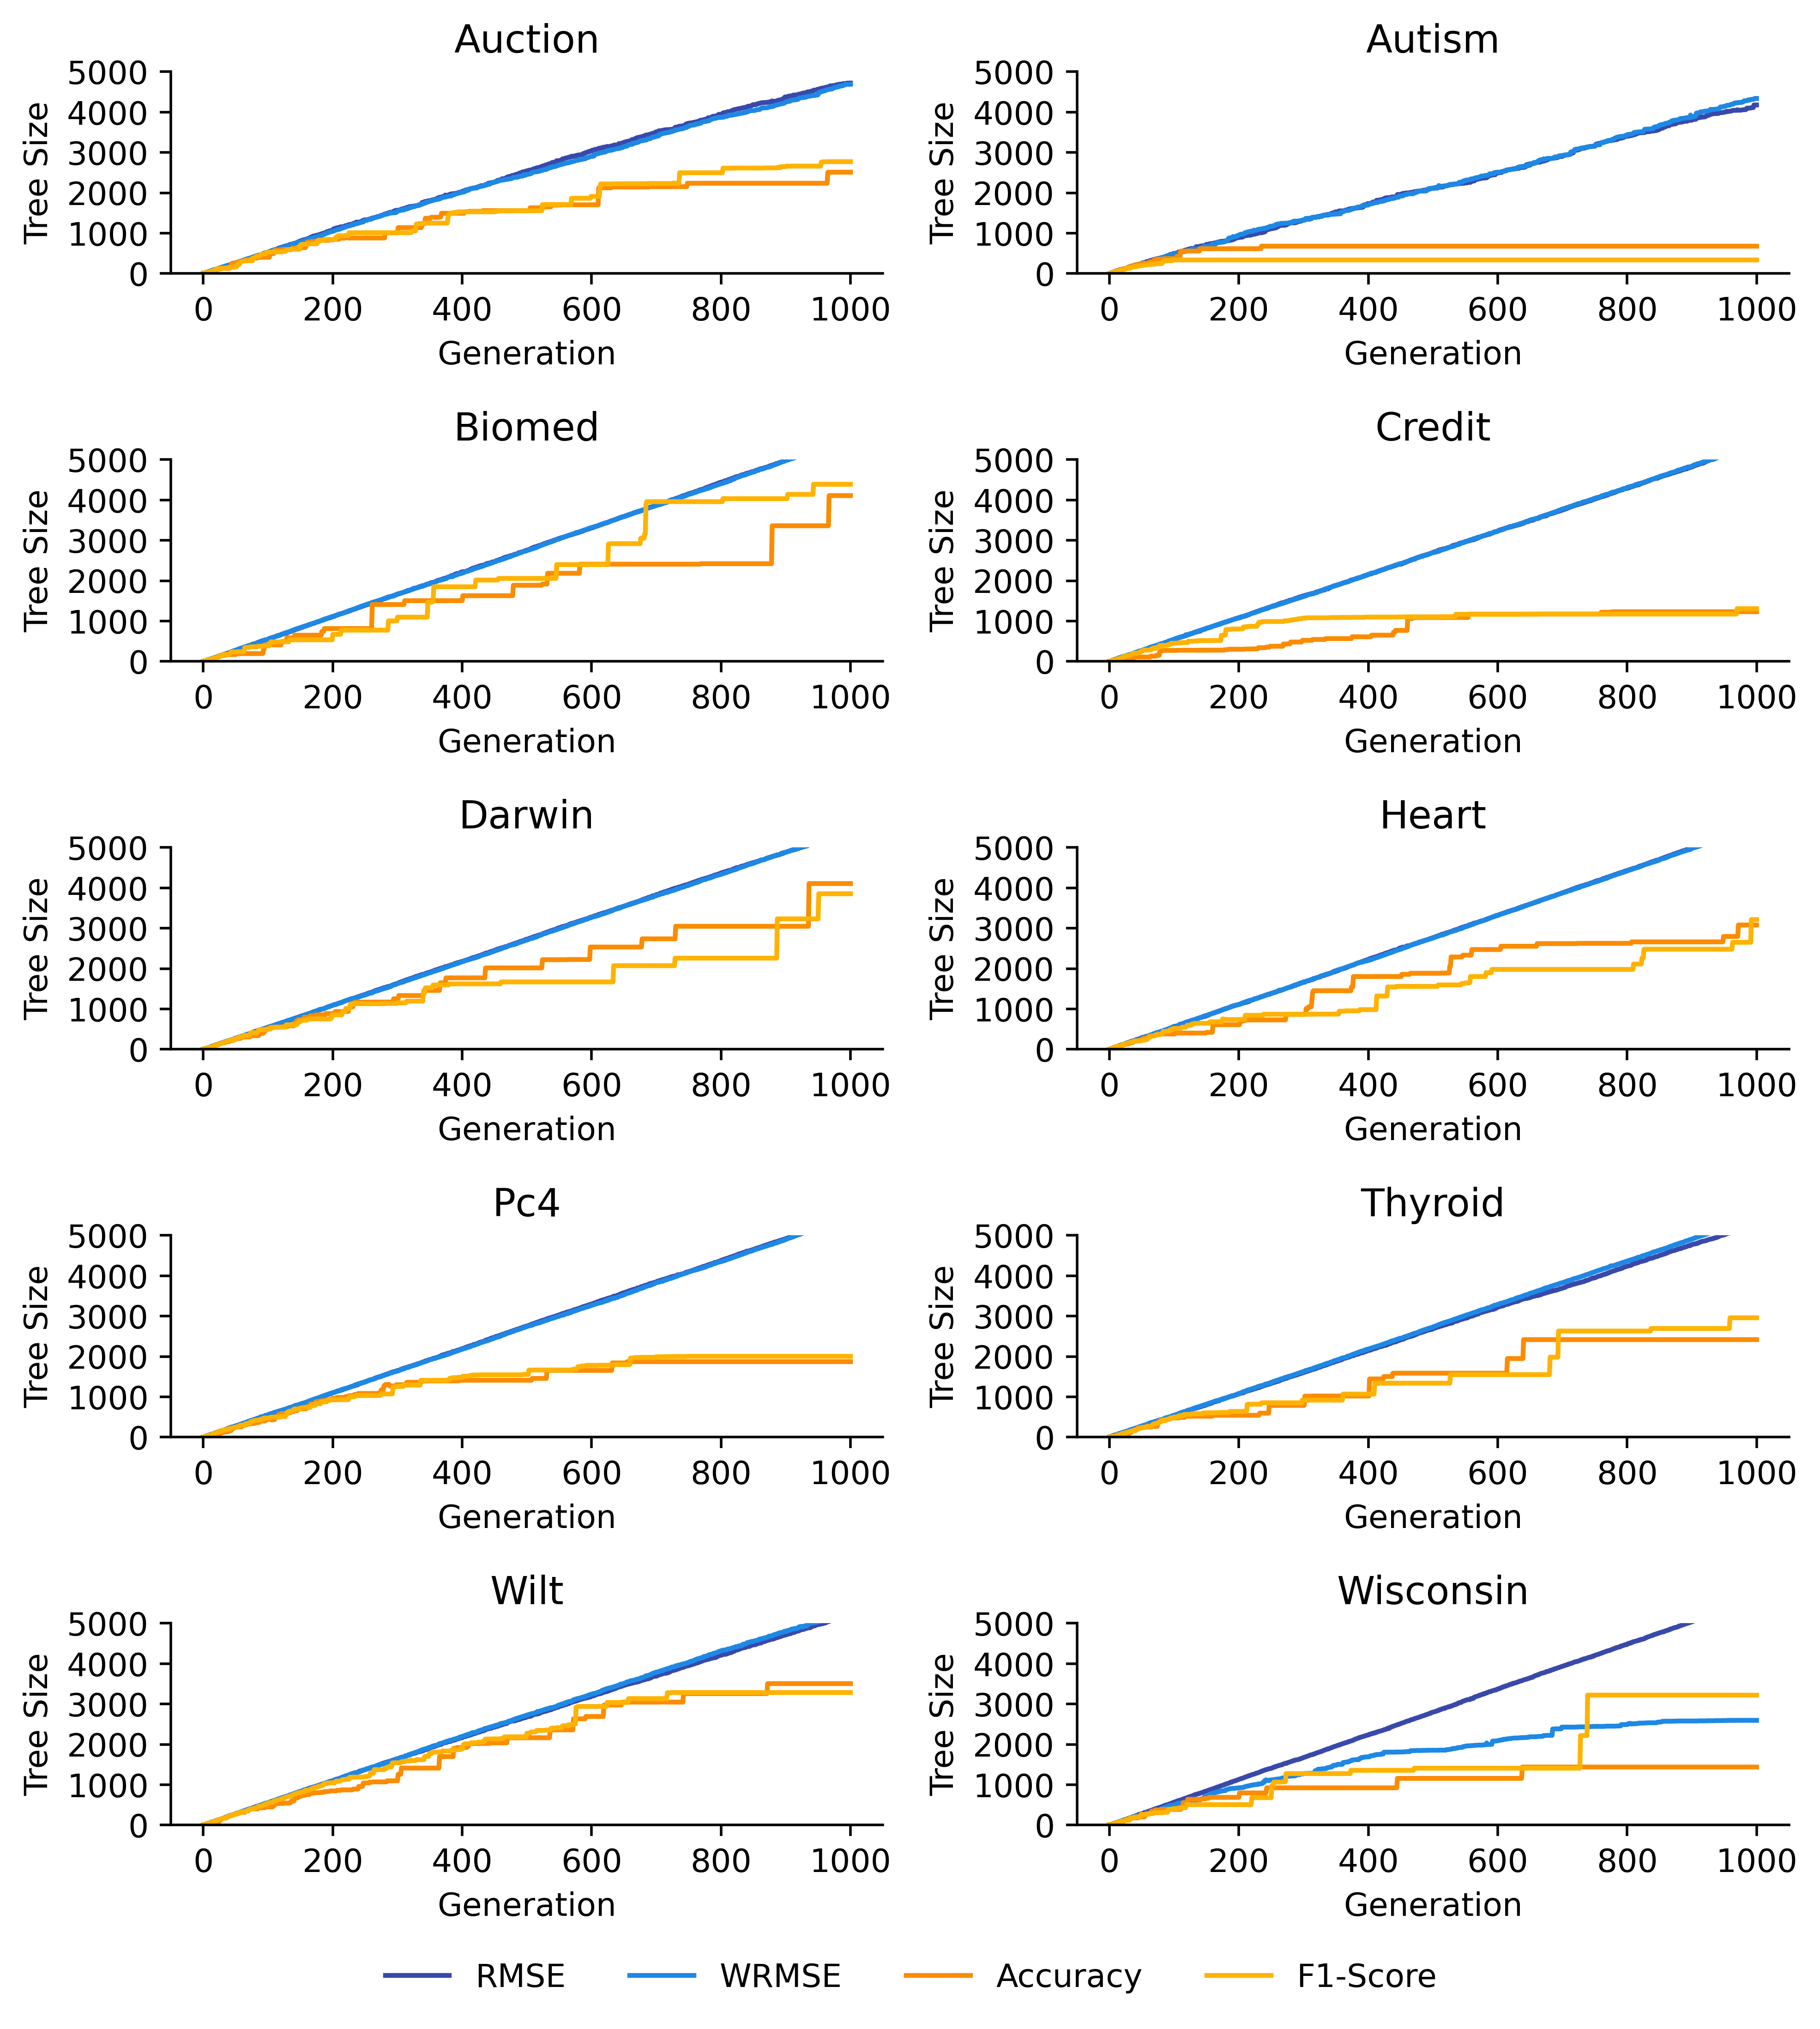
\includegraphics[width=\linewidth]{../Latex/Chapters/Figures/Results/fitness_tree_size_evolution.png}
    \caption{Tree Size Evolution by Fitness Function}
    \label{fig:tree_size_evolution}
    \end{figure}
    
We can see an interesting difference regarding the evolution of the tree size between the 
classification based fitness functions and the regression based fitness functions.
The regression based fitness functions RMSE and WRMSE show a continuous evolution of the tree size across generations.
This means that for the regression based fitness functions, at
nearly each generation a new best solution is found.
The same can be said for the classification based fitness functions accuracy and F1-Score, 
but only for the first 100-200 generations. After that, the tree size of the classification based 
fitness functions shows a more stepwise growth,
meaning a new best solution is only found at certain generations.\\
To explain this behaviour, we additionally need to inspect the evolution of the 
fitness function values in figure \ref{fig:RQ_Fitness_performance_evolution}.
This plot shows the median train and test fitness function value of the elite individual at a given generation.
For visualization consistency, we plot RMSE and WRMSE as $1 - \text{RMSE}$ and $1 - \text{WRMSE}$, so that higher is better,
as it is the case for the classification based fitness functions.
We can see that the classification based fitness functions improve rather quickly in the first 100-200 generations,
but then the improvements become smaller and rarer, more stepwise, leading to a stagnation of the fitness function value.\\
This behaviour can be explained by the fact, that that
improvements of the fitness function when combined with the HSF
can only be achieved, if the model output changes from
0 to 1 or from 1 to 0 for at
least one sample.
Within the semantic space before applying the HSF this refers
to
a change of the model output from <0 to >=0
or vice versa. If we consider that the solution space after applying the HSF is equal to $2^{N}$,
where $N$ is the number of samples in the dataset, it becomes less and less likely to find a 
solution that changes the model output for at least one sample and actually leads to an improvement of the fitness function,
the better the elite already is.\\
RMSE and WRMSE in contrast are based on the distances
between the target value and the model output,
after applying the logistic function. Therefore improvements of the 
fitness function can be achieved by minimizing the distances by
just a small amount at each generation. 
If we think of the solution space after applying the logistic function, it remains continuous,
therefore there is always an infinite number of solutions that are better than the current best solution,
except the case that the current best solution is already the optimal solution.
This means that the distance based fitness functions give smoother
and more detailed feedback at each generation,
whereas in contrast the classification based fitness functions offer only
rough, discrete feedback, which make the search slower
and more likely to get stuck with increasing number of generations. This is part of
the reason why the distance based fitness functions seem to
perform better in terms
of prediction quality as we will show later in the next paragraphs. A downside associated with this behaviour
is that the small improvements
also lead to individuals  of larger size, when compared to the accuracy and F1-Score based fitness functions.\\
The comparison of the achieved median performances considering the evaluation
metrics accuracy, F1-Score and ROC-AUC can be found in
Figure \ref{fig:RQ_Fitness_performance}. %
    \begin{figure}[H]
    \centering
    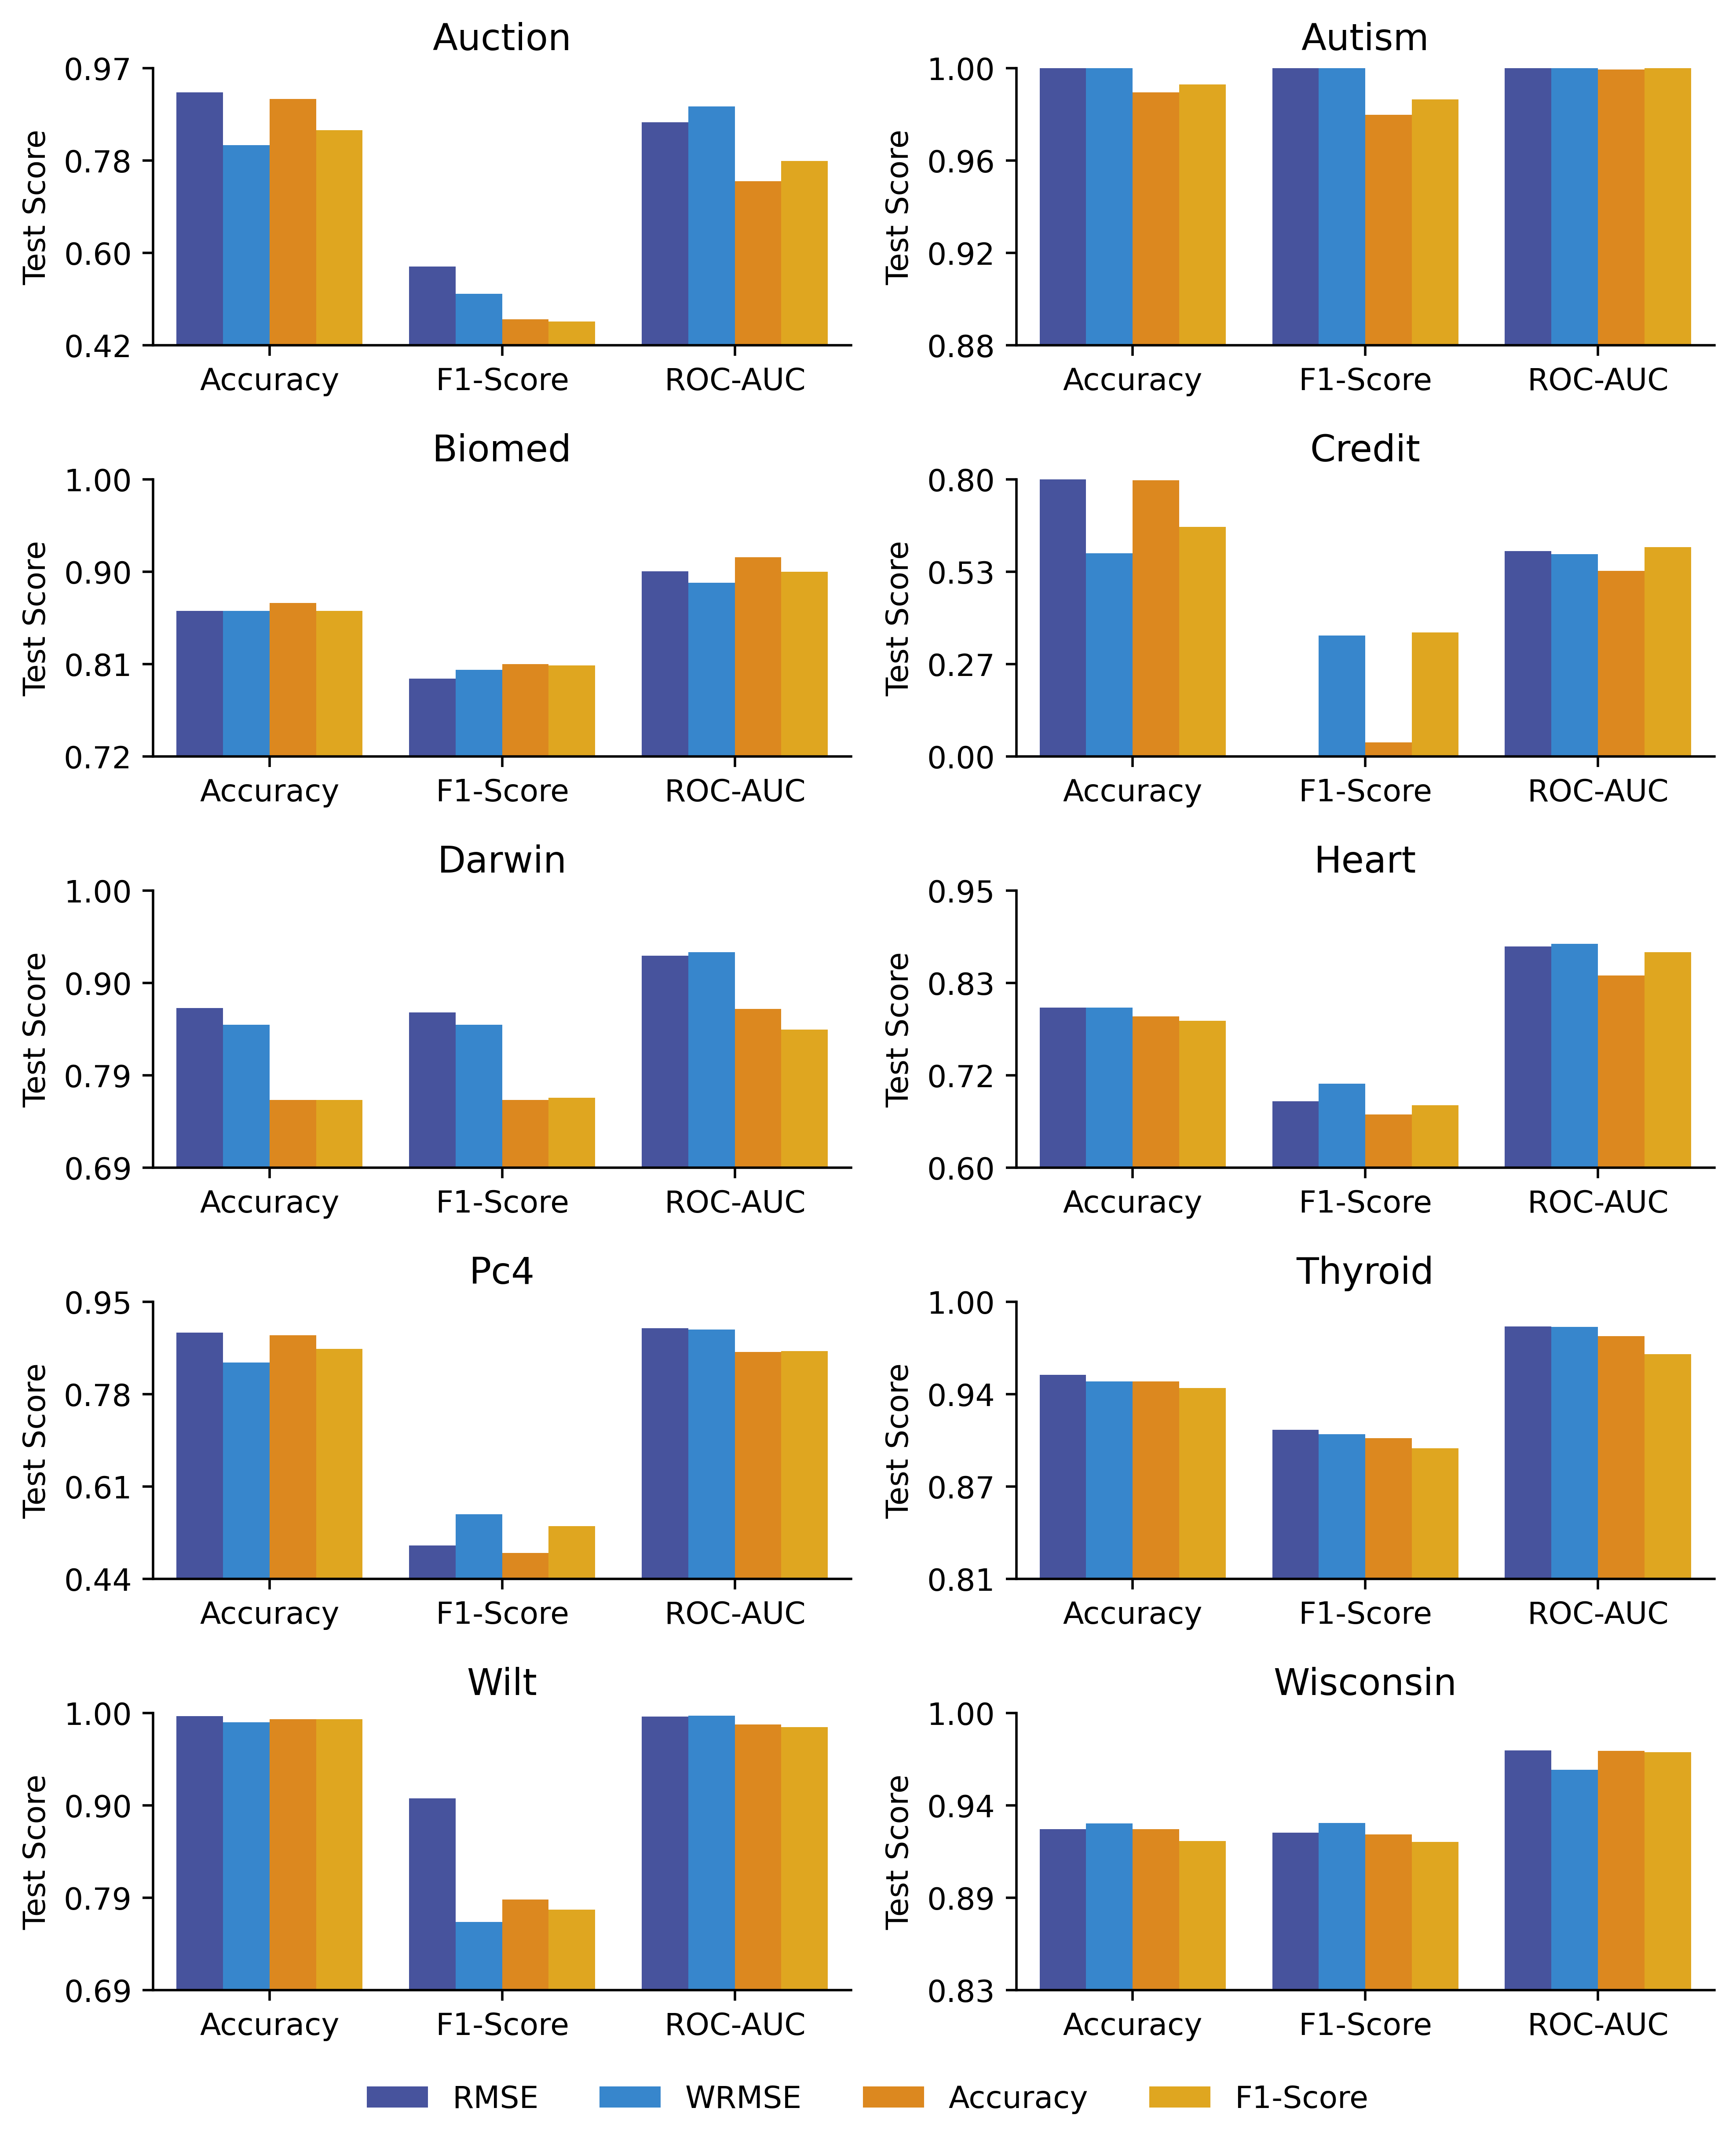
\includegraphics[width=\linewidth]{../Latex/Chapters/Figures/Results/fitness_performance.png}
    \caption{Performance by Fitness Function}
    \label{fig:fitness_performance}
    \end{figure}
    
For each dataset and evaluation metric we performed a pairwise
Wilcoxon rank sum test to determine weather the performances
of two different fitness functions differ significantly at a 5\%
level.
Based on the p-values we created a win-tie-loss table, which
can be found in Table \ref{tab:RQ_Fitness_wtl}.

    \begin{table}[H]
        \centering
        \renewcommand{\arraystretch}{1.2}
        \caption{Win Tie Loss}
        \label{tab:RQ_Fitness_wtl}
    \begin{tabular}{lcccc}
\toprule
Fitness Function & Accuracy & F1-Score & ROC-AUC & Tree Size \\
\midrule
Accuracy vs F1-Score & 3-7-0 & 0-8-2 & 0-8-2 & 0-9-1 \\
Accuracy vs RMSE & 0-4-6 & 1-4-5 & 0-3-7 & 10-0-0 \\
Accuracy vs WRMSE & 4-4-2 & 0-5-5 & 1-2-7 & 10-0-0 \\
F1-Score vs RMSE & 0-4-6 & 1-5-4 & 0-5-5 & 10-0-0 \\
F1-Score vs WRMSE & 4-3-3 & 0-5-5 & 1-2-7 & 10-0-0 \\
RMSE vs WRMSE & 4-6-0 & 2-5-3 & 0-9-1 & 0-10-0 \\
\bottomrule
\end{tabular}

        
    \end{table}
    
\noindent A win/loss means that the performance of the first fitness
function is significantly better/worse than the performance of the second
fitness function.
A tie means that the performance of both fitness functions are not significantly different.\\
We can see that using the accuracy as the fitness
function tends to lead to a better accuracy
than using the WRMSE or the F1-Score as the fitness
function, which is expected since optimizing for
the F1-Score or WRMSE on datasets with a higher degree
of class imbalance, typically goes along with trading off accuracy.
When compared to using the RMSE as the fitness function, the accuracy performs worse on 7 datasets.\\
In terms of F1-Score the WRMSE performs better than the using the F1-Score as the fitness function on 5 datasets.
Interestingly, also the unweighted RMSE performs better than the F1-Score on 4 datasets in terms of F1-Score,
and only gets outperformed once. Also the RMSE performs better than the WRMSE on 2 datasets in terms of F1-Score,
which is surprising, since the WRMSE is designed to address the class imbalance problem. The two datasets where 
RMSE outperforms WRMSE in terms of F1-Score are Auction and Wilt, which both have a high degree of class imbalance.
Therefore a possible explanation could be that WRMSE tends to overpredict the minority class in these cases, leading to a
high recall but low precision, which is penalized by the F1-Score. In terms of ROC-AUC
both regression based fitness functions outperform the classification based fitness functions on at least half of the datasets.

    \begin{figure}[H]
    \centering
    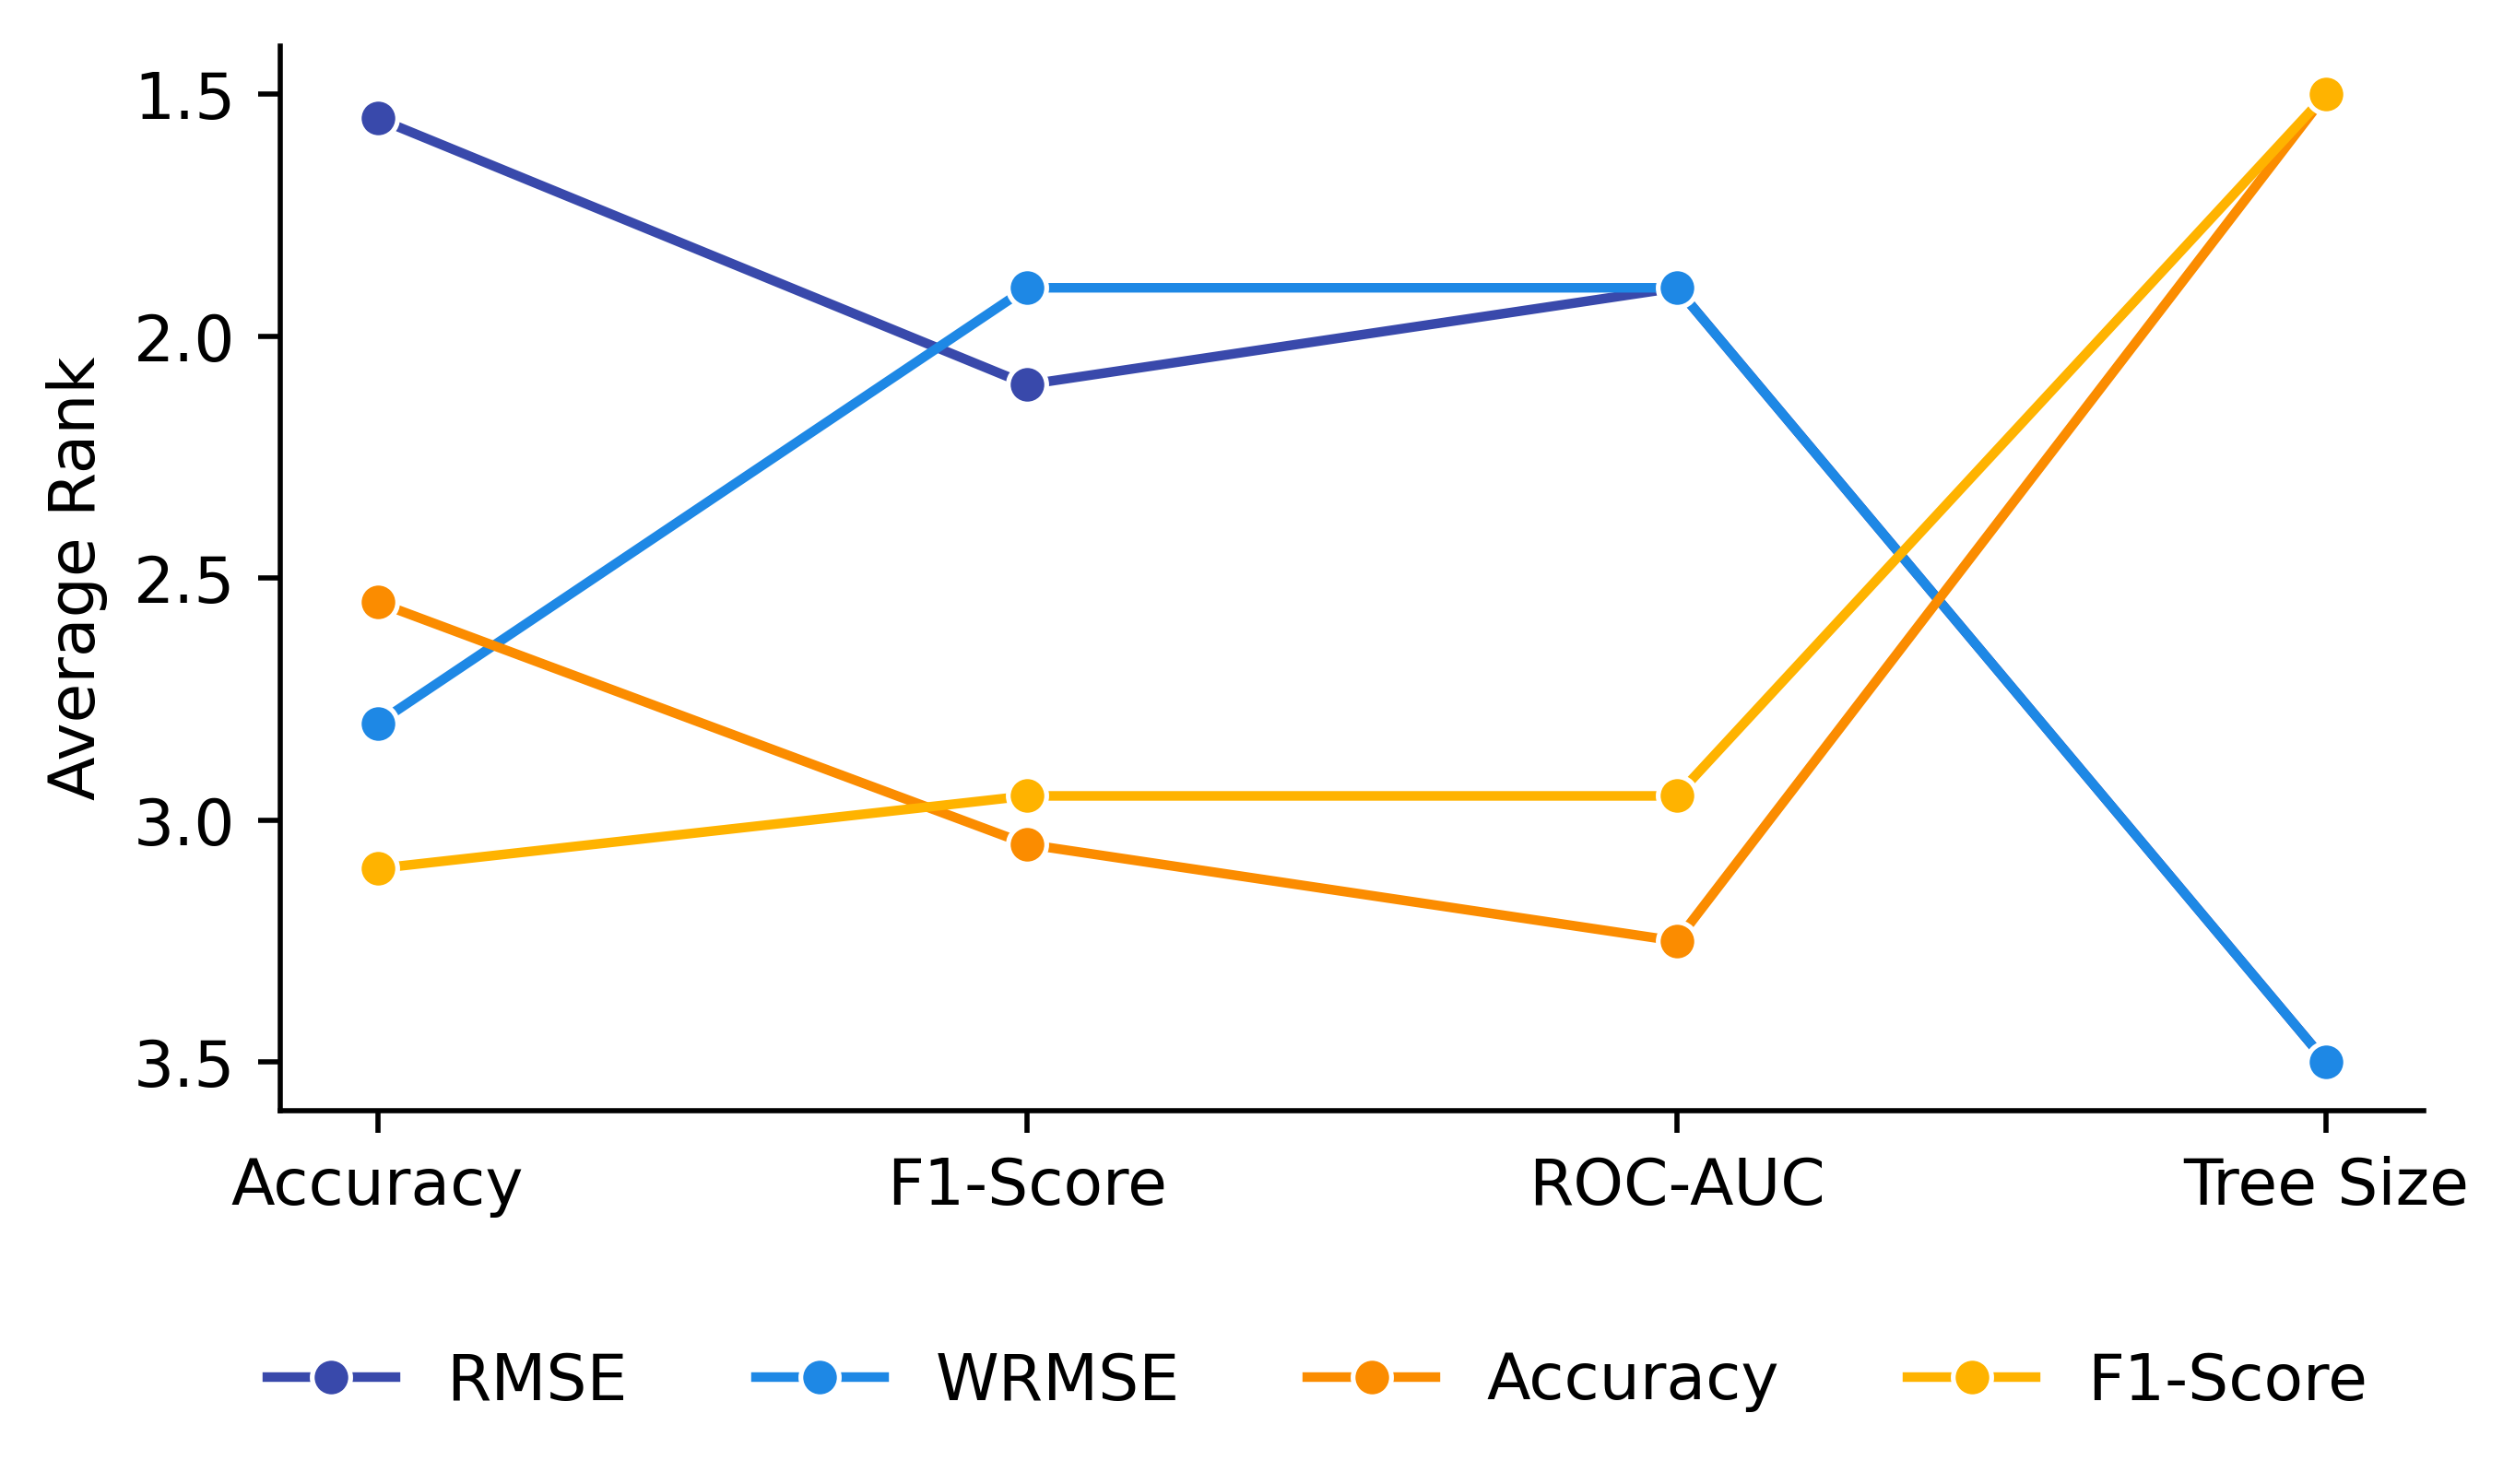
\includegraphics[width=\linewidth]{../Latex/Chapters/Figures/Results/RQ_Fitness_ranks.png}
    \caption{Ranks by Fitness Function}
    \label{fig:RQ_Fitness_ranks}
    \end{figure}
    
\noindent Figure \ref{fig:RQ_Fitness_ranks} shows the mean ranks of the fitness functions
across datasets based on the win-tie-loss table.
For each dataset the ranks of the fitness functions are
calculated as $Rank = 1 + 0.5 \cdot N_{Ties} +
1 \cdot N_{Losses}$.
As a consequence a rank of 1 means that the
fitness function outperformed all other fitness functions,
whereas a rank of 4 means that the fitness function
was outperformed by all other fitness functions.
This figure essentially summarizes the superior performance of the regression-based fitness functions.\\
Table \ref{tab:RQ_Fitness_friedman} shows the results of the Friedman test, that
was performed to determine if there are any
significant differences at a 5\% level between the fitness functions. As we can see the ranks for all evaluation metrics are significant.

    \begin{table}[H]
        \centering
        \renewcommand{\arraystretch}{1.2}
        \caption{p-Values of the Friedman Test}
        \label{tab:RQ_Fitness_friedman}
    \begin{tabular}{lcc}
\toprule
Metric & P-Value & Significant \\
\midrule
Accuracy & 0.006961 & Yes \\
F1-Score & 0.007536 & Yes \\
ROC-AUC & 0.004693 & Yes \\
Tree Size & 0.000002 & Yes \\
\bottomrule
\end{tabular}

        
    \end{table}
    
\subsubsection{Interpretation}
The results of Experiment 1 reveal clear differences between classification-based and regression-based fitness functions, 
both in terms of optimization behavior and prediction quality.
Regression-based functions (RMSE, WRMSE) lead to a smoother search process, 
with continuous improvements across generations. This is because the search space remains continuous after applying the logistic function,
therefore even small output changes can improve the fitness.
In contrast, classification-based functions (accuracy, F1-Score) rely on discrete output shifts after applying the HSF, 
whereas further improvements become rarer as the individuals improve, which explains the stepwise tree growth and more frequent stagnation.\\
Performance-wise, accuracy as a fitness function naturally leads to better accuracy than WRMSE or F1-Score,
but gets outperformed by RMSE and struggles on F1-Score and ROC-AUC, 
particularly with imbalanced datasets. 
Both regression-based functions (RMSE, WRMSE) outperform classification-based functions on F1-Score and ROC-AUC in most of the cases.
WRMSE is particularly effective for F1-Score, but RMSE can outperform it on some imbalanced datasets, most likely due to the tendency
of WRMSE to overpredict the minority class, leading to high recall but low precision.\\
In conclusion, our analysis of fitness function impact reveals that 
the choice of fitness function significantly affects both prediction quality and tree size. 
Regression-based functions, are more effective for guiding the search of the GSGP algorithm leading to better performance, 
while classification-based functions may be preferable when simplicity is prioritized.

\subsection{Experiment 2: The impact of the inflation rate}
\label{sec:exp2}
\subsubsection{Experimental Settings}
The configurations used to evaluate the impact of the inflation rate 
are listed in Table~\ref{tab:hyperparametersslim}. 
We chose to apply two versions of the SLIM-GSGP algorithm: SLIM+SIG1 and SLIM*SIG1. 
This allows us to include both an addition-based and a multiplication-based variant. 
We specifically selected the versions that use only a single random function, as 
our goal is to optimize not only for predictive performance but also for model simplicity. 
We chose the SIG1 expression over the ABS variant because we consider the use of
absolute values to be less intuitively interpretable than the application of a logistic function.\\
The inflation rate is set to 0.1, 0.3, 0.5 and
0.9,
which means that the deflation mutation operator is applied with
a probability of 0.9, 0.7, 0.5 and 0.1 respectively. The higher the inflation rate, the 
more similar the SLIM-GSGP algorithm behaves to traditional GSGP, since SLIM+SIG2 with an inflation rate of 1.0
is equivalent to GSGP with a mutation probability of 1.0 and crossover probability of 0.0.
Therefore, to capture the whole landscape, we additionally included the inflation rate of 0.9, 
to the more typical values \cite{Vanneschi2024} of 0.1, 0.3 and 0.5.
Furthermore, like in the first experiment, choose different upper bounds
of the uniform distribution, of which the mutation step is
selected from at each inflate mutation, including the more typical values \cite{Vanneschi2024} of 0.1, 0.5 and 1.0 and the larger value of 5.0.
The combination of the inflation rate and mutation upper step is applied for both versions of the SLIM-GSGP algorithm,
leading
to a total of 32 different grid search configurations.\\
The fitness function used for this experiment is the RMSE
in combination with the logistic function, 
as it matches the original introduction of GSGP for binary classification by \cite{Bakurov2019} 
and led to results among the best in the first experiment.
\input{Tables/Setup/hyperparametersslim.tex}
\subsubsection{Results}
We start by analyzing the impact of the inflation rate
and the upper bound of the mutation step on the
tree size. Figure \ref{fig:RQ_Inflationrate_tree_size_by_p_inflate}
shows the median tree size for the different inflation rates and mutation upper steps.\\
%
    \begin{figure}[h]
    \centering
    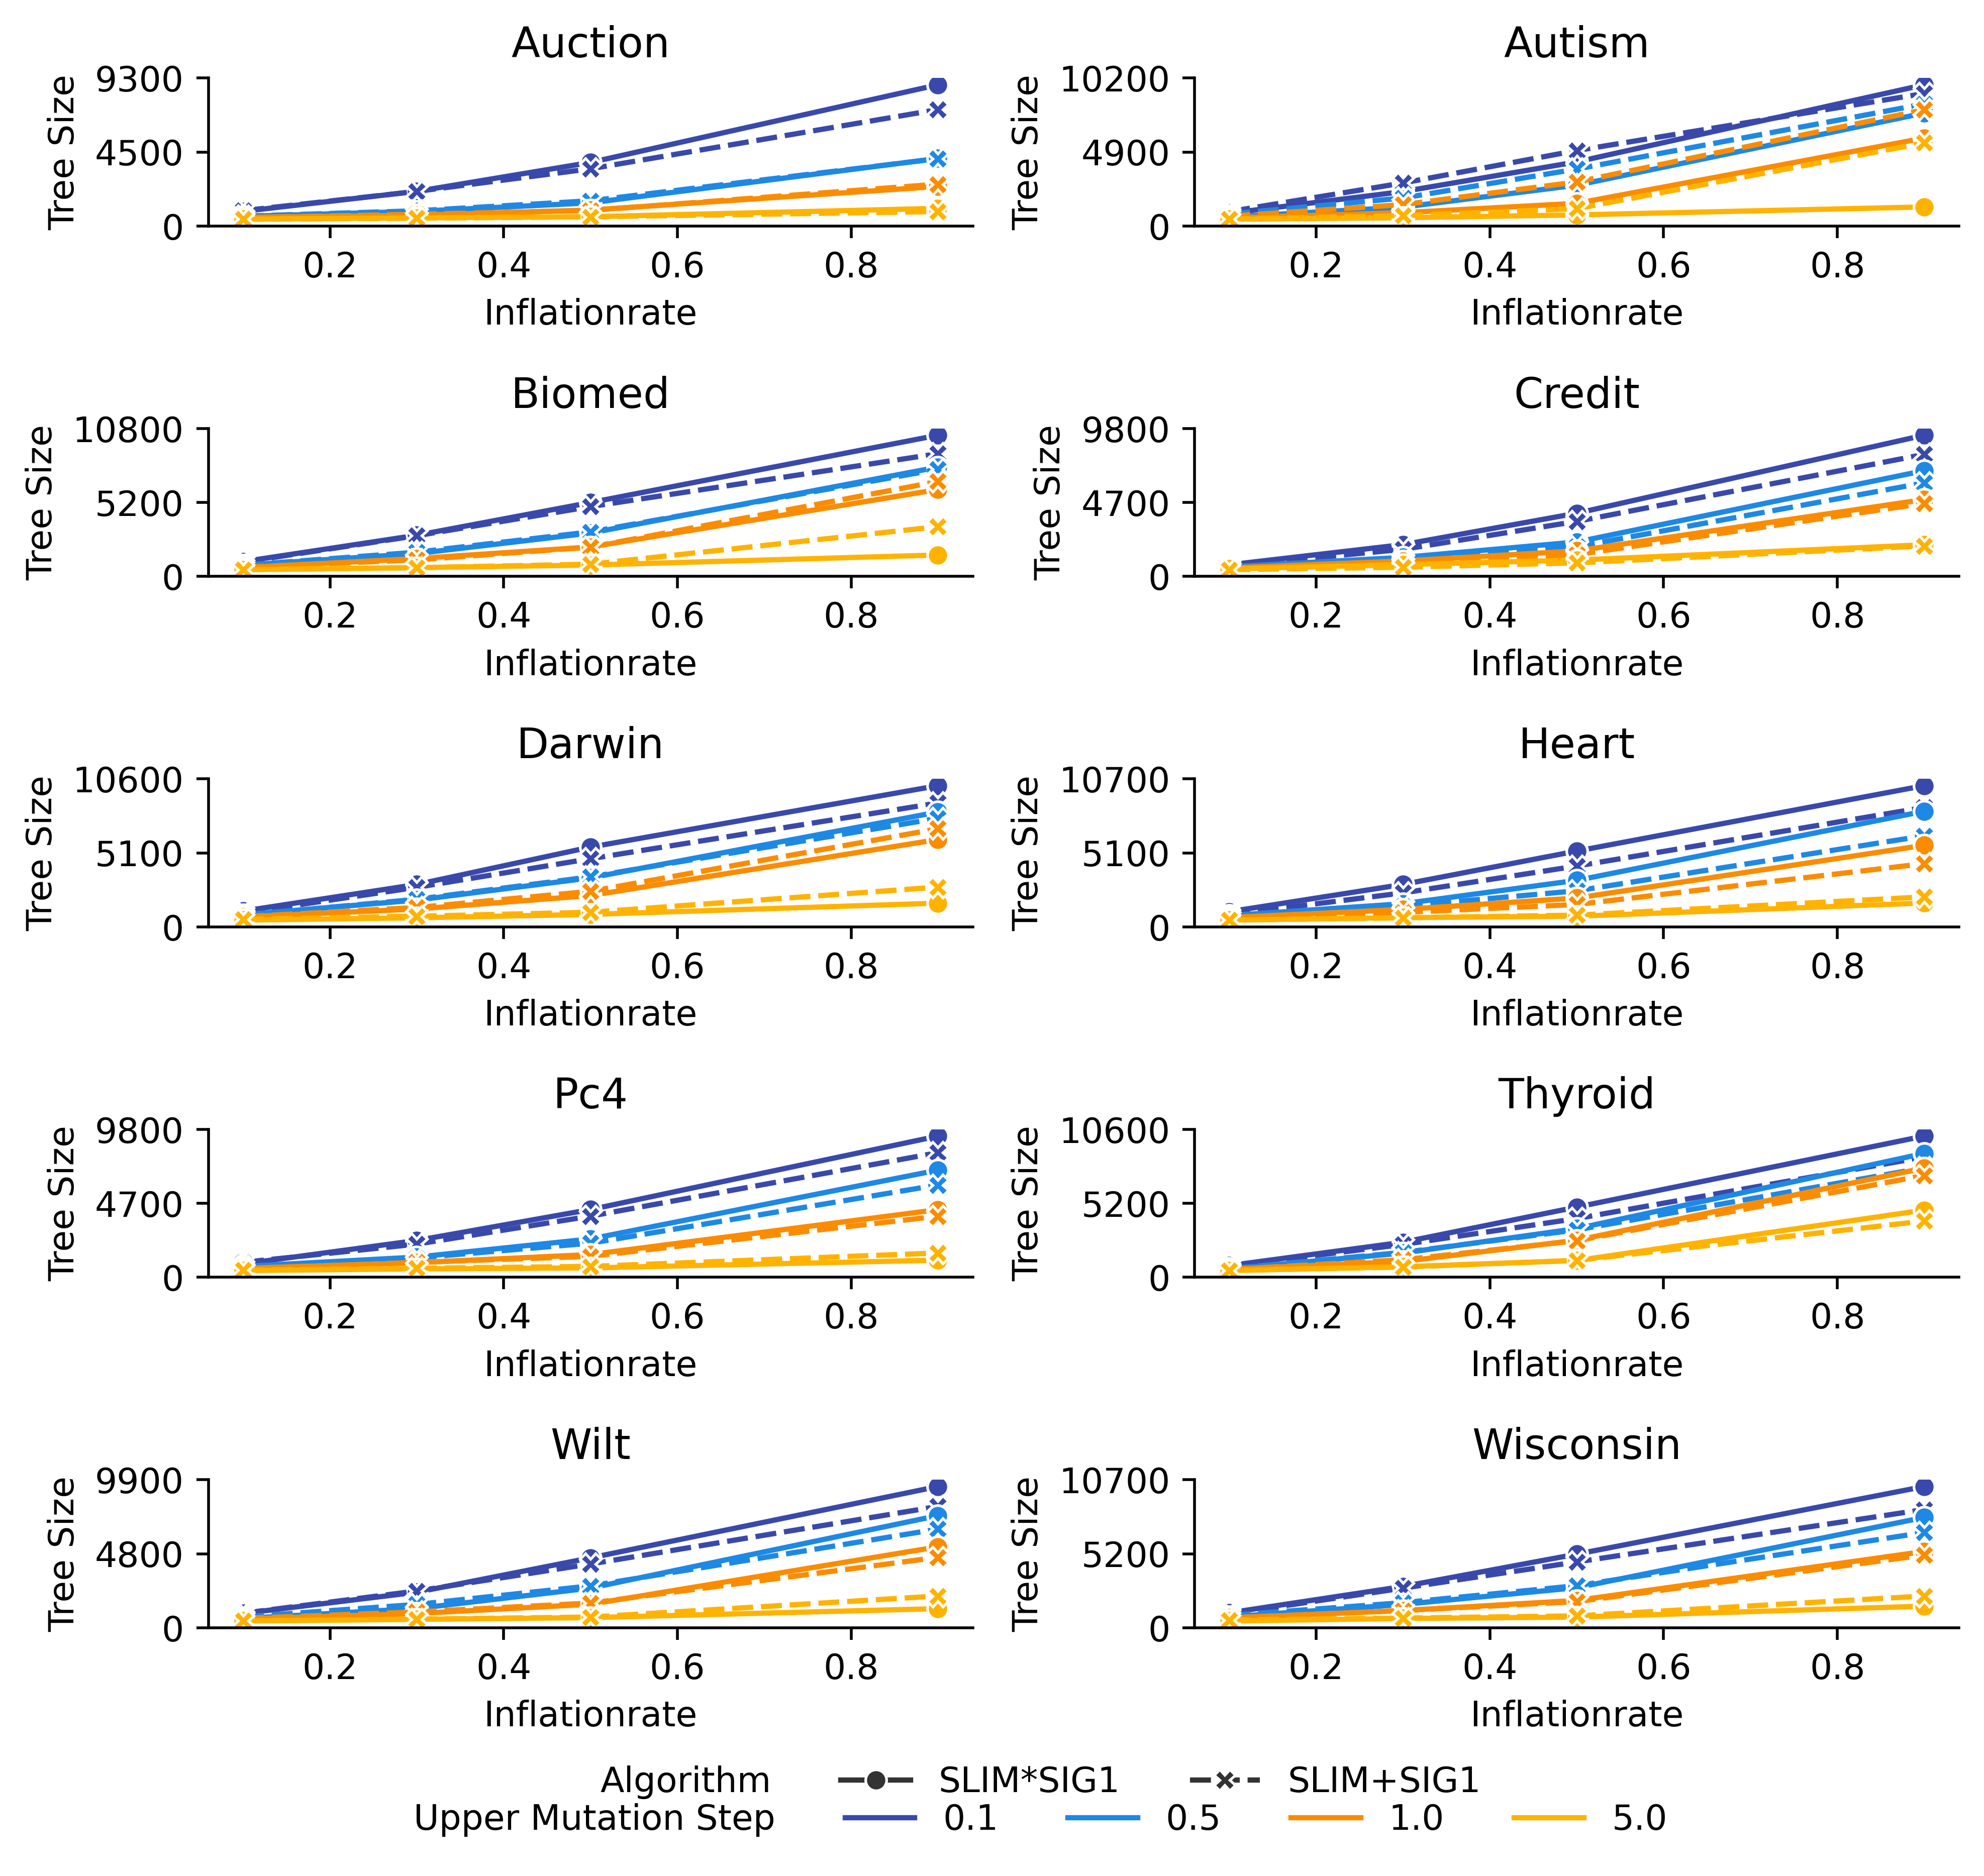
\includegraphics[width=\linewidth]{../Latex/Chapters/Figures/Results/inflationrate_tree_size_by_p_inflate.png}
    \caption{Tree Size by Inflationrate}
    \label{fig:tree_size_by_p_inflate}
    \end{figure}
    
The trend of the impact of the inflation rate on
the tree size is similar for both versions of SLIM-GSGP:
The higher the inflation rate, the larger the individuals. This
of course is expected, since
the higher the inflation rate, the higher the probability of
applying the inflation mutation operator, which leads to larger individuals.
The mutation upper step bound has the opposite effect: The
higher the mutation upper step, the smaller the individuals.
Also this is expected, since the higher the mutation upper step, the larger the possible movement of the individuals
in the semantic space.
Therefore less steps are needed to reach the same semantic distance.\\
Figure \ref{fig:RQ_Inflationrate_performance_by_p_inflate} shows the median RMSE on the train and
test sets for the different inflation rates and mutation upper steps.
In all the cases the RMSE on the training set
decreases with increasing inflation rate, which is expected since the
higher the inflation rate, the more information is
added to the individuals. However, the RMSE on the test
set does not show a clear trend. On some datasets
like Biomed and Credit,
having a lower inflation rate leads to a better performance,
while on others like Auction and Autism the opposite is
the case. For Heart and Pc4
the lowest RMSE is achieved with a low, but not the lowest, inflation rate of 0.3.\\
%
    \begin{figure}[h]
    \centering
    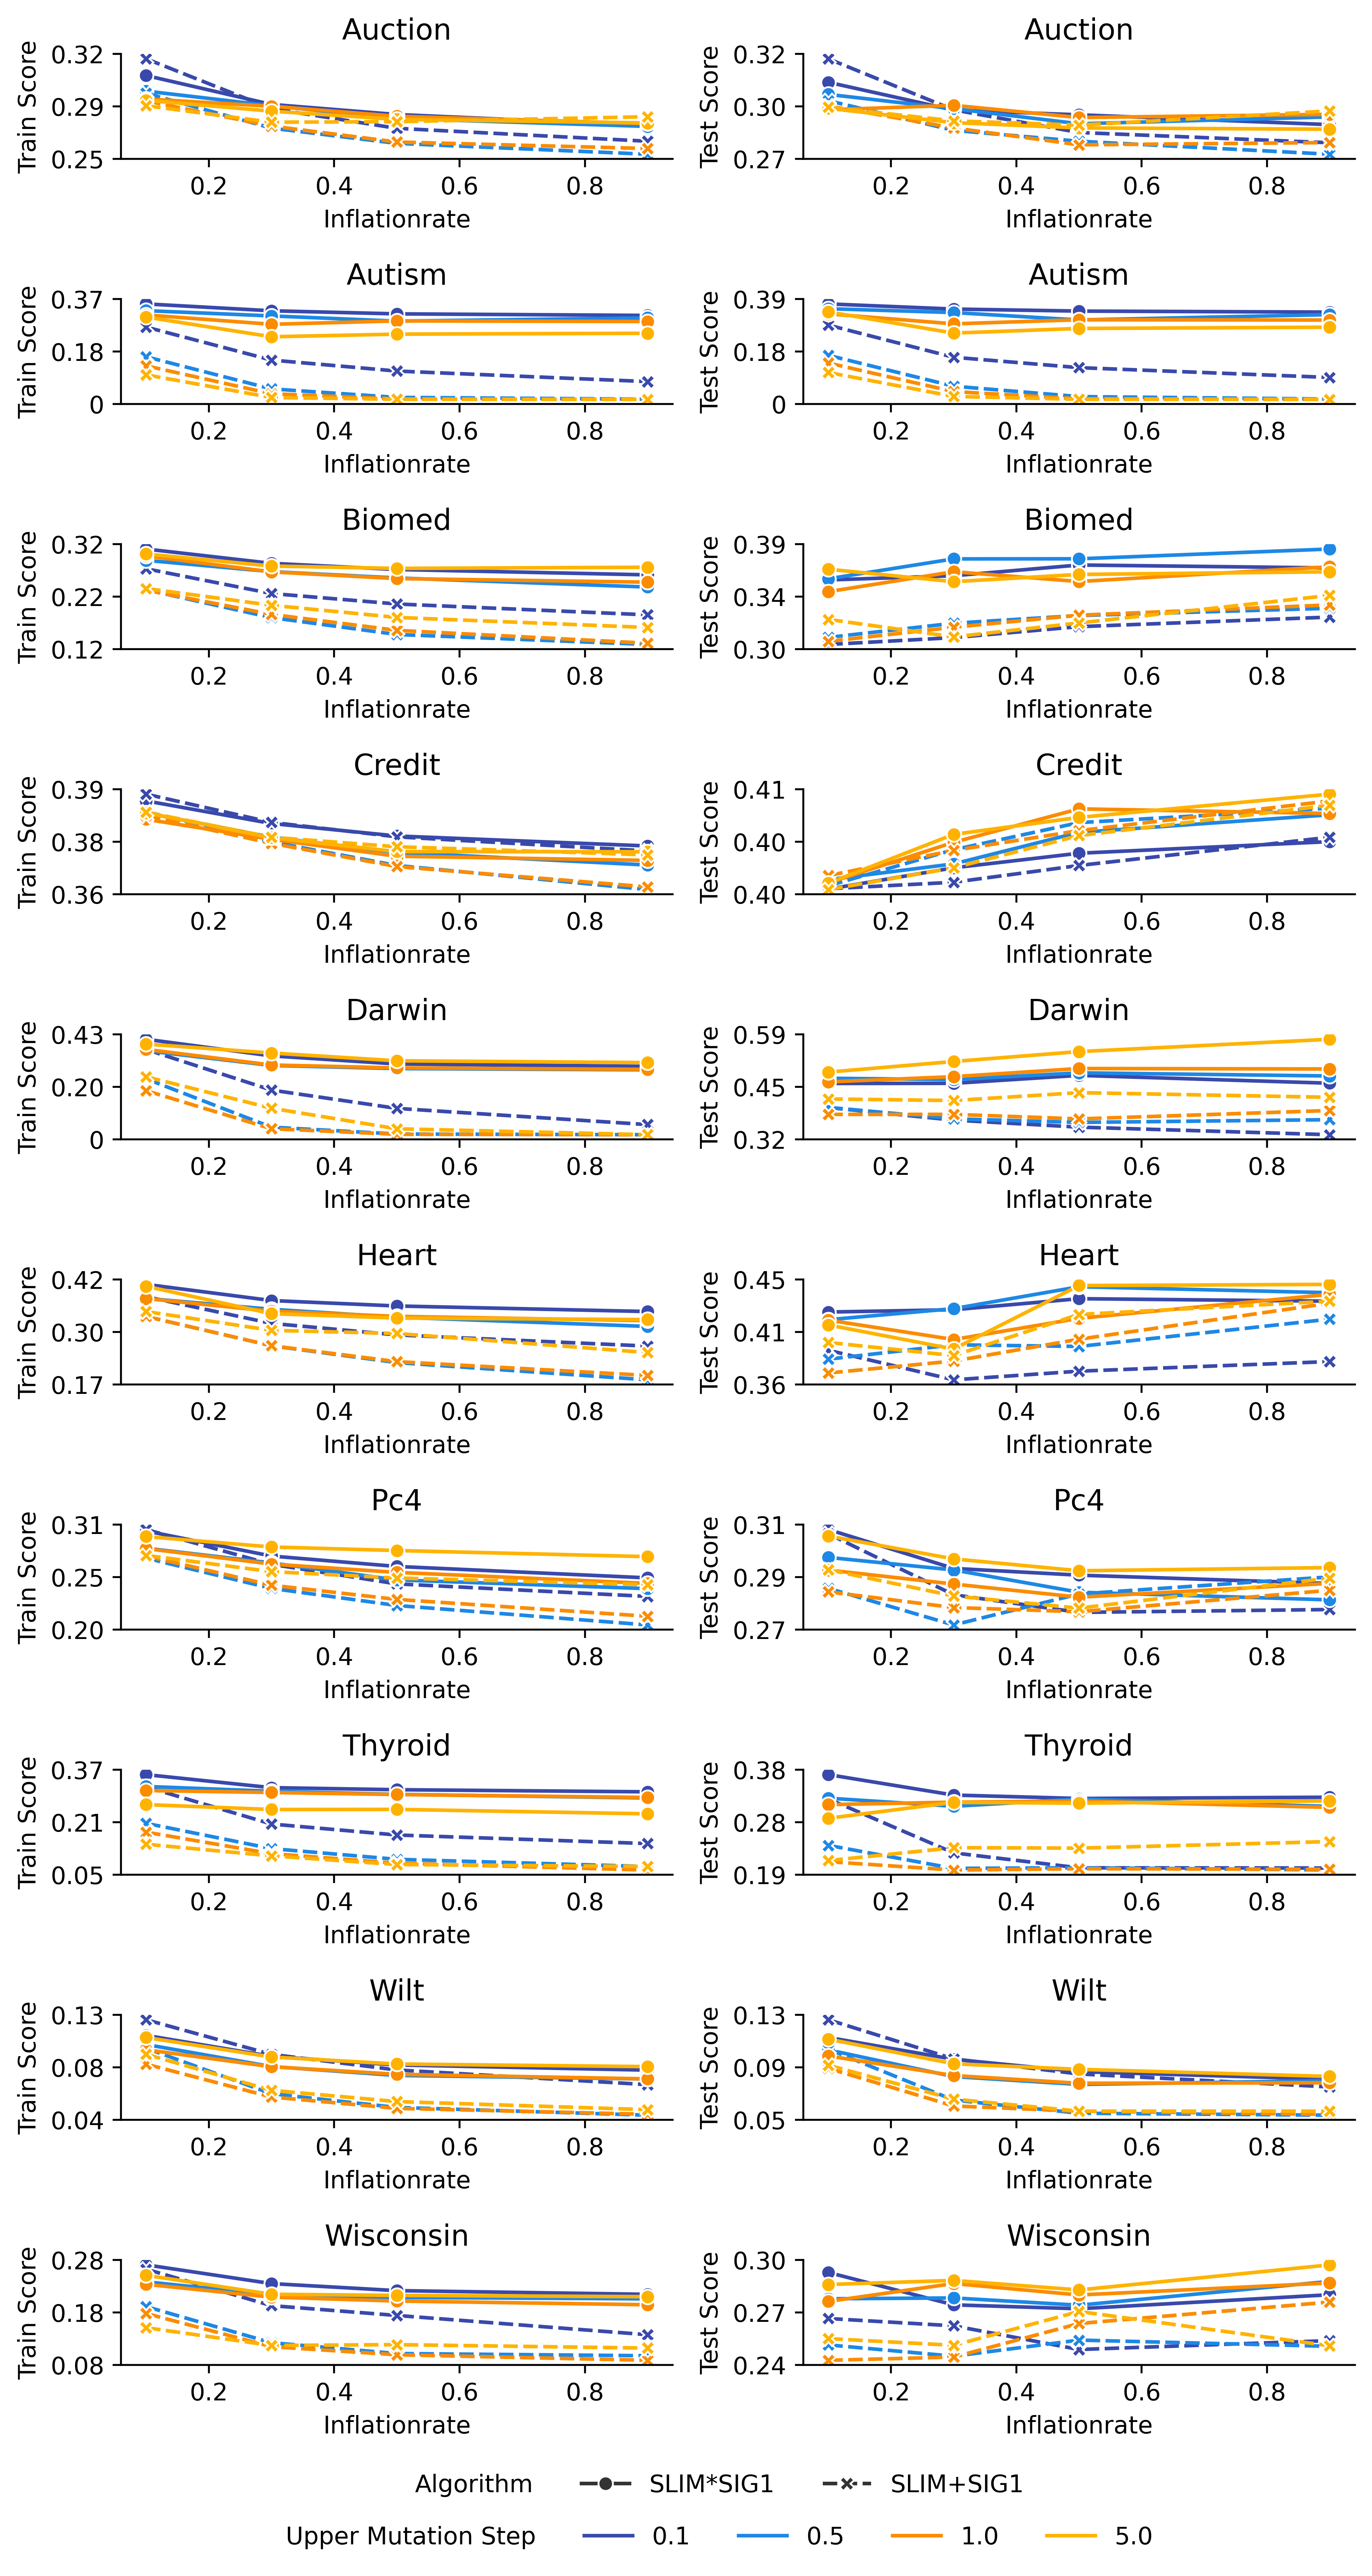
\includegraphics[width=\linewidth]{../Latex/Chapters/Figures/Results/inflationrate_performance_by_p_inflate.png}
    \caption{Performance by Inflationrate}
    \label{fig:performance_by_p_inflate}
    \end{figure}
    
Figures~\ref{fig:RQ_Inflationrate_performance_complexity_tradeoff_mulsig1} 
and~\ref{fig:RQ_Inflationrate_performance_complexity_tradeoff_plussig1} 
show the median RMSE on the test set along the y-axis 
and the median tree size along the x-axis, 
across different settings of inflation rate and mutation upper step. 
These plots help visualize the trade-off between performance and complexity of the individuals.
The mutation upper step is encoded using color, 
while the inflation rate is represented by the size of the markers. 
When comparing individuals of the same color (same mutation upper step) it 
becomes apparent that larger markers (higher inflation rate) 
consistently lead to larger tree sizes. This reflects a positive correlation between inflation rate and model complexity.
The effect of inflation rate on test RMSE, however, 
varies across datasets. In many cases, increasing the inflation rate 
(while keeping the mutation upper step constant) either improves or degrades performance. 
In some datasets, the lowest test RMSE is achieved at an intermediate inflation rate, for example 
in the Pc4 dataset.
Overall, individuals with low test RMSE 
values can be found across a wide range of tree sizes, and no consistent trend emerges across all datasets.\\
Visually speaking, an optimal solution that captures the trade-off between performance and complexity the best
would be found at the bottom left corner of the
plot, meaning the lowest RMSE and a smallest tree size.
In fact,
for both the slim versions and all the datasets, except
the Auction and the Darwin dataset and SLIM+SIG1,
we can find at least one individual, that could be
described as close to the optimal solution.
We want to compare the best individuals just considering the
RMSE on the test set, with an individual that focuses
on the
trade off between performance and complexity. The method used to
decide on a best individual that captures the trade
off between performance and complexity is inspired by Kamal et al. \cite{Kamal2018}, who
used the Euclidian distance to decide on a best compromise
solution
for a multiobjective optimization problem.
We start by normalizing the RMSE and tree size to
a range between 0 and 1 for all configurations, meaning
the different
combinations of inflation rate and mutation step upper bound.
Then we calculate the weighted Euclidean distance of the individuals
to the origin (0,0), which is defined as:
\[
D = \sqrt{w_1 \cdot x_1^2 + w_2 \cdot x_2^2}\]
where $x_1$ and $x_2$ are the normalized RMSE and tree
size respectively and $w_1$ and $w_2$ are the weights of
the two metrics.
Notice that the origin (0,0) relates to the normalized RMSE and tree size
and therefore the origin represents the best solution based on the existing solutions, 
not the theoretically absolute best solution with a RMSE of 0 and a tree size of 0.
We evaluated three different combinations of weights ($w_1$, $w_2$):
\begin{itemize}
    \item $w_1 = 1, w_2 = 1$: This means that we consider the
    RMSE and the tree size as equally important.
    \item $w_1 = 1, w_2 = 2$: This means that we consider the
    tree size as twice as important as the RMSE.
    \item $w_1 = 2, w_2 = 1$: This means that we consider the
    RMSE as twice as important as the tree size.
\end{itemize}
The results remain the same for most of the datasets and version of SLIM-GSGP, no matter which weights we choose.
We decided to do the analysis with the weights ($w_1$, $w_2$) set to (1,2),
since we believe it captures the trade off the best.
For each dataset we choose the individual with the minimal
weighted distance to the origin as the best individual considering
the trade off between
performance and complexity. Notice that following this approach, 
the best individual will always be part of the pareto optimal set.\\

    \begin{table}[H]
        \centering
        \renewcommand{\arraystretch}{1.2}
        \caption{Tradeoff between Performance and Complexity}
        \label{tab:RQ_Inflationrate_tradeoff}
    \begin{tabular}{lccccccccccc}
\toprule
Dataset & Version & \multicolumn{2}{r}{Inflationrate} & \multicolumn{2}{r}{Upper MS} & \multicolumn{2}{r}{RMSE} & RMSE \% & \multicolumn{2}{r}{Tree Size} & Tree Size \% \\
 &  &  R &  T &  R &  T &  R &  T &  &  R &  T &  \\
\midrule
Auction & SLIM*SIG1 & 0.500000 & 0.500000 & 5.000000 & 5.000000 & 0.286600 & 0.286600 & +0.0\% & 232.500000 & 232.500000 & 0.0\% \\
Auction & SLIM+SIG1 & 0.900000 & 0.500000 & 0.500000 & 1.000000 & 0.273000 & 0.281200 & +3.0\% & 4066.500000 & 654.500000 & -83.9\% \\
Autism & SLIM*SIG1 & 0.500000 & 0.500000 & 5.000000 & 5.000000 & 0.214900 & 0.214900 & +0.0\% & 344.000000 & 344.000000 & 0.0\% \\
Autism & SLIM+SIG1 & 0.900000 & 0.300000 & 5.000000 & 5.000000 & 0.000000 & 0.007000 & +inf\% & 5731.500000 & 319.000000 & -94.4\% \\
Biomed & SLIM*SIG1 & 0.100000 & 0.100000 & 1.000000 & 1.000000 & 0.339100 & 0.339100 & +0.0\% & 346.500000 & 346.500000 & 0.0\% \\
Biomed & SLIM+SIG1 & 0.100000 & 0.100000 & 1.000000 & 1.000000 & 0.303600 & 0.303600 & +0.0\% & 327.000000 & 327.000000 & 0.0\% \\
Credit & SLIM*SIG1 & 0.100000 & 0.100000 & 5.000000 & 5.000000 & 0.396000 & 0.396000 & +0.0\% & 158.500000 & 158.500000 & 0.0\% \\
Credit & SLIM+SIG1 & 0.100000 & 0.100000 & 5.000000 & 5.000000 & 0.396900 & 0.396900 & +0.0\% & 114.500000 & 114.500000 & 0.0\% \\
Darwin & SLIM*SIG1 & 0.100000 & 0.100000 & 0.100000 & 0.100000 & 0.445800 & 0.445800 & +0.0\% & 713.500000 & 713.500000 & 0.0\% \\
Darwin & SLIM+SIG1 & 0.900000 & 0.300000 & 0.100000 & 0.500000 & 0.319500 & 0.348100 & +9.0\% & 8771.000000 & 1587.000000 & -81.9\% \\
Heart & SLIM*SIG1 & 0.100000 & 0.100000 & 5.000000 & 5.000000 & 0.411600 & 0.411600 & +0.0\% & 102.500000 & 102.500000 & 0.0\% \\
Heart & SLIM+SIG1 & 0.300000 & 0.100000 & 0.100000 & 0.500000 & 0.380700 & 0.382000 & +0.3\% & 2255.000000 & 386.500000 & -82.9\% \\
Pc4 & SLIM*SIG1 & 0.500000 & 0.500000 & 0.500000 & 1.000000 & 0.281500 & 0.282500 & +0.4\% & 2080.500000 & 1155.000000 & -44.5\% \\
Pc4 & SLIM+SIG1 & 0.500000 & 0.500000 & 0.100000 & 5.000000 & 0.277200 & 0.278400 & +0.4\% & 3831.000000 & 345.000000 & -91.0\% \\
Thyroid & SLIM*SIG1 & 0.500000 & 0.100000 & 5.000000 & 5.000000 & 0.311100 & 0.312800 & +0.5\% & 982.000000 & 174.000000 & -82.3\% \\
Thyroid & SLIM+SIG1 & 0.900000 & 0.100000 & 0.100000 & 1.000000 & 0.201100 & 0.207800 & +3.4\% & 8634.500000 & 297.500000 & -96.6\% \\
Wilt & SLIM*SIG1 & 0.500000 & 0.300000 & 0.500000 & 1.000000 & 0.080200 & 0.085300 & +6.4\% & 2294.500000 & 629.000000 & -72.6\% \\
Wilt & SLIM+SIG1 & 0.900000 & 0.500000 & 0.500000 & 5.000000 & 0.054500 & 0.058700 & +7.6\% & 6447.500000 & 413.000000 & -93.6\% \\
Wisconsin & SLIM*SIG1 & 0.500000 & 0.100000 & 0.500000 & 5.000000 & 0.265500 & 0.270100 & +1.7\% & 2582.000000 & 122.000000 & -95.3\% \\
Wisconsin & SLIM+SIG1 & 0.100000 & 0.100000 & 0.500000 & 0.500000 & 0.222100 & 0.222100 & +0.0\% & 452.000000 & 452.000000 & 0.0\% \\
\bottomrule
\end{tabular}
\end{table}
    
\noindent Table \ref{tab:RQ_Inflationrate_tradeoff_r1_t2} shows the comparison of the best individual considering
the RMSE on the test set, denoted as R,
and the best individual considering the trade off between performance
and complexity, denoted as T, following the approach described above.
The results for the other weights can be found in the appendix 
\ref{tab:RQ_Inflationrate_tradeoff_r1_t1} and \ref{tab:RQ_Inflationrate_tradeoff_r2_t1}.
As we can see, in some cases the best individual
considering the RMSE on the test set is also the
best individual considering the trade off between performance and complexity.
In other cases,
the RMSE of the best individuals regarding the trade off
is only larger by a small percentage than the RMSE
of the best individual considering the RMSE on the test
set.
On the other hand, the tree size of the best
individual considering the trade off is always smaller, most times by
multiples,
than the tree size of the best individual considering only
the RMSE on the test set.
Therefore we can see that the inflation rate does not only help
to reduce the size of the individuals, but also has
a regularization effect,
that can help to avoid overfitting and therefore improve the
performance on the test set. Even when the best performance
on the test set
is achieved with a high inflation rate, associated with a
large individual, we can find an individual with another combination
of inflation rate and mutation upper step, of way
smaller size that achieves an only slightly worse performance.
\subsubsection{Example of how smaller models increase interpretability}
According to Lipton \cite{Lipton2016} an interpretable model should be transparent, whereas simulatability and decomposability are two
important properties of transparency. For simulatability, the model should be simple enough to be understood by a human being, therefore size
clearly plays an important role.
To demonstrate how smaller models increase the interpretability of a model, we want to show an example.
The following formula is an example of a model that was found by SLIM-GSGP for the PC4 dataset, that is quite compact with a
tree size of 71 nodes, but still achieves a good performance with an RMSE of 0.279 on the test set for the first monte carlo run.
Given that $f(x) = ms \cdot (2 \cdot \sigma(T_R) - 1)$, 
where $ms$ is the mutation step, the formula can be written as follows:
\[
\sigma\left(
\begin{aligned}
  &(-1.4 + \text{HALSTEAD\_CONTENT}) \\
  &+ f(\text{LOC\_CODE\_AND\_COMMENT} - \text{CYCLOMATIC\_COMPLEXITY}) \\
  &+ f(\text{LOC\_EXECUTABLE} - \text{NUMBER\_OF\_LINES}) \\
  &+ f(\text{CYCLOMATIC\_DENSITY} \cdot \text{HALSTEAD\_LENGTH}) \\
  &+ f\left( \frac{\text{HALSTEAD\_CONTENT}}{6.4} \right) \\
  &+ f(\text{MULTIPLE\_CONDITION\_COUNT} - \text{CYCLOMATIC\_DENSITY}) \\
  &+ f\left( \frac{\text{HALSTEAD\_LEVEL}}{\text{HALSTEAD\_ERROR\_EST}} \right)
\end{aligned}
\right)
\]
As we can see, the model consists out of a linear combination of only 7 subterms wrapped around a logistic function, 
of which six subterms follow the form of $f(x)$. Therefore it clearly is interpretable for subject matter experts. An explaination
of the features is given in the openml repository. 
A model with several thousand nodes in contrast, would take multiple pages to write down and would be difficult, 
if not infeasible, to understand for a human being.
For practicioners that aim for simplicity, we would using a set of different mutation upper steps and inflation rates just like 
in this experiment, to find a good trade off between performance and complexity. Generally speaking, the lower the inflation rate
and the higher the mutation upper step, the smaller the individuals. Also decreasing the number of generations and therefore increasing
the population size would lead to smaller individuals, but could worsen performance.
\subsubsection{Interpretation}
Our analysis of parameter sensitivity aimed to evaluate the impact of the inflation rate and the mutation upper step on the 
trade-off between performance and complexity of SLIM-GSGP for binary classification. 
The results confirm that the inflation rates consistently lead to larger individuals.
This aligns with expectations, given that a higher inflation rate increases 
the likelihood of applying the inflate mutation.
Higher mutation upper step, in contrast, lead to smaller individuals, 
as they allow for larger semantic movements by the mutation operator.
Interestingly, while a higher inflation rate often improves training performance, 
its effect on generalization is more nuanced. On several datasets, 
individuals with a lower inflation rate, despite being 
significantly smaller, achieved test set performances close to or even better than their larger counterparts. 
This suggests that deflation, aside from reducing complexity, acts as a regularizer that mitigates overfitting.
By analyzing the trade-off using a weighted Euclidean distance approach, 
we showed that for most of the datasets it is possible to find a 
best compromise solutions that reduce tree size substantially while incurring only marginal losses in RMSE. 
These findings demonstrate that the inflation rate does not merely control growth but also plays 
a crucial role in balancing expressiveness and generalization.
\subsection{Experiment 3: Comparing SLIM-GSGP with GSGP and stdGP}
\label{sec:exp3}
\subsubsection{Experimental Settings}
The third experiment is designed to compare the performance of
SLIM-GSGP with traditional GSGP and stdGP.
All the hyperparameters used in this experiment can be found
in Table \ref{tab:hyperparametersstdgp}.
The hyperparameters of SLIM-GSGP and GSGP are the same as
in the previous experiments.
For stdGP we use the same hyperparameters as in \cite{Vanneschi2024},
with a random subtree crossover probability of 0.8
a random subtree mutation probability of 0.2, and a maximum depth of
17. The restriction of the maximum depth is only applied
to stdGP,
because it was shown in \cite{Vanneschi2014} that stdGP tends to overfit without this restriction.\\
As the fitness function we use the RMSE in combination
with the logistic function, as we saw it performing well on all metrics in the first experiment.
\input{Tables/Setup/hyperparametersstdgp.tex}
\subsubsection{Results}
For the GSGP algorithm we pick the configuration with the minimal RMSE on the test set for comparison.
For SLIM-GSGP we pick the configuration following the weighted distance approach described in the results of experiment2 with $w_1 = 1$ and $w_2 = 2$, 
to capture trade off between performance and complexity.\\
Figure \ref{fig:RQ_Comparison_tree_size_evolution} shows the median tree size of the elite
individual at a given generation.
The tree size is calculated as the number of nodes
in the tree. We cut off the plot on the
y-axis at a tree size of 1200 to make the
differences more visible.
Overall we can see that GSGP always leads to the
largest individuals, whereas stdGP and the two versions of SLIM-GSGP
lead to individuals of comparable size.\\ %
    \begin{figure}[H]
    \centering
    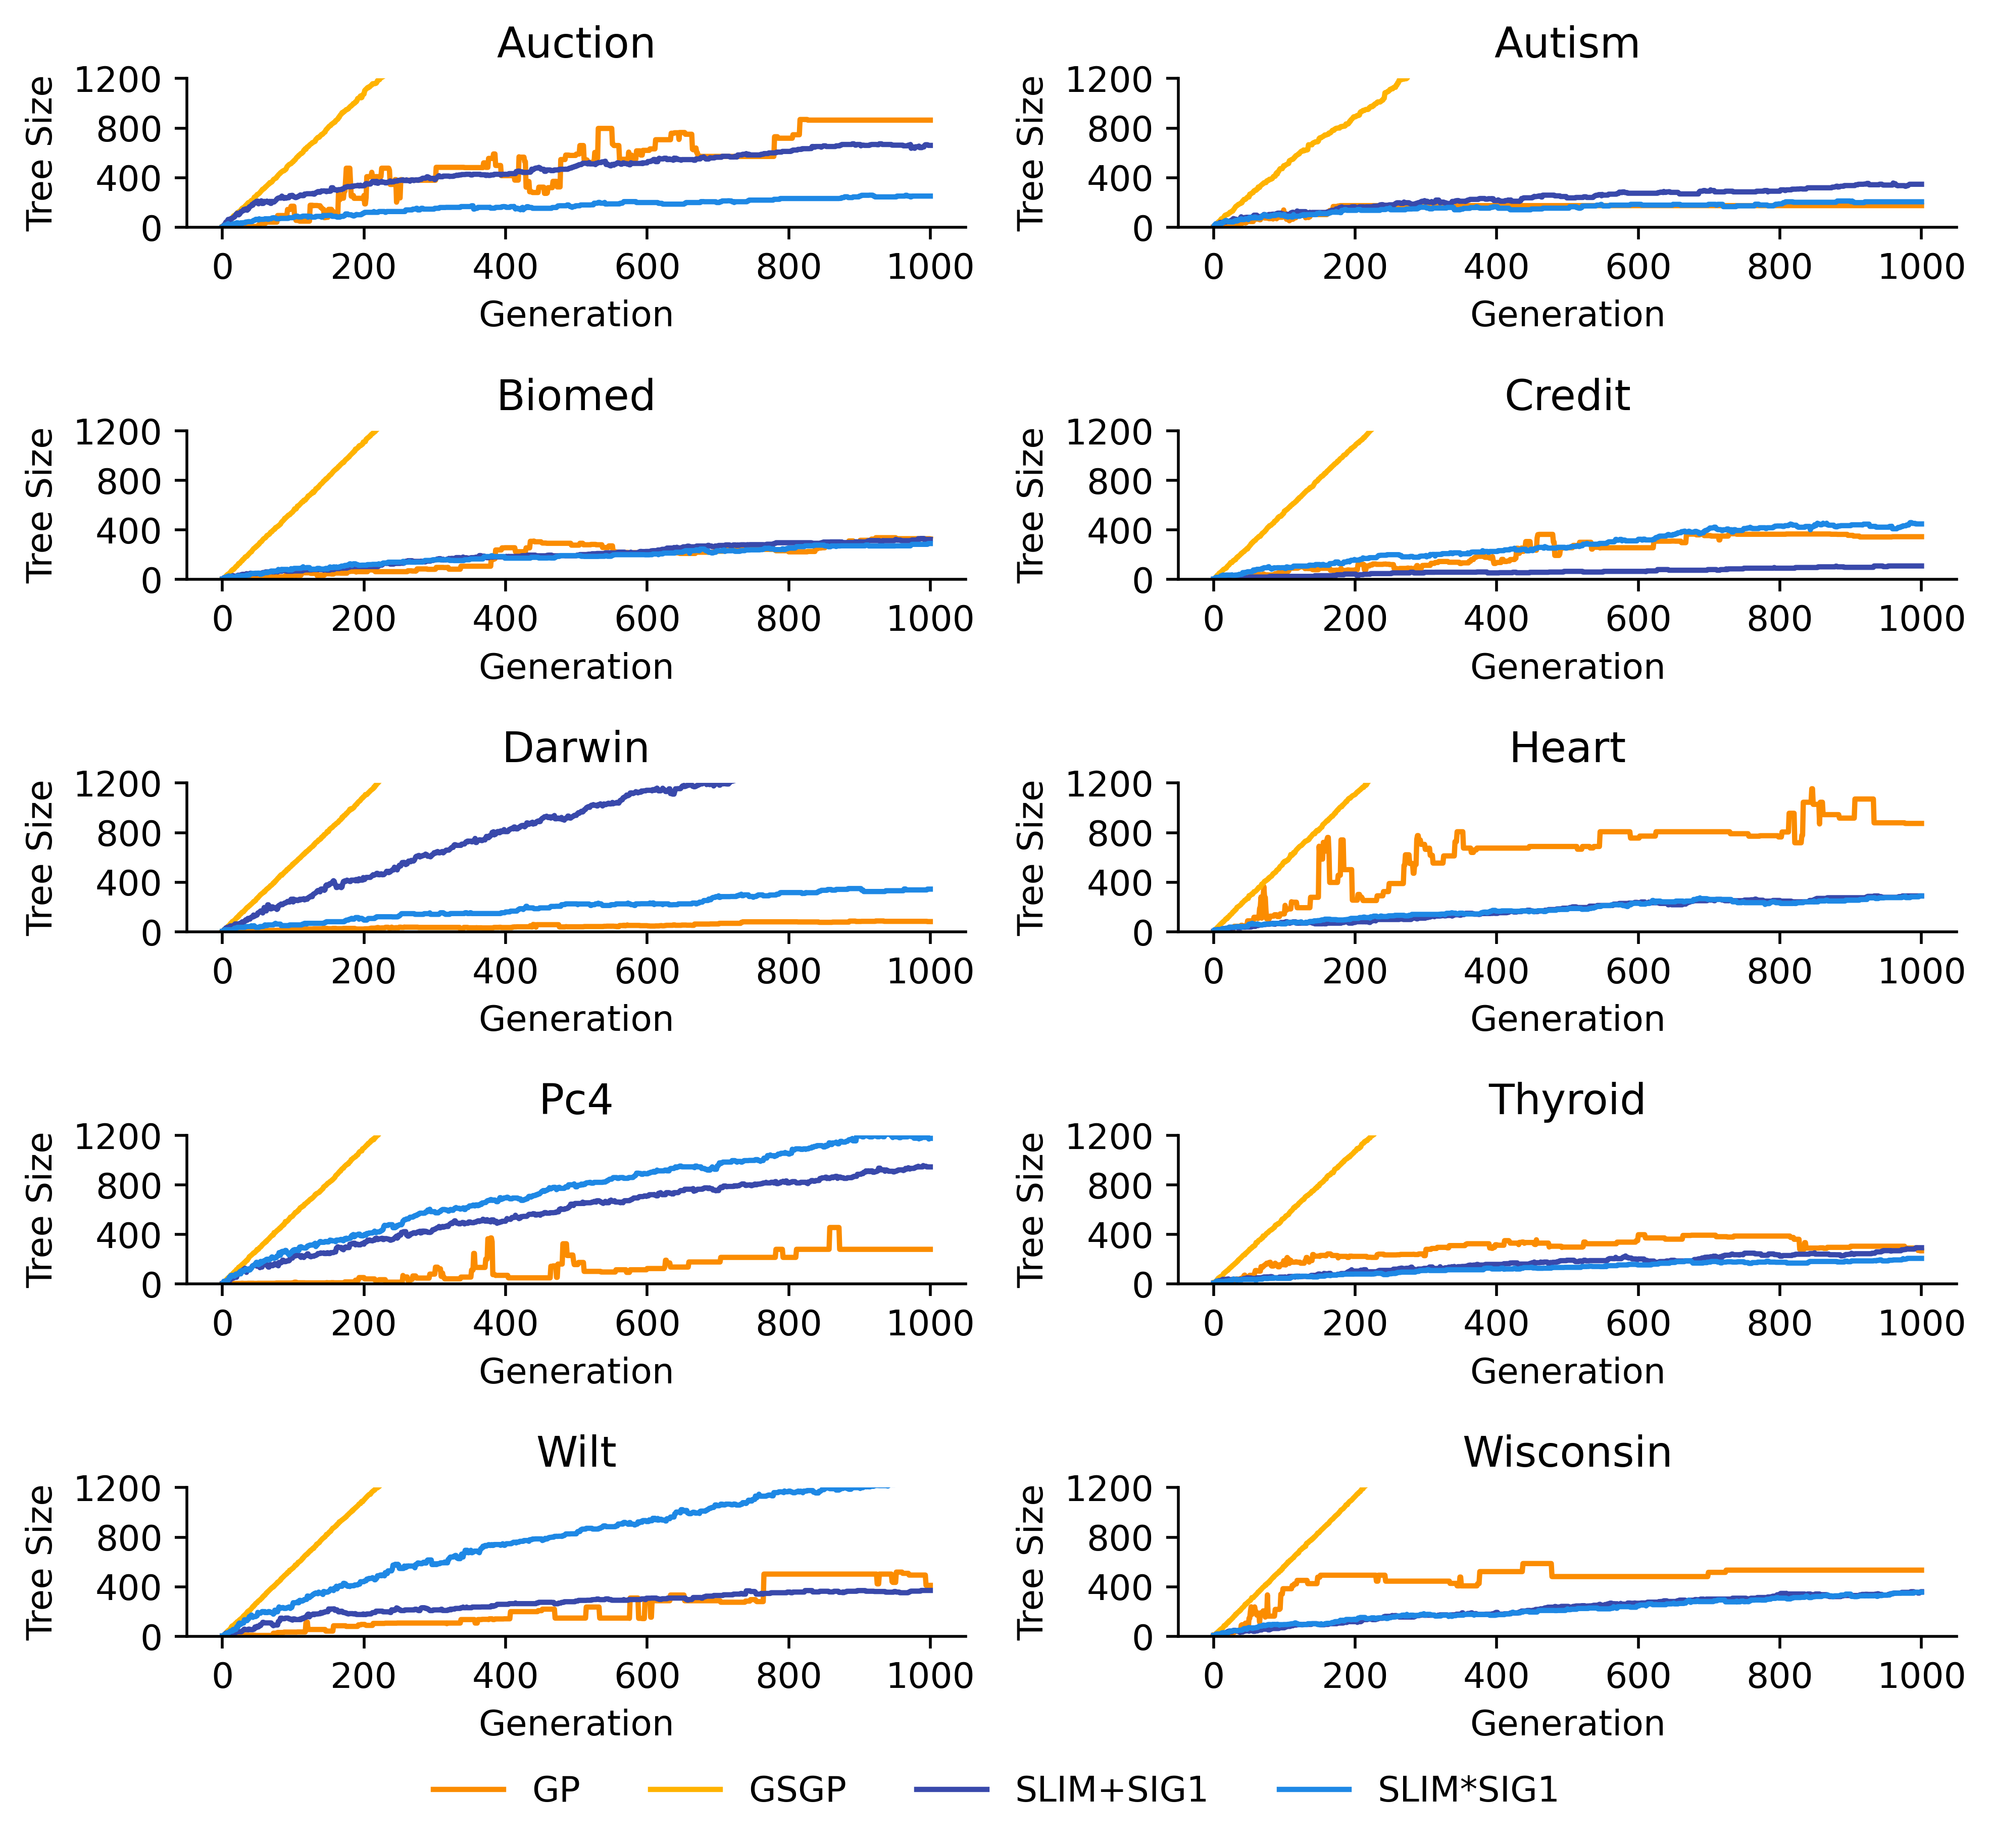
\includegraphics[width=\linewidth]{../Latex/Chapters/Figures/Results/comparison_tree_size_evolution.png}
    \caption{Tree Size Evolution by Algorithm}
    \label{fig:comparison_tree_size_evolution}
    \end{figure}
    
Figure \ref{fig:RQ_Comparison_performance_evolution} shows the median train and test RMSE of the elite individual
at a given generation.
We can see that the multiplication based version of SLIM-GSGP
struggles to learn from the training data in most of
the cases,
which is also reflected in the RMSE on the test
set. The addition based version of SLIM-GSGP, stdGP and GSGP
generally all adapt well to the training data,
whereas GSGP as expected adapts the best.
However, when it comes to the test set, we can see that GSGP and stdGP clearly struggle with overfitting 
on the Biomed and Credit datasets. Arguably GSGP also slightly overfits on the Heart and Wisconsin datasets.
SLIM+SIG1 in contrast always seems to generalize well. The test scores of the classifcation metrics can be found in figure
\ref{fig:RQ_Comparison_performance}.\\
For each dataset and evaluation metric we performed a pairwise
Wilcoxon rank sum test to determine weather the performances
of two different algorithms differ significantly at a 5\% level.
Based on the p-values we created a win-tie-loss table, which
can be found in Table \ref{tab:RQ_Comparison_wtl}.
A win/loss means that the performance of the algorithm is
significantly better/worse than the performance of the second algorithm.
A tie means that the performance of both algorithms are
not significantly different.
\ref{fig:RQ_Comparison_performance_evolution} already indicated that the multiplication based SLIM-GSGP version 
struggles to learn from the training data.

    \begin{table}[H]
        \centering
        \renewcommand{\arraystretch}{1.2}
        \caption{Win Tie Loss}
        \label{tab:RQ_Comparison_wtl}
    \begin{tabular}{lccccc}
\toprule
Algorithm & Accuracy & F1-Score & RMSE & ROC-AUC & Tree Size \\
\midrule
GP vs GSGP & 1-7-2 & 1-5-4 & 1-5-4 & 0-5-5 & 10-0-0 \\
GP vs SLIM*SIG1 & 9-0-1 & 9-0-1 & 7-2-1 & 5-2-3 & 4-2-4 \\
GP vs SLIM+SIG1 & 2-4-4 & 1-5-4 & 2-3-5 & 0-6-4 & 4-3-3 \\
GSGP vs SLIM*SIG1 & 9-1-0 & 9-0-1 & 9-0-1 & 6-3-1 & 0-0-10 \\
GSGP vs SLIM+SIG1 & 1-8-1 & 2-7-1 & 4-4-2 & 4-5-1 & 0-0-10 \\
SLIM*SIG1 vs SLIM+SIG1 & 0-1-9 & 0-1-9 & 0-1-9 & 1-2-7 & 6-1-3 \\
\bottomrule
\end{tabular}

        
    \end{table}
    
The win-tie-loss table confirms this, since the algorithm gets outperformed by all other algorithms on the majority of the datasets regarding all
performance metrics. The addition based version of SLIM-GSGP on the other hand, SLIM+SIG1, 
performs better than stdGP being able to outperform it on 6 out of 10 datasets regarding the fitness function RMSE on the test set and
only losing on 2 datasets. This also reflects in the accuracy, F1-Score and ROC-AUC. Regarding the tree size, SLIM+SIG1
performs significantly better than stdGP on 2 datasets and gets outperformed on 3 datasets, therefore we can say it is
kind of on par with stdGP regarding the tree size.\\
Performance-wise, SLIM+SIG1 performs better than GSGP on 2 datasets and worse on 4 datasets regarding the RMSE on the test set,
which can be considered respectable, since SLIM-GSGP outperforms GSGP on all datasets regarding the tree size.

    \begin{figure}[H]
    \centering
    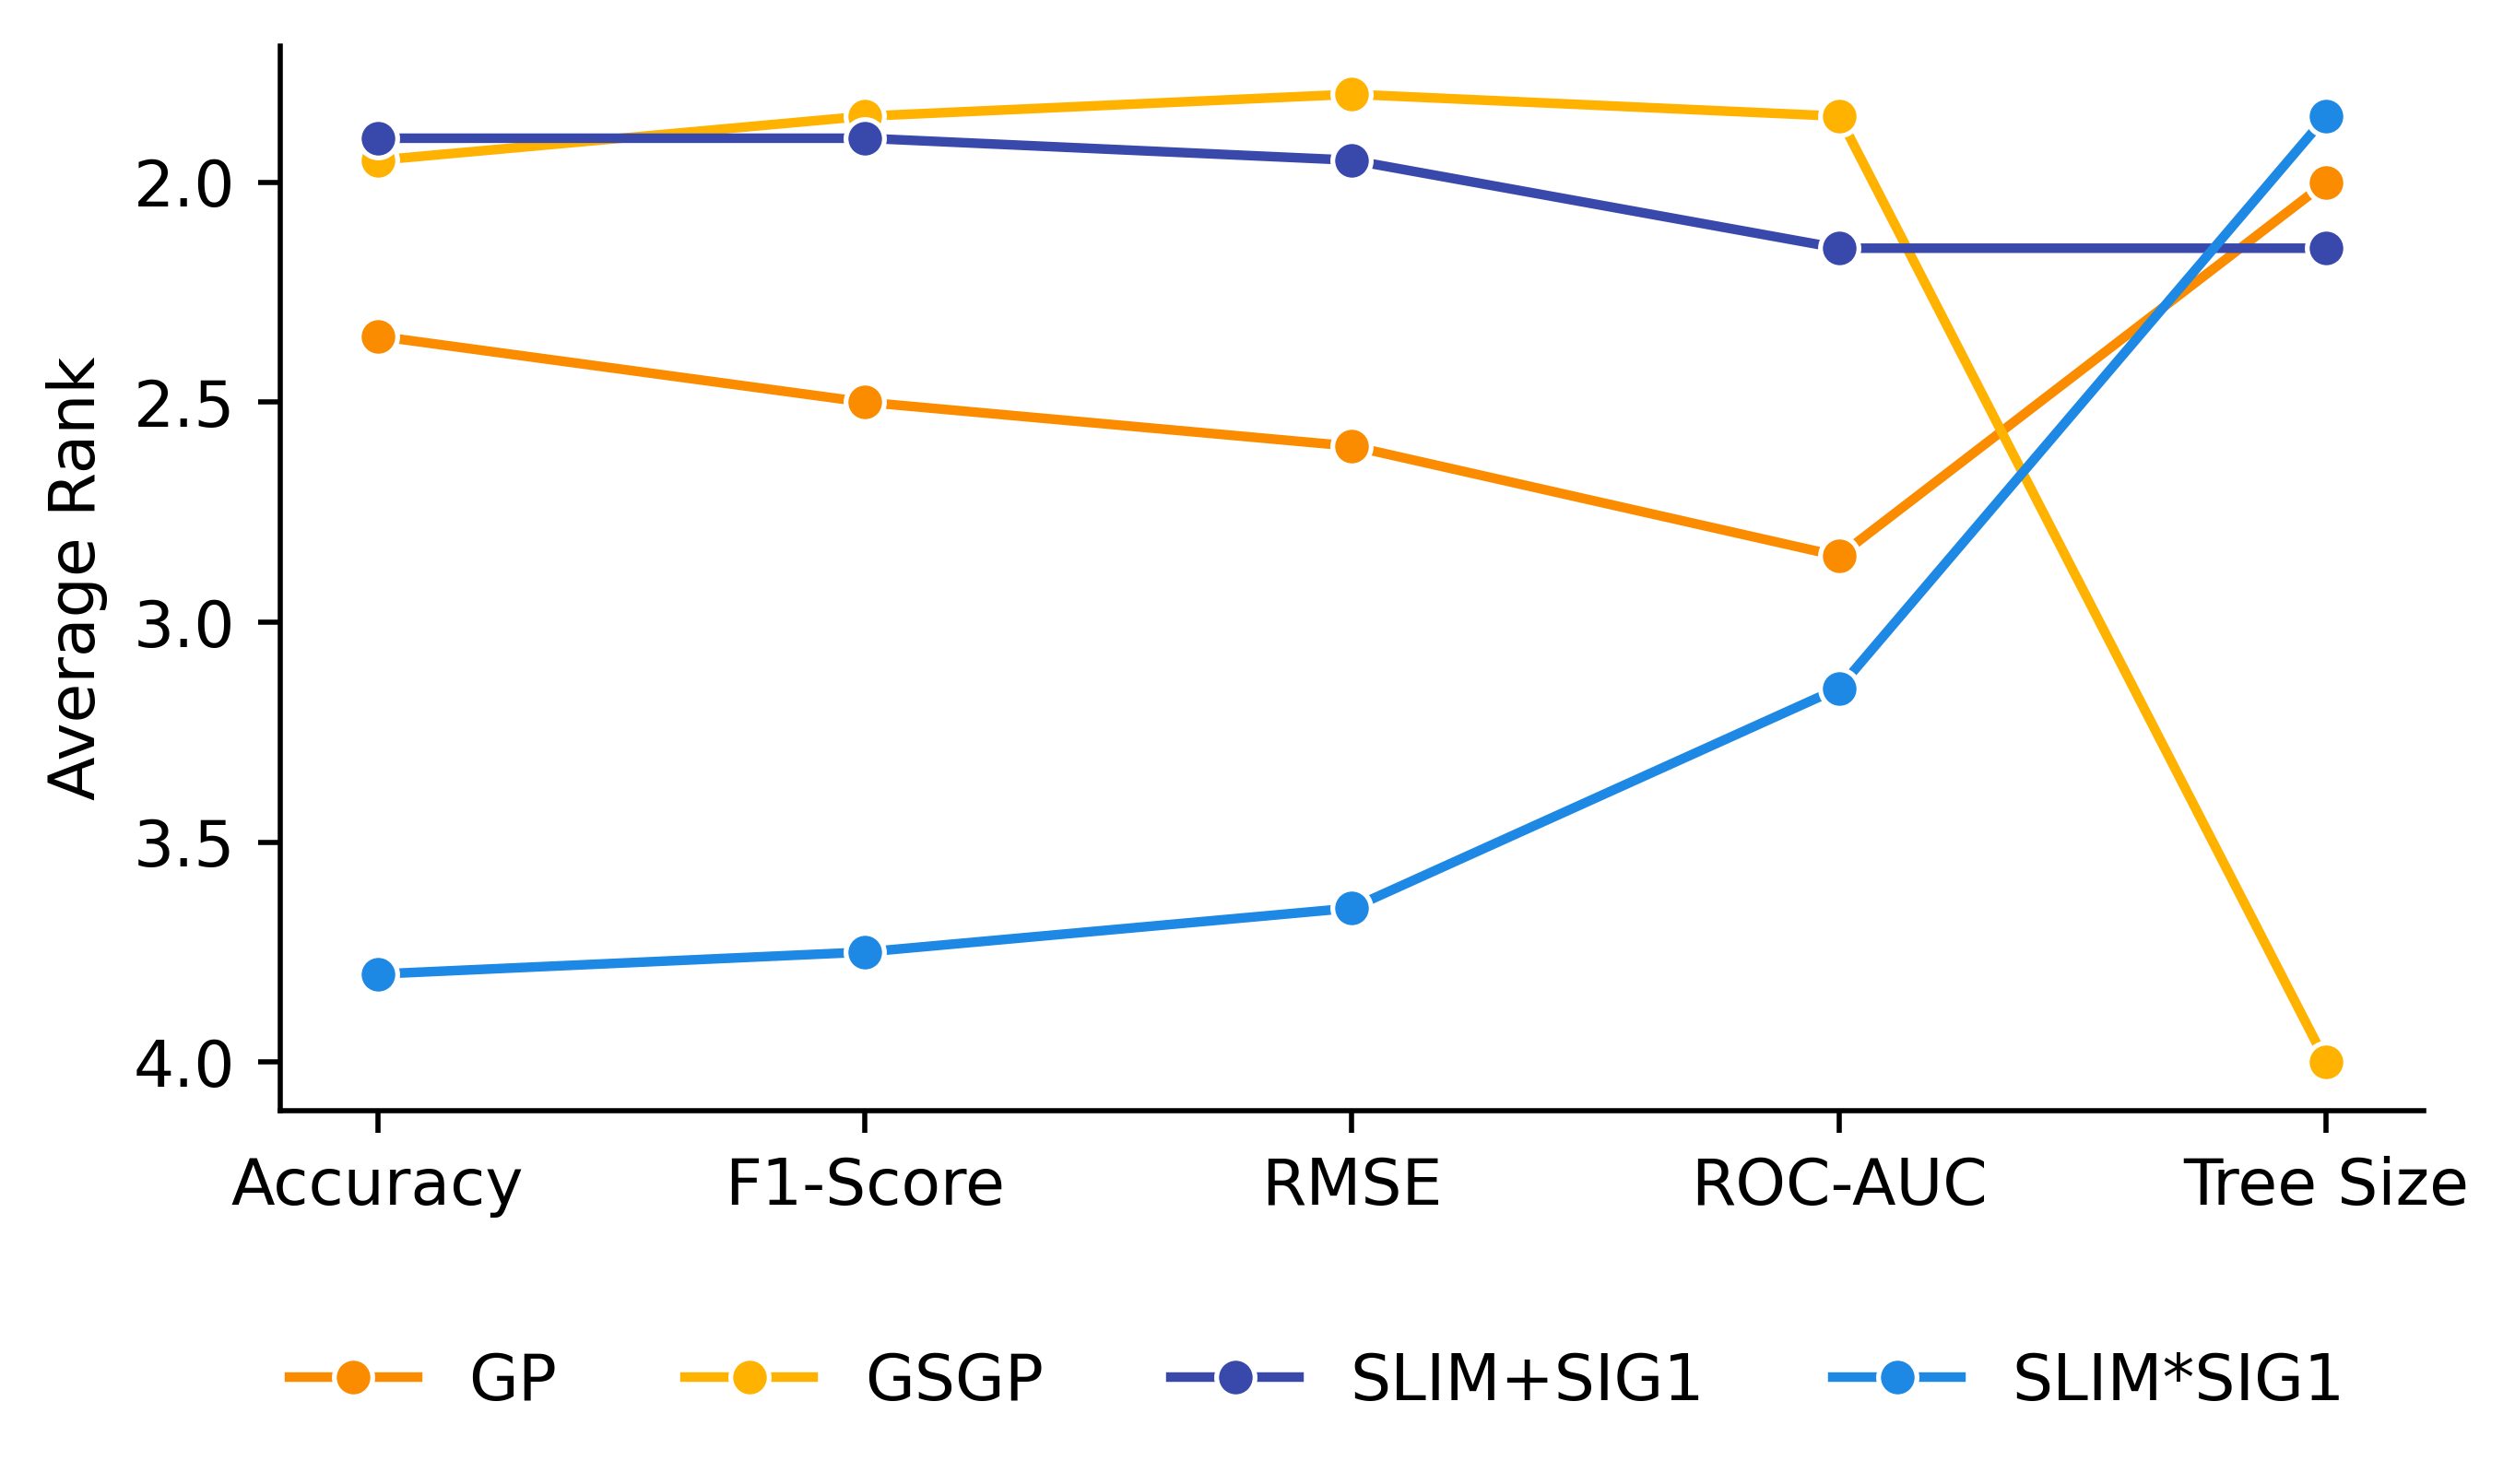
\includegraphics[width=\linewidth]{../Latex/Chapters/Figures/Results/RQ_Comparison_ranks.png}
    \caption{Ranks by Algorithm}
    \label{fig:RQ_Comparison_ranks}
    \end{figure}
    
\noindent Figure \ref{fig:RQ_Comparison_ranks} shows the mean ranks of the algorithms across
datasets based on the win-tie-loss table.
For each dataset the ranks of the algorithms are calculated
as $Rank = 1 + 0.5 \cdot N_{Ties} + 1
\cdot N_{Losses}$.
As a consequence a rank of 1 means that the
algorithm outperformed all other algorithms,
whereas a rank of 4 means that the algorithm was
outperformed by all other algorithms. 
As the comparison of the ranks further demonstrates, SLIM+SIG1 performs nearly as well as GSGP regarding the performance metrics,
while being able to produce individuals of similar size to stdGP individuals.\\
Table \ref{tab:RQ_Comparison_friedman} shows the results of the Friedman test, that
was performed to determine if the
differences regarding the ranks are significant, which they are forall of the metrics.


    \begin{table}[H]
        \centering
        \renewcommand{\arraystretch}{1.2}
        \caption{p-Values of the Friedman Test}
        \label{tab:RQ_Comparison_friedman}
    \begin{tabular}{lcc}
\toprule
Metric & P-Value & Significant \\
\midrule
Accuracy & 0.001591 & Yes \\
F1-Score & 0.002385 & Yes \\
RMSE & 0.001817 & Yes \\
ROC-AUC & 0.181558 & No \\
Tree Size & 0.000152 & Yes \\
\bottomrule
\end{tabular}

        
    \end{table}
    
\subsubsection{Interpretation}
This comparative analysis evaluates how SLIM-GSGP performs regarding prediction quality and tree size compared to GSGP and stdGP.
While SLIM*SIG1 shows poor overall performance SLIM+SIG1 achieves a strong trade-off:
it performs comparably to GSGP in terms of prediction quality, sometimes better,
sometimes slightly worse depending on the dataset, while generating significantly smaller individuals.
In terms of tree size, SLIM+SIG1 models are consistently close to those produced by stdGP and drastically smaller than GSGP individuals.
GSGP still achieves the best RMSE on the test set in several cases, which often translates into better F1-Score and ROC-AUC.
However, on datasets prone to overfitting, SLIM+SIG1 can outperform GSGP thanks to its better generalization capability, 
likely due to the regularizing effect of deflation mutation.
Overall, SLIM-GSGP preserves much of the predictive power of
GSGP while producing models as small and interpretable as those from stdGP, therefore successfully addressing
the performance-complexity trade-off in symbolic regression-based classification.

%
    \begin{figure}[H]
    \centering
    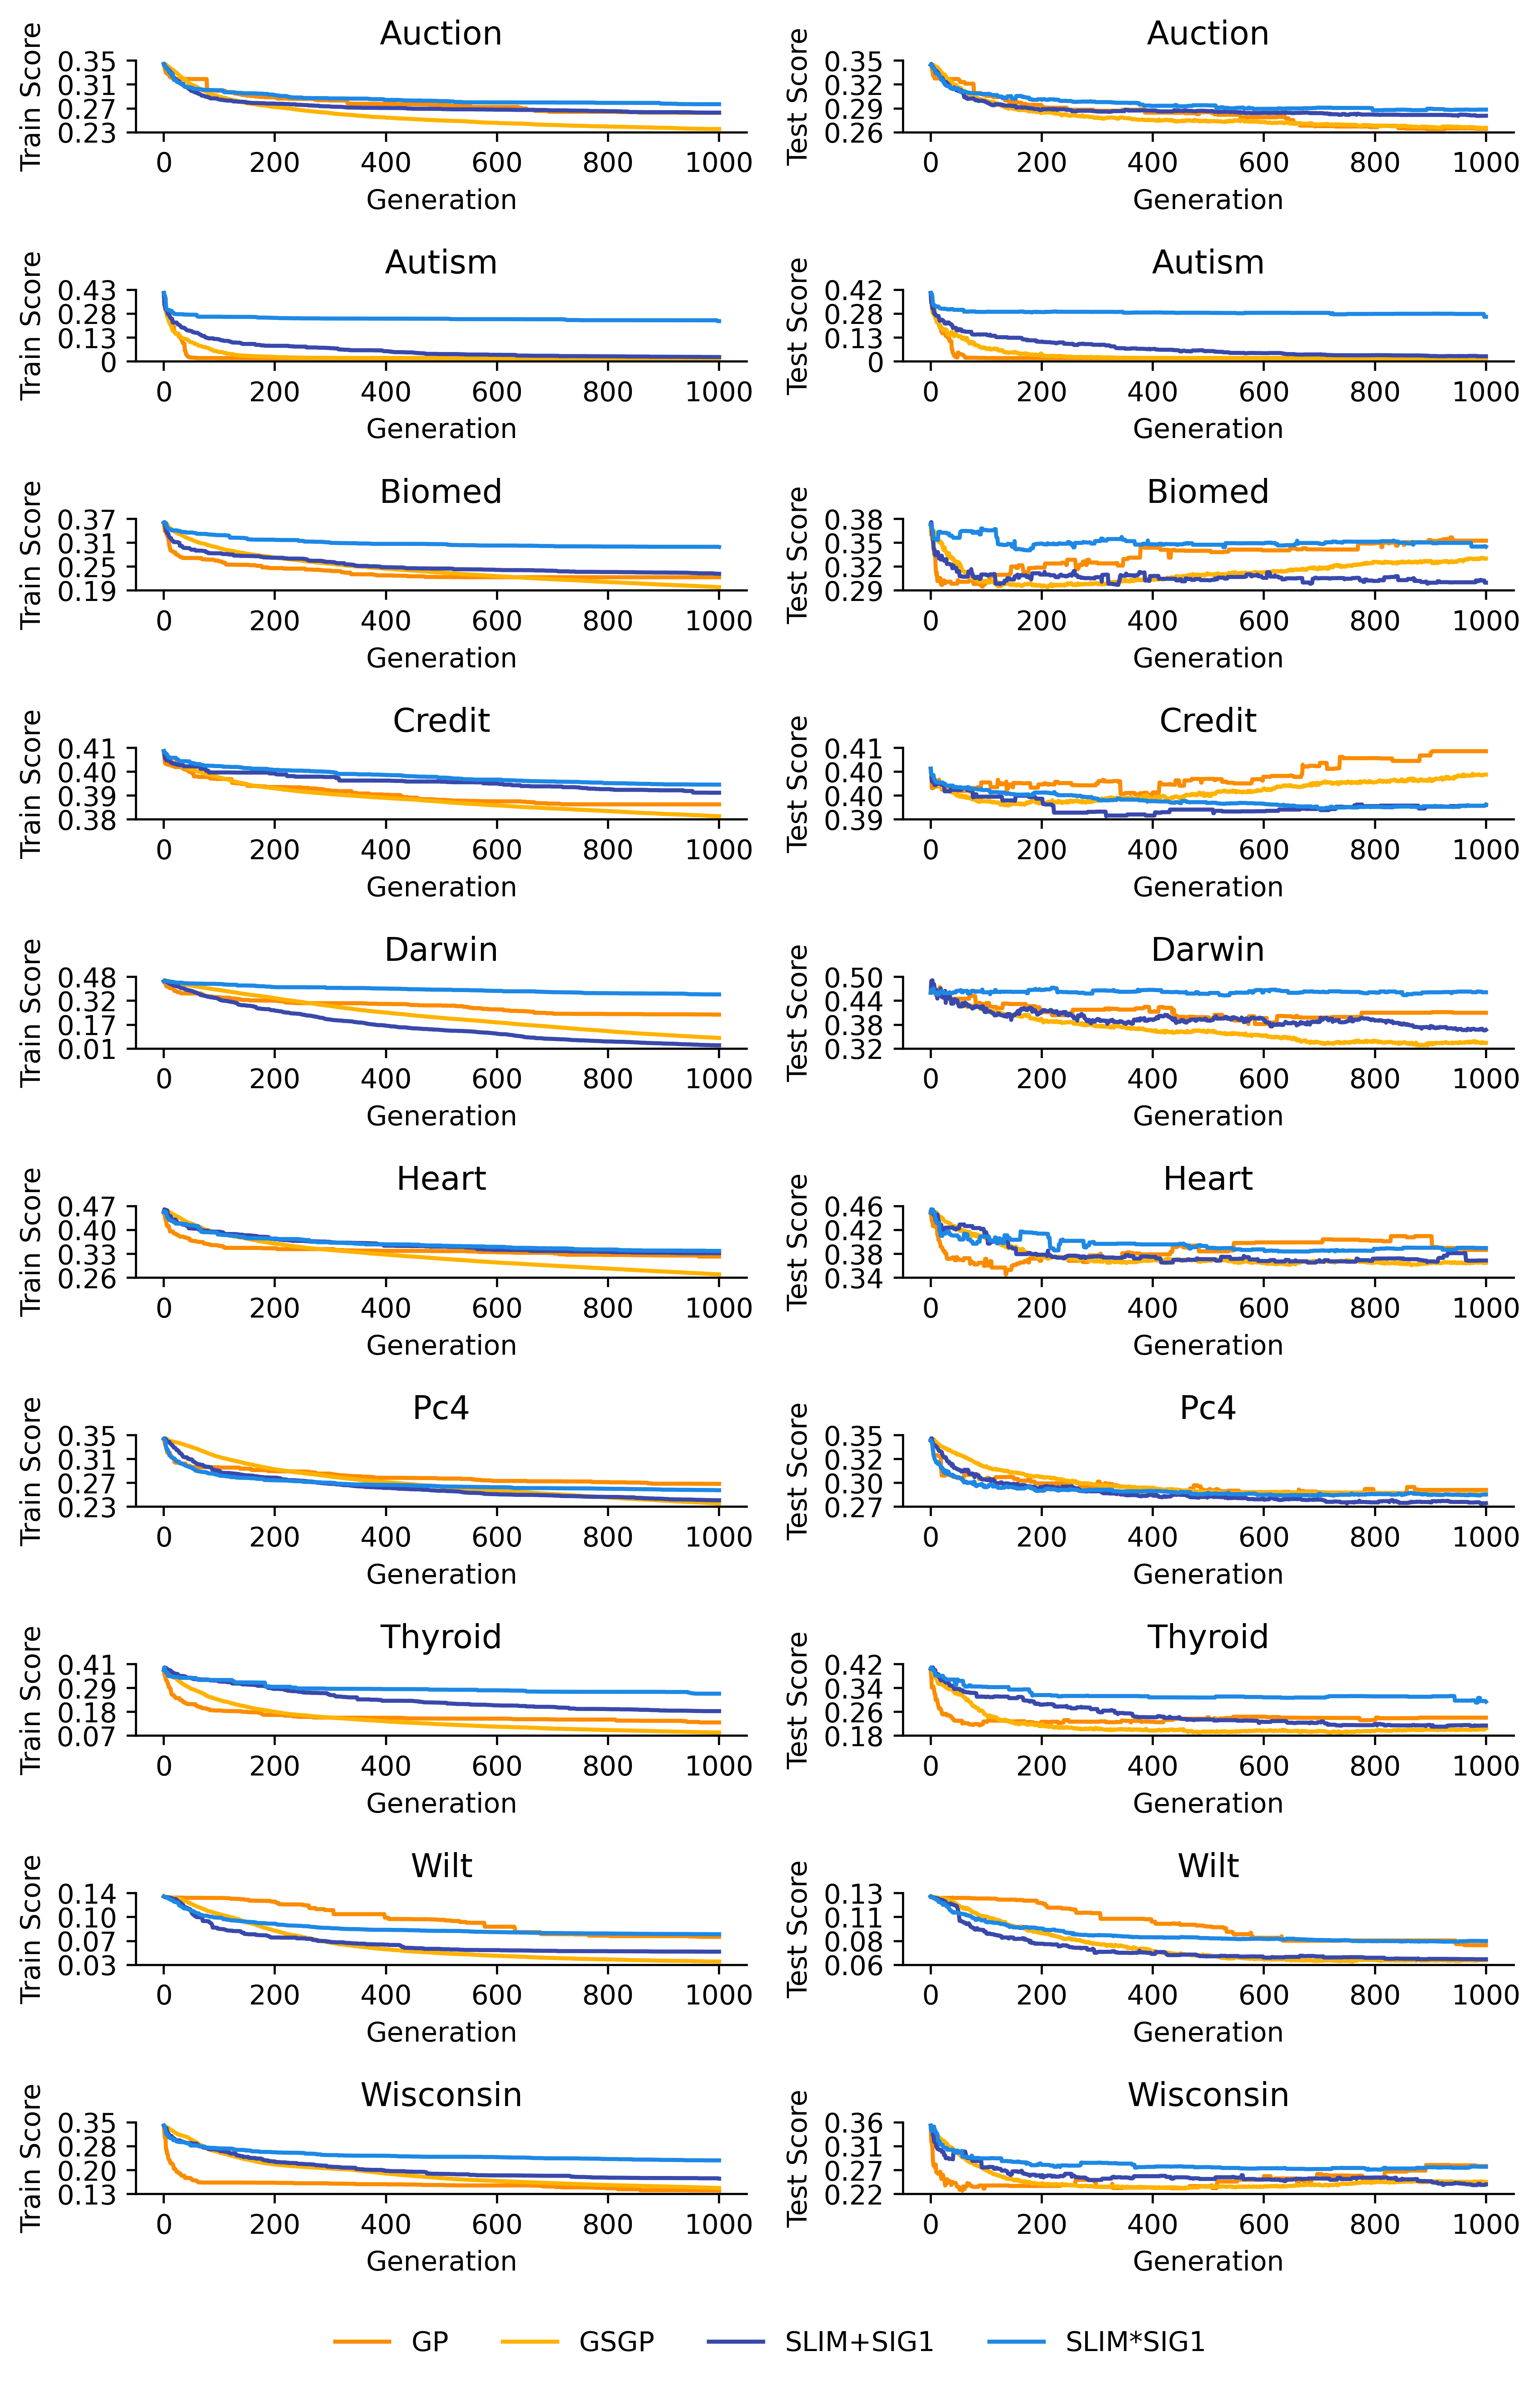
\includegraphics[width=\linewidth]{../Latex/Chapters/Figures/Results/comparison_performance_evolution.png}
    \caption{Performance Evolution by Algorithm}
    \label{fig:comparison_performance_evolution}
    \end{figure}
    
%
    \begin{figure}[h]
    \centering
    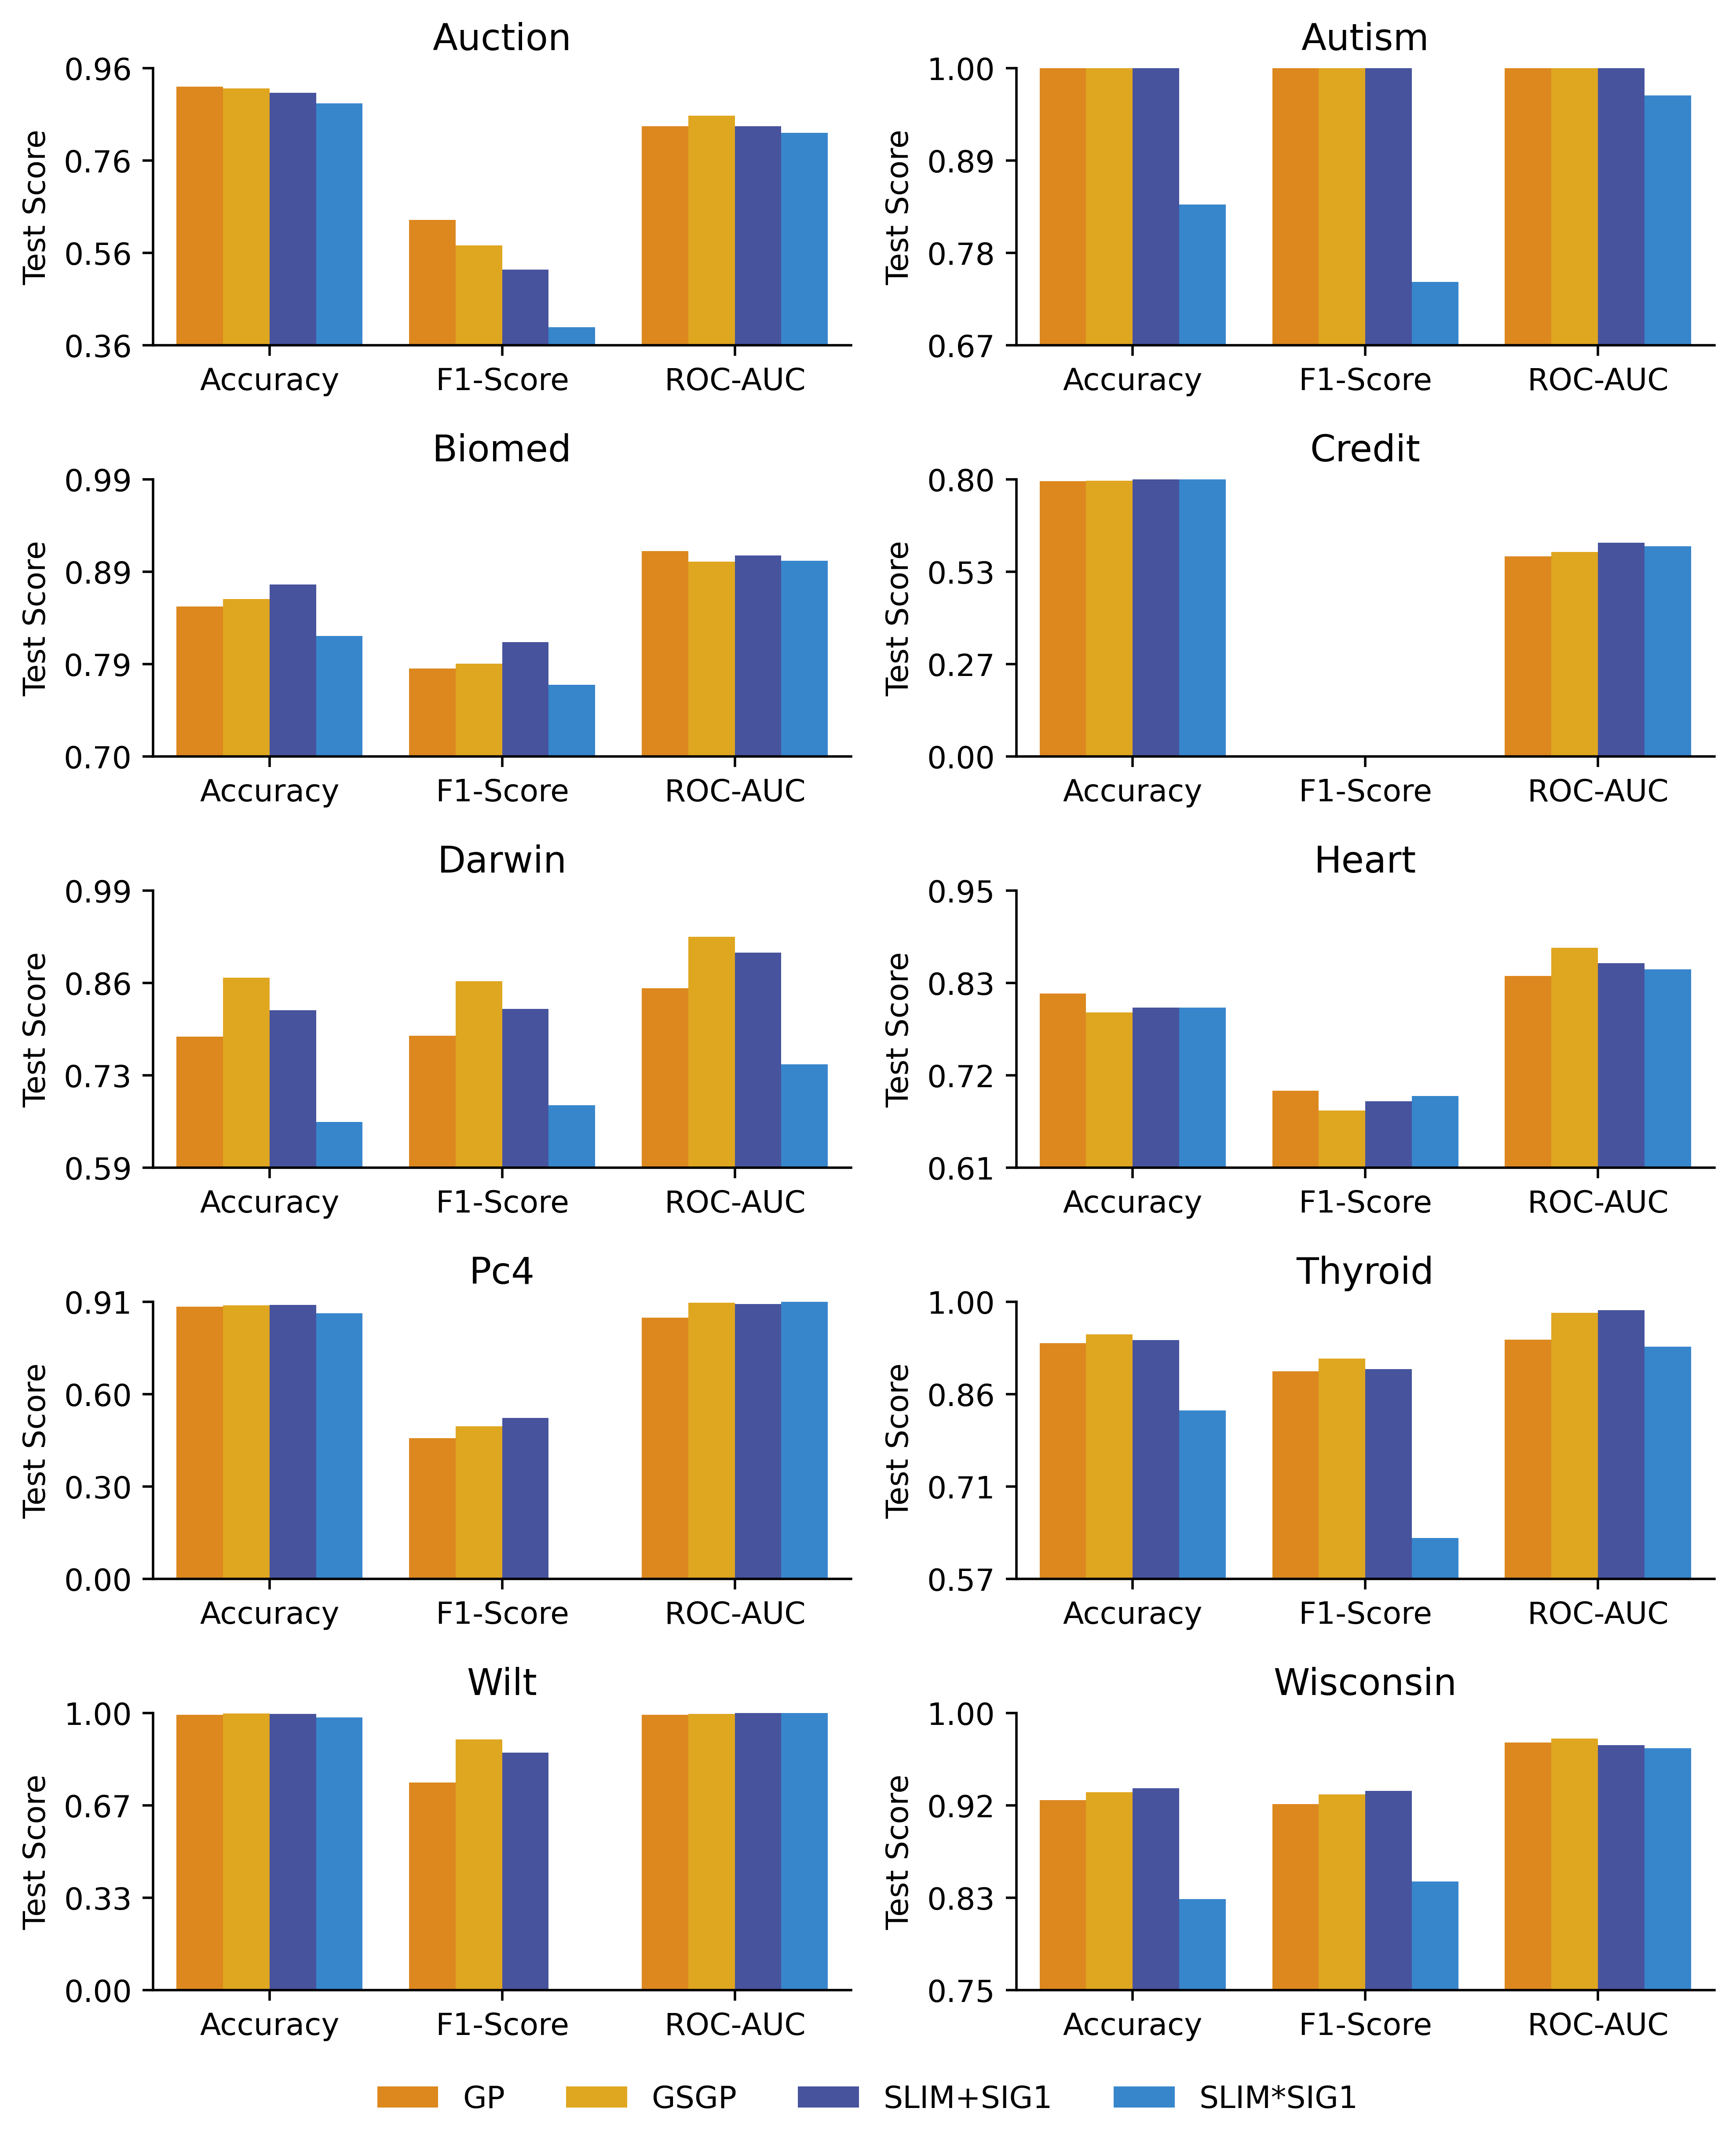
\includegraphics[width=\linewidth]{../Latex/Chapters/Figures/Results/comparison_performance.png}
    \caption{Performance by Algorithm}
    \label{fig:performance}
    \end{figure}
    

\section{Conclusion and Future Work}
\label{cha:conclusion}

\subsection{Conclusion}
This study investigated how different design decisions affect performance 
and complexity in symbolic regression-based genetic programming with GSO for binary classification
and introduced the SLIM-GSGP algorithm for this purpose.
We addressed three main aspects through a series of structured experiments:
First, we studied the impact of fitness function choice on model performance for GSGP.
Second, we analyzed how the inflation rate and mutation upper step influence the performance-complexity trade-off in SLIM-GSGP.
Third, we evaluated how SLIM-GSGP compares to GSGP and stdGP in terms of prediction quality and tree size.
In \textbf{Experiment 1}, 
we studied the impact of different fitness functions on the performance and tree size of traditional GSGP.
We chose traditional GSGP over SLIM-GSGP for this experiment, since
traditional GSGP had been used successfully in previous work,
and we wanted to keep the hyperparameter settings consistent with those studies.
We argue that the results of this experiment are also applicable to SLIM-GSGP in the context of binary classification,
as both algorithms are based on the GSO defined for regression problems, and the exploration behavior 
of the search space is similar.\\
Our implementation of GSGP used symbolic regression-based individuals.
We compared two types of fitness functions: regression-based (RMSE and WRMSE) and classification-based (accuracy and F1-Score).
The regression-based fitness functions required a 
logistic activation function to transform the output of the symbolic regression-based individuals into a probability between 0 and 1.
The hard classification of the individual returned by the algorithm was then enabled by applying a threshold at 0.5 to 
the output of the logistic function.
The classification-based fitness functions used a HSF directly on the output of the symbolic regression-based individuals,
resulting in a hard classification at the evaluation stage already.\\
The results showed that regression-based fitness functions like RMSE and WRMSE, 
when combined with the logistic function, provide smoother feedback during optimization, 
which leads to better performance. Classification-based functions like accuracy and F1-Score, 
which rely on the Heaviside Step Function, offer only discrete feedback, 
making improvements less frequent and causing the search process to stagnate. 
This also results in stepwise growth in model size. 
While regression-based functions tend to produce larger trees, their superior optimization performance makes them preferable.\\
\textbf{Experiment 2} focused on the inflation rate in SLIM-GSGP and how it influences the trade-off between performance and complexity.
We choose two versions of SLIM-GSGP: 
one with addition-based deflation mutation (SLIM+1) and one with multiplication-based deflation mutation (SLIM*1).
To enable the algorithm for binary classification, 
we applied a logistic activation function to the output of the symbolic regression-based individuals, 
and used the RMSE as the fitness function.\\
The results showed that a higher inflation rate consistently leads to larger individuals, 
while a lower inflation rate helps reduce size. In terms of generalization, 
there is no clear trend, but in many cases, 
lower inflation rates produced smaller individuals with similar or even better test performance. 
This suggests that the deflation mutation not only helps control size but also acts as a form of regularization. 
Using a weighted Euclidean distance based on normalized RMSE and tree size, 
we were able to identify configurations that represent a good trade-off.\\
\textbf{Experiment 3} compared SLIM-GSGP to traditional GSGP and stdGP.
We applied a logistic activation function to the output of the symbolic regression-based individuals, and used the RMSE as the fitness function.
To enable the models returned by the algortihms for binary classification,
we applied a threshold at 0.5 to the output of the logistic function.\\ 
The addition-based SLIM version (SLIM+SIG1) performed nearly as well as GSGP, 
and in some cases generalized better. At the same time, the models were much smaller, 
often similar in size to those from stdGP. While the multiplication-based SLIM version struggled to learn effectively, 
SLIM+SIG1 achieved a good balance between complexity and performance.\\
The results of this study show that it is possible to build accurate and interpretable models using Genetic Programming. 
This is especially relevant in areas where model transparency is important, 
such as healthcare or finance. 
SLIM-GSGP offers a way to retain much of the predictive quality of GSGP while producing models that are simpler and easier to understand. 
This could make symbolic regression-based models more applicable in real-world settings where interpretability is often a requirement.
\subsection{Future Work}
Future work could focus on enhancements of the fitness function.
Combining the distance-based fitness functions with the ROC-AUC metric as a multi-objective fitness function
in combination with a logistic activation function could
be an interesting approach. It would enable the algorithm to train for
separating the classes, while being aware of a hard classification threshold at 0.5.\\
Also the usage of multi-objective fitness functions, directly trading off size
and performance, could be a promising research topic.\\
Furthermore the application of SLIM-GSGP
for multi-class classification problems, by evolving one-versus-all classifiers, seems like
an intriguing prospect.\\
Lastly, Moraglio \cite{Moraglio2012} defined GSO for both regression and classification problems, whereas we have not found any work
that focused on the GSOs defined for classification problems. So instead of evolving symbolic regression-based individuals,
the GSOs defined for classification problems could be used to evolve individuals that are represented by classification rules
or decision trees. One of the main reasons why the majority of research for binary classification has been focused
on symbolic regression-based individuals is the historical success of GSGP 
on regression problems. A systematic comparison of regression-based and classification-based GSO 
could lead to interesting insights.





%%
%% The acknowledgments section is defined using the "acks" environment
%% (and NOT an unnumbered section). This ensures the proper
%% identification of the section in the article metadata, and the
%% consistent spelling of the heading.
\begin{acks}
To Robert, for the bagels and explaining CMYK and color spaces.
\end{acks}

%%
%% The next two lines define the bibliography style to be used, and
%% the bibliography file.
\bibliographystyle{ACM-Reference-Format}
\bibliography{sample-base}


%%
%% If your work has an appendix, this is the place to put it.
\appendix

\section{Results}
\subsection{Experiment 1: The impact of different fitness functions}
\label{app:exp1}


    \begin{figure}[H]
    \centering
    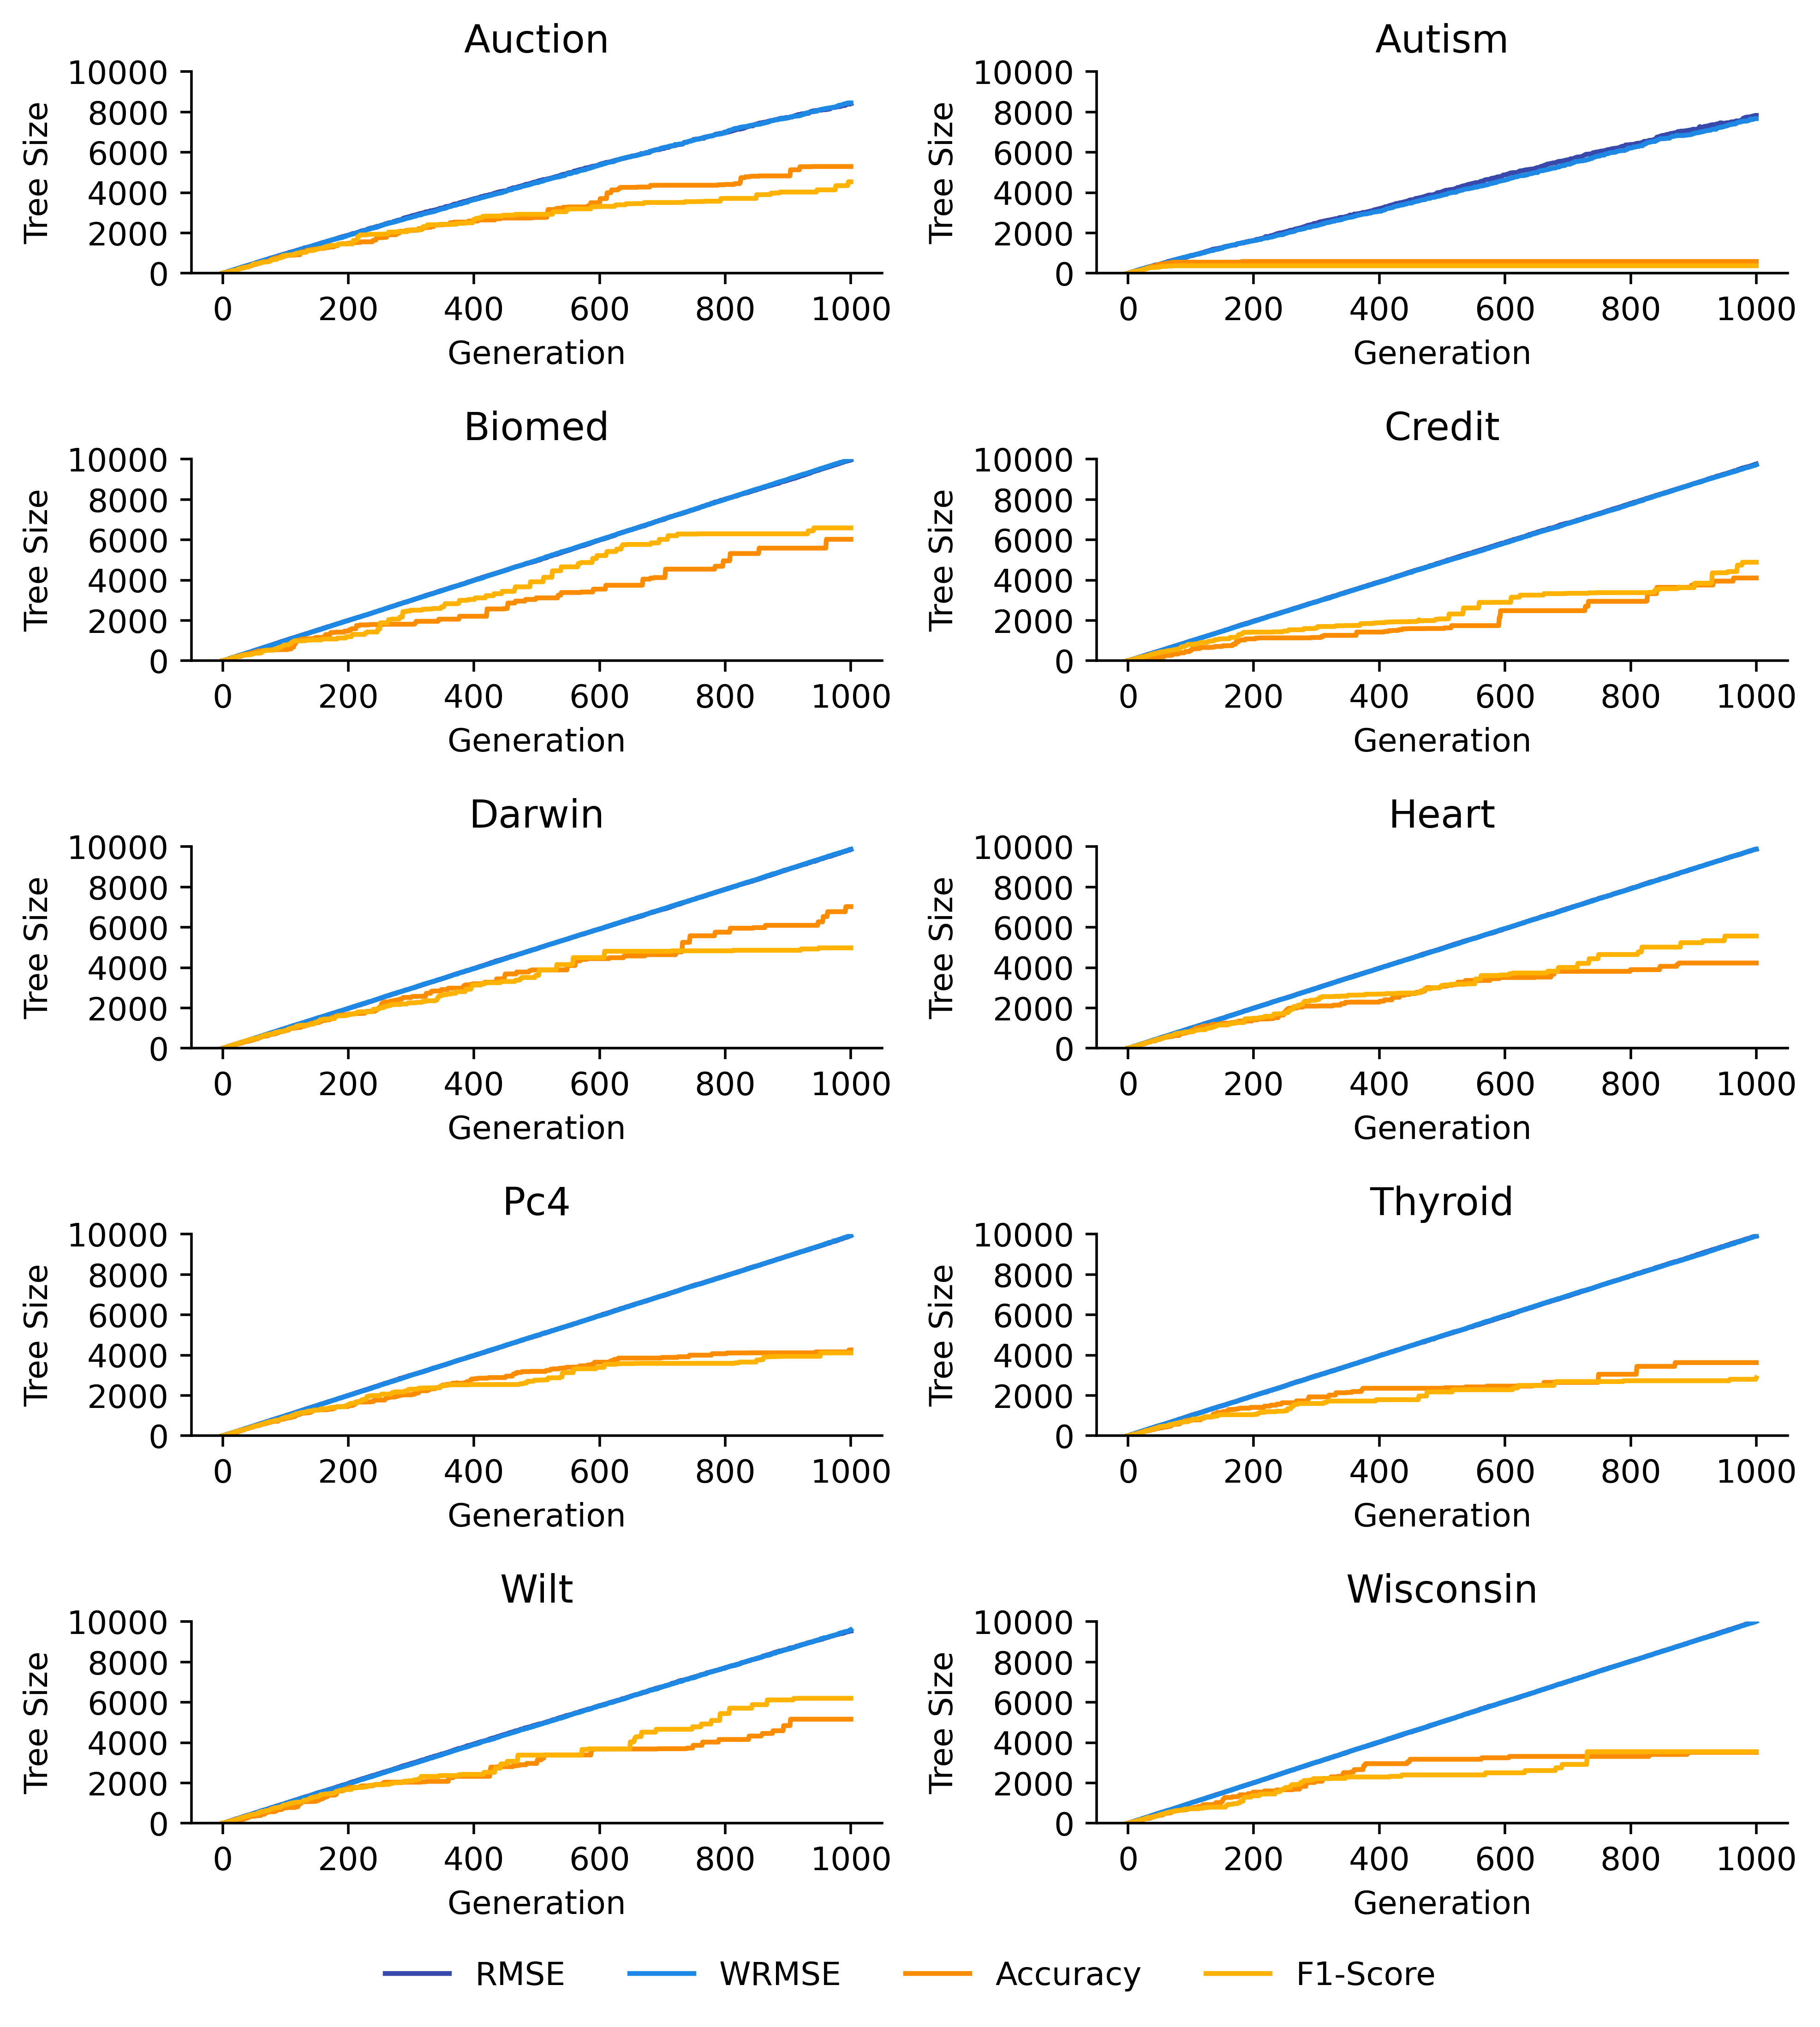
\includegraphics[width=\linewidth]{../Latex/Chapters/Figures/Results/RQ_Fitness_tree_size_evolution.png}
    \caption{Tree Size Evolution by Fitness Function}
    \label{fig:RQ_Fitness_tree_size_evolution}
    \end{figure}
    
\newpage

    \begin{figure}[H]
    \centering
    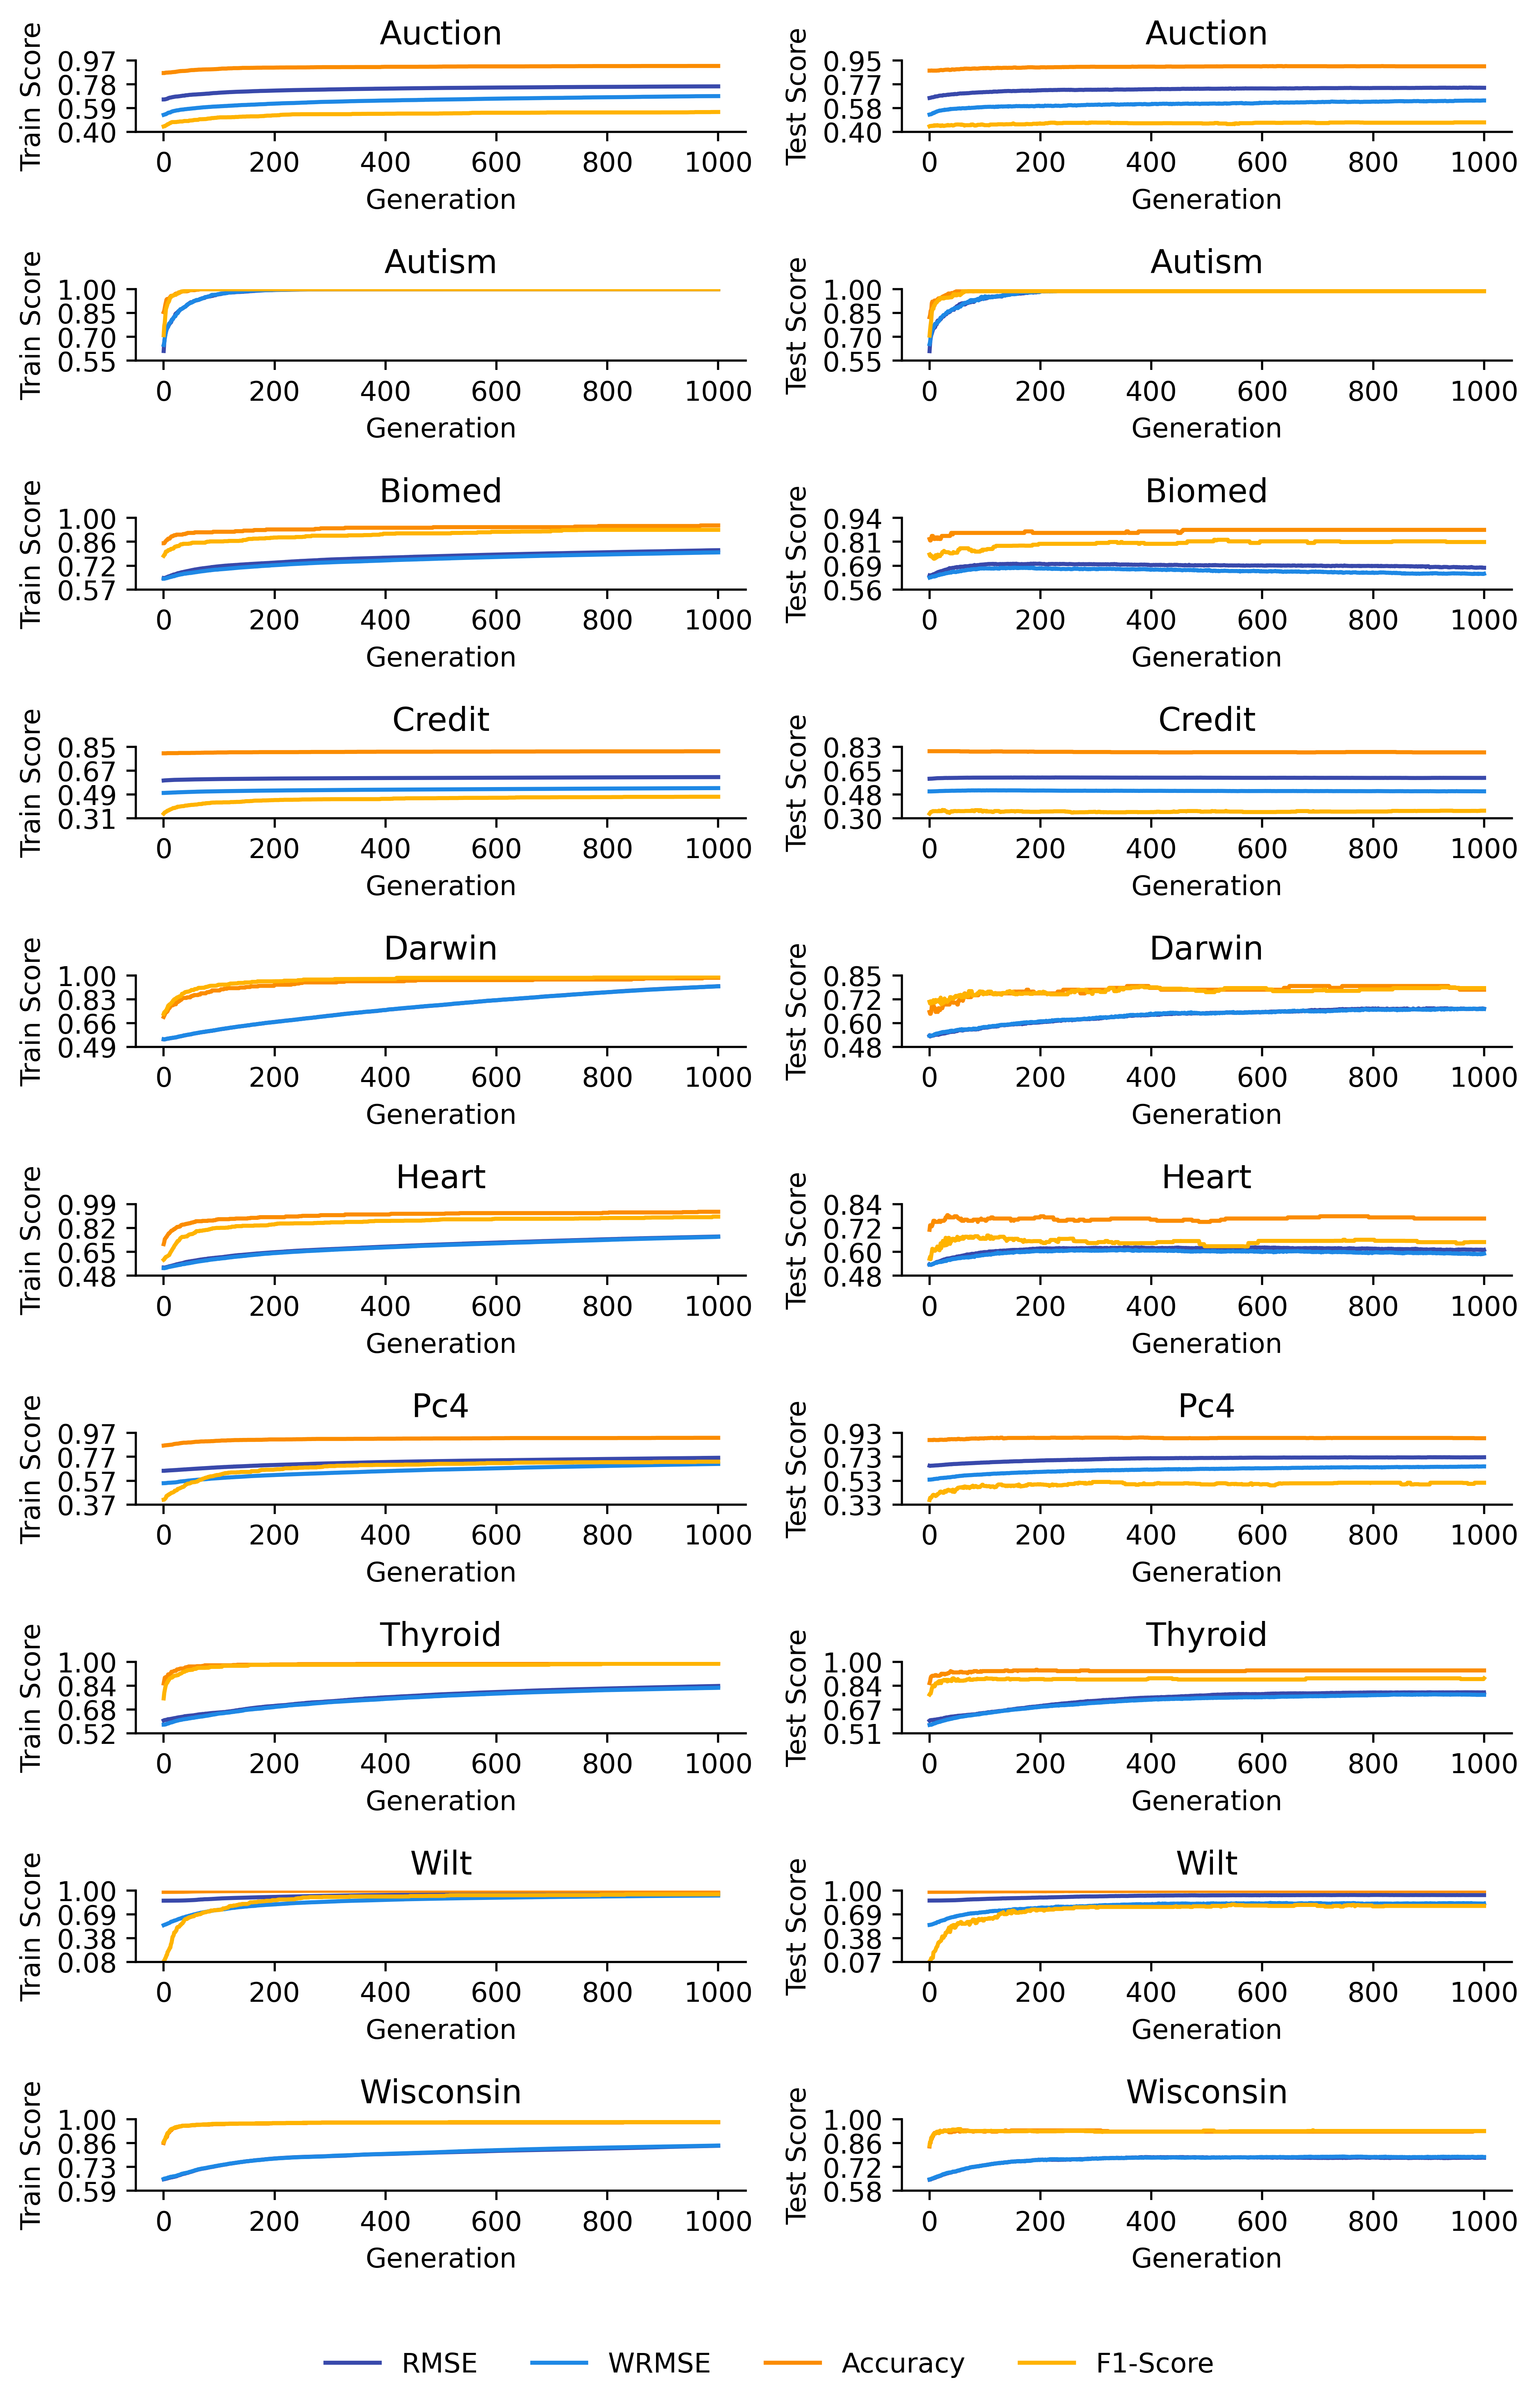
\includegraphics[width=\linewidth]{../Latex/Chapters/Figures/Results/RQ_Fitness_performance_evolution.png}
    \caption{Performance Evolution by Fitness Function}
    \label{fig:RQ_Fitness_performance_evolution}
    \end{figure}
    
\newpage

    \begin{figure}[H]
    \centering
    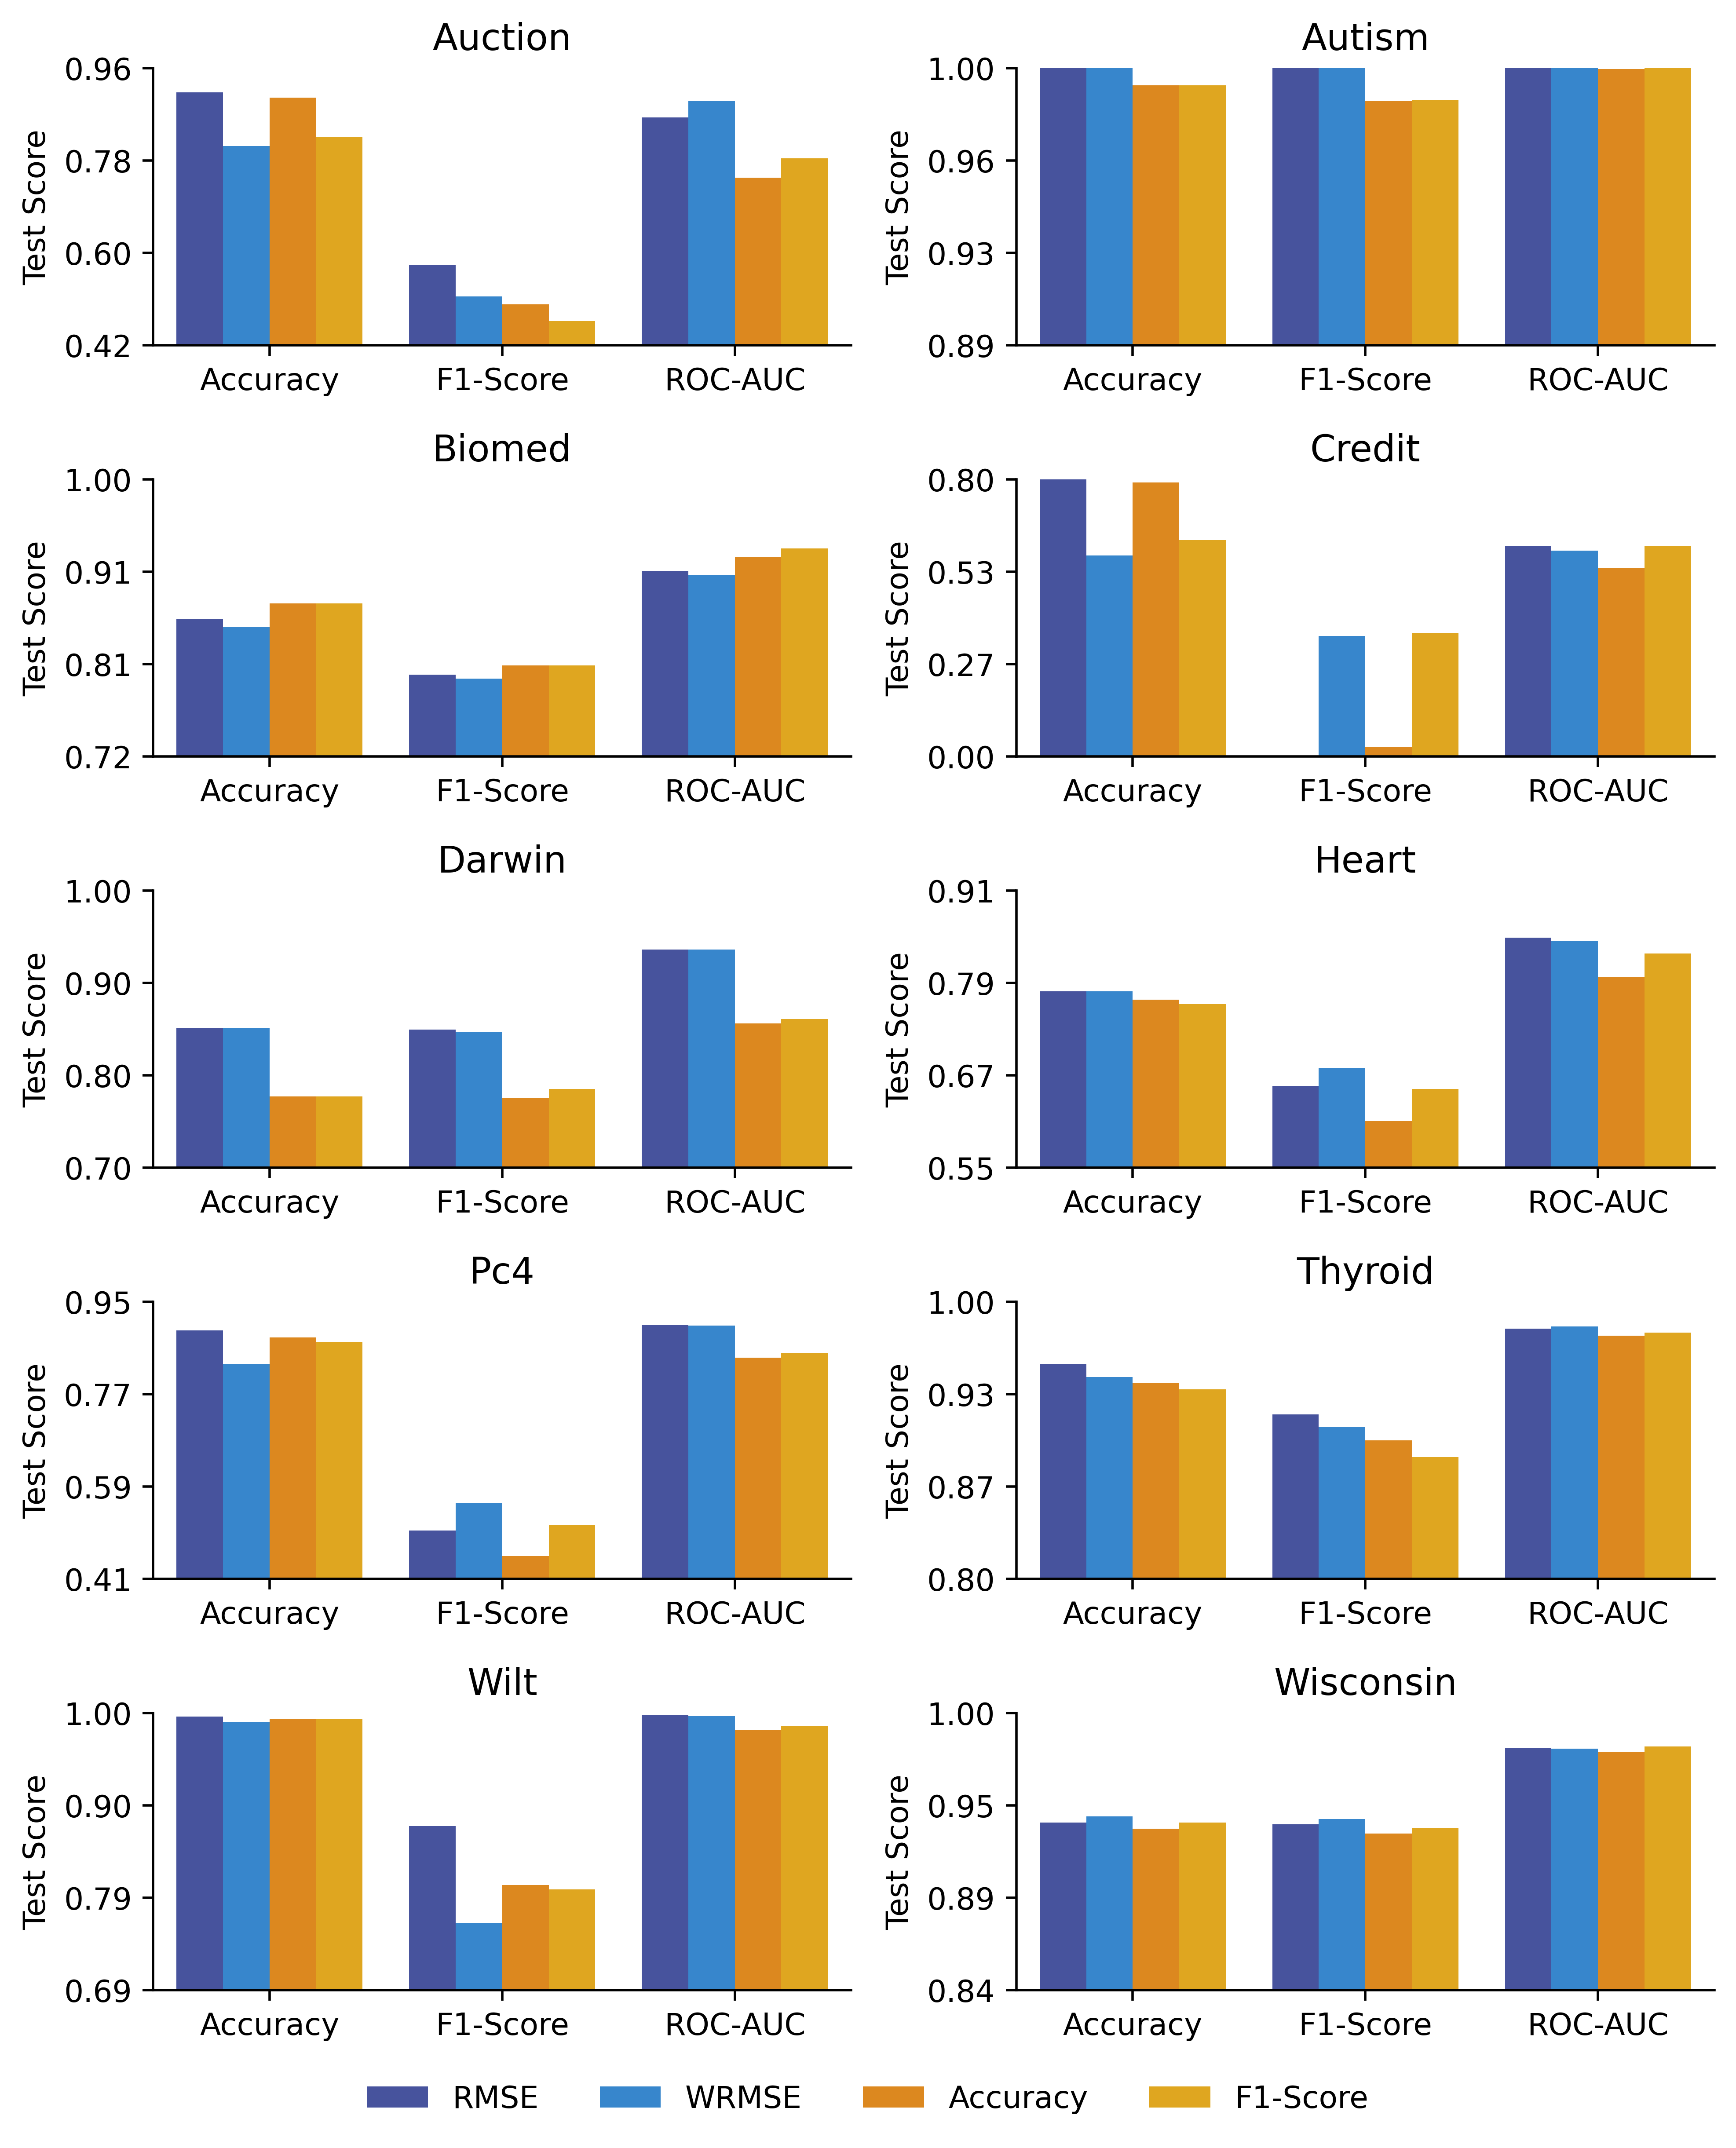
\includegraphics[width=\linewidth]{../Latex/Chapters/Figures/Results/RQ_Fitness_performance.png}
    \caption{Performance by Fitness Function}
    \label{fig:RQ_Fitness_performance}
    \end{figure}
    
\subsection{Experiment 2: The impact of the inflation rate}
\label{app:exp2}

    \begin{figure}[H]
    \centering
    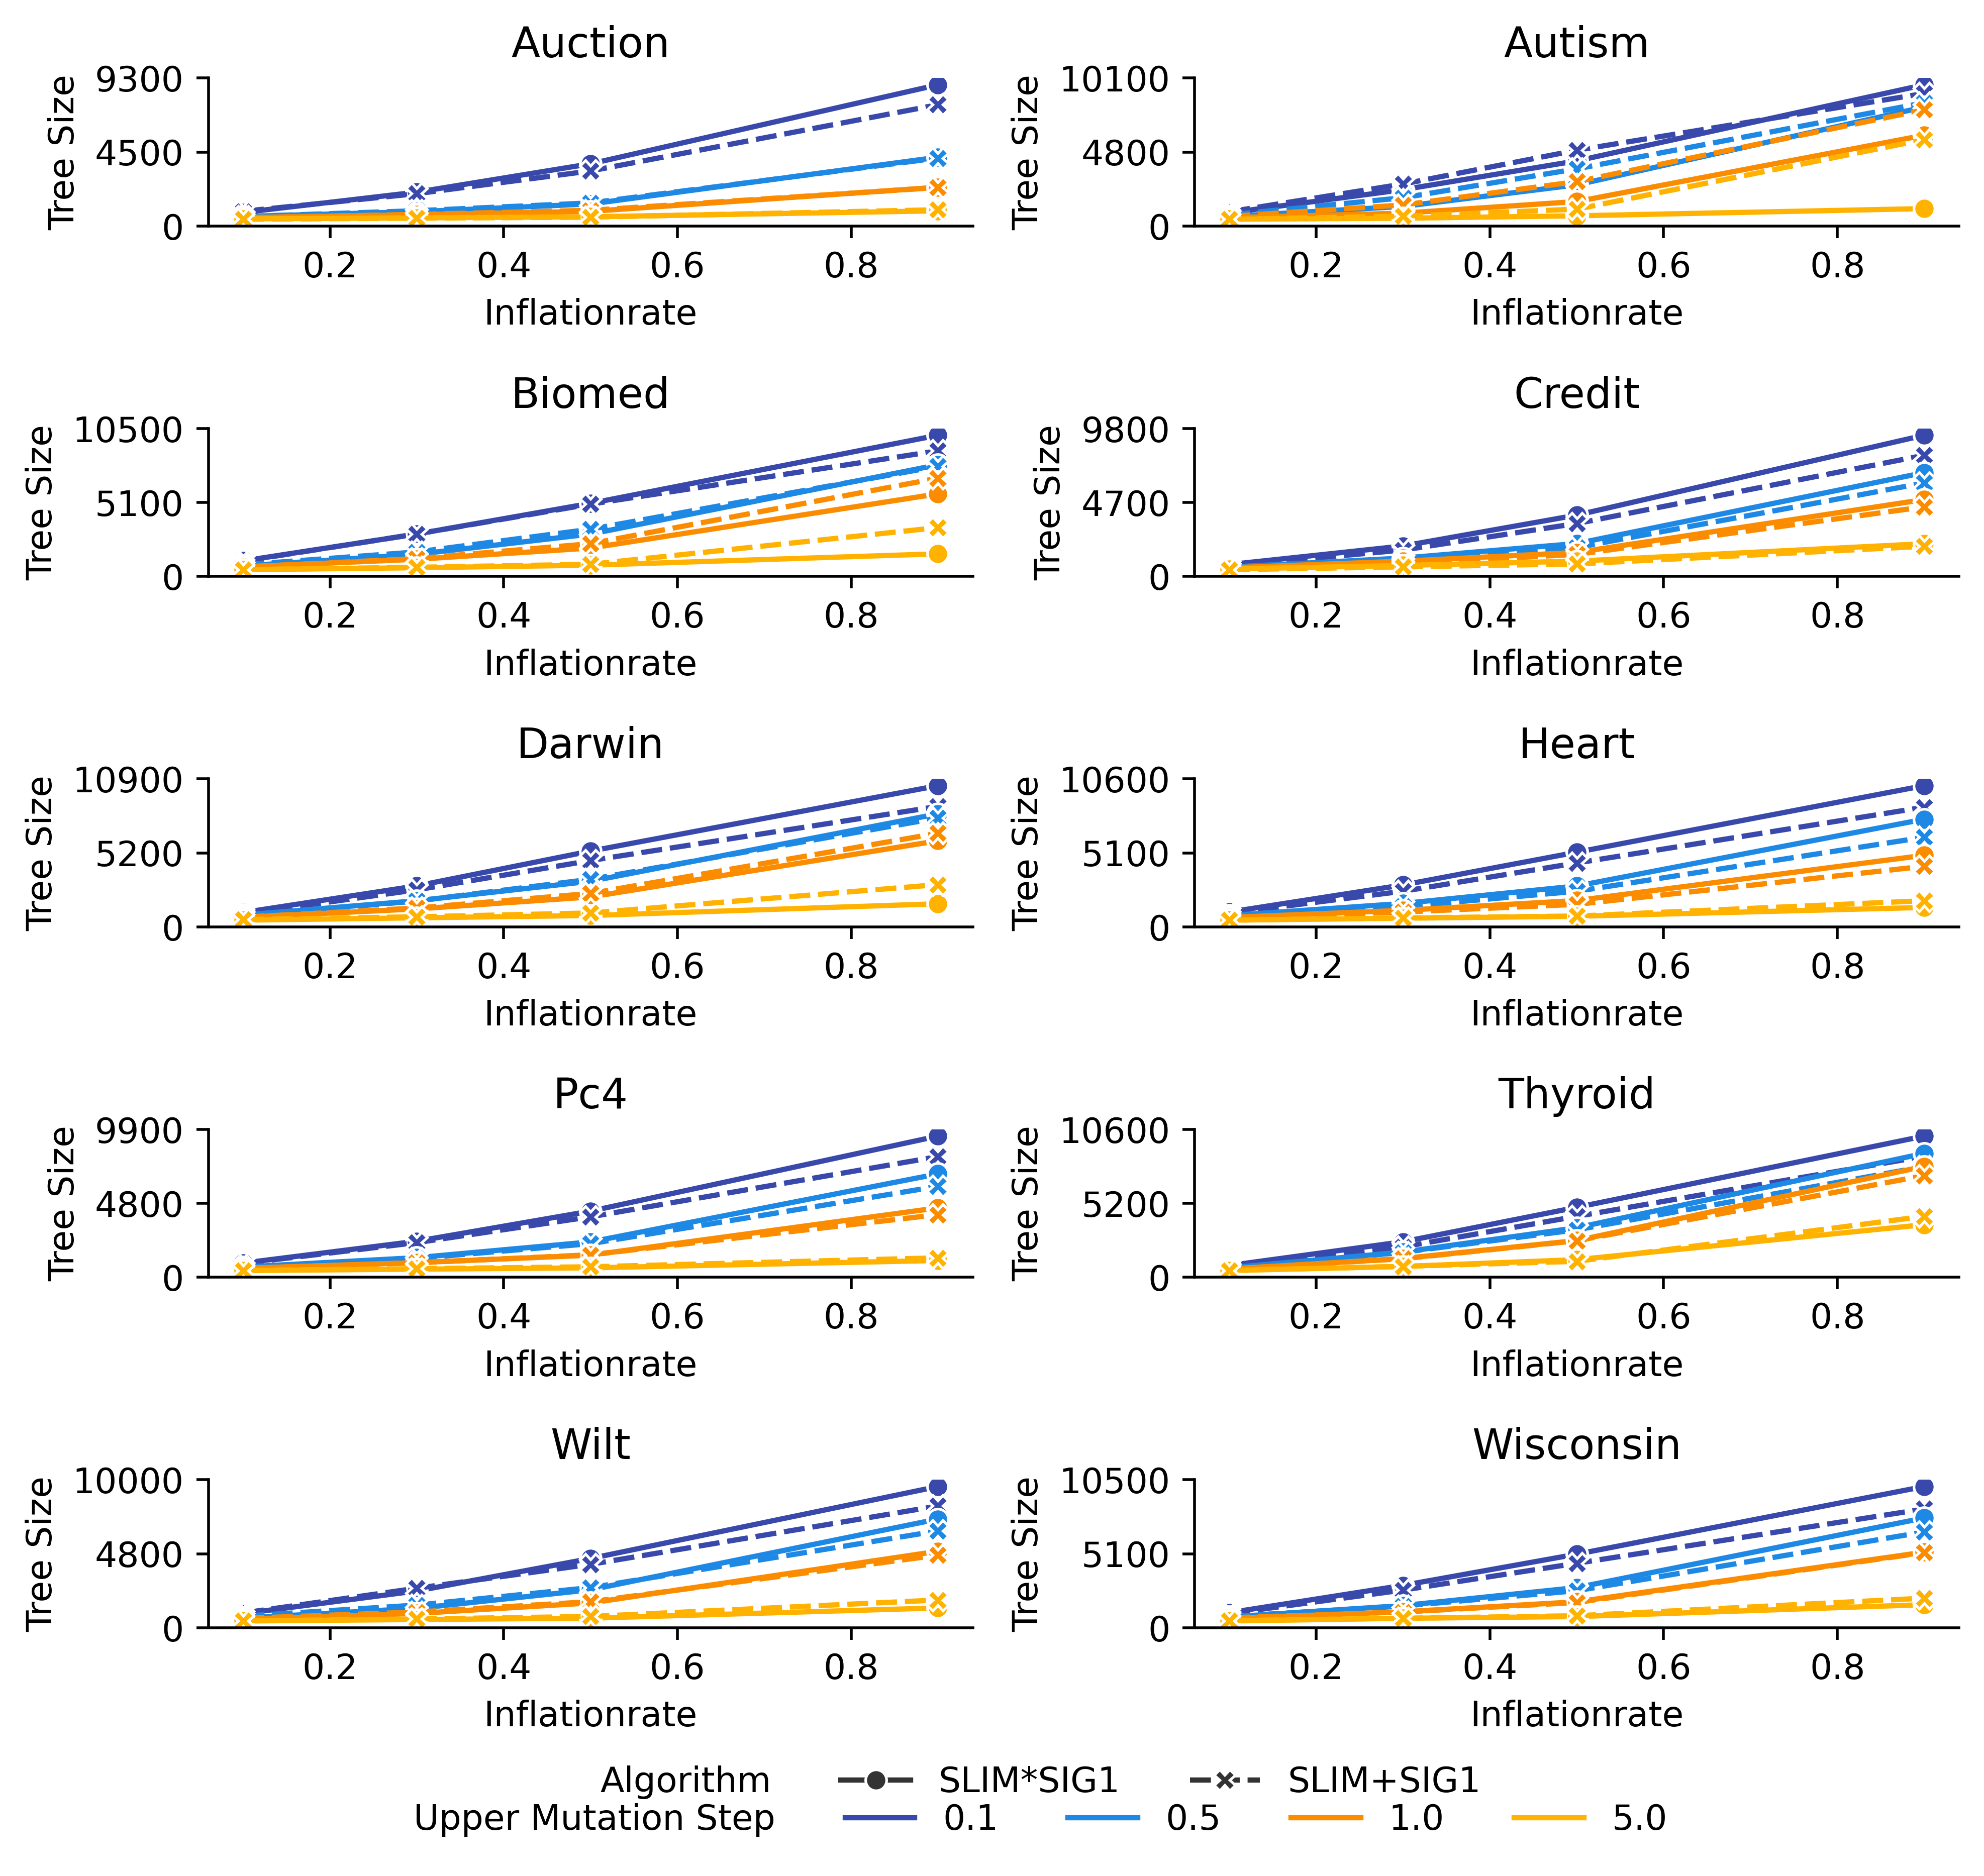
\includegraphics[width=\linewidth]{../Latex/Chapters/Figures/Results/RQ_Inflationrate_tree_size_by_p_inflate.png}
    \caption{Tree Size by Inflationrate}
    \label{fig:RQ_Inflationrate_tree_size_by_p_inflate}
    \end{figure}
    
\newpage

    \begin{figure}[H]
    \centering
    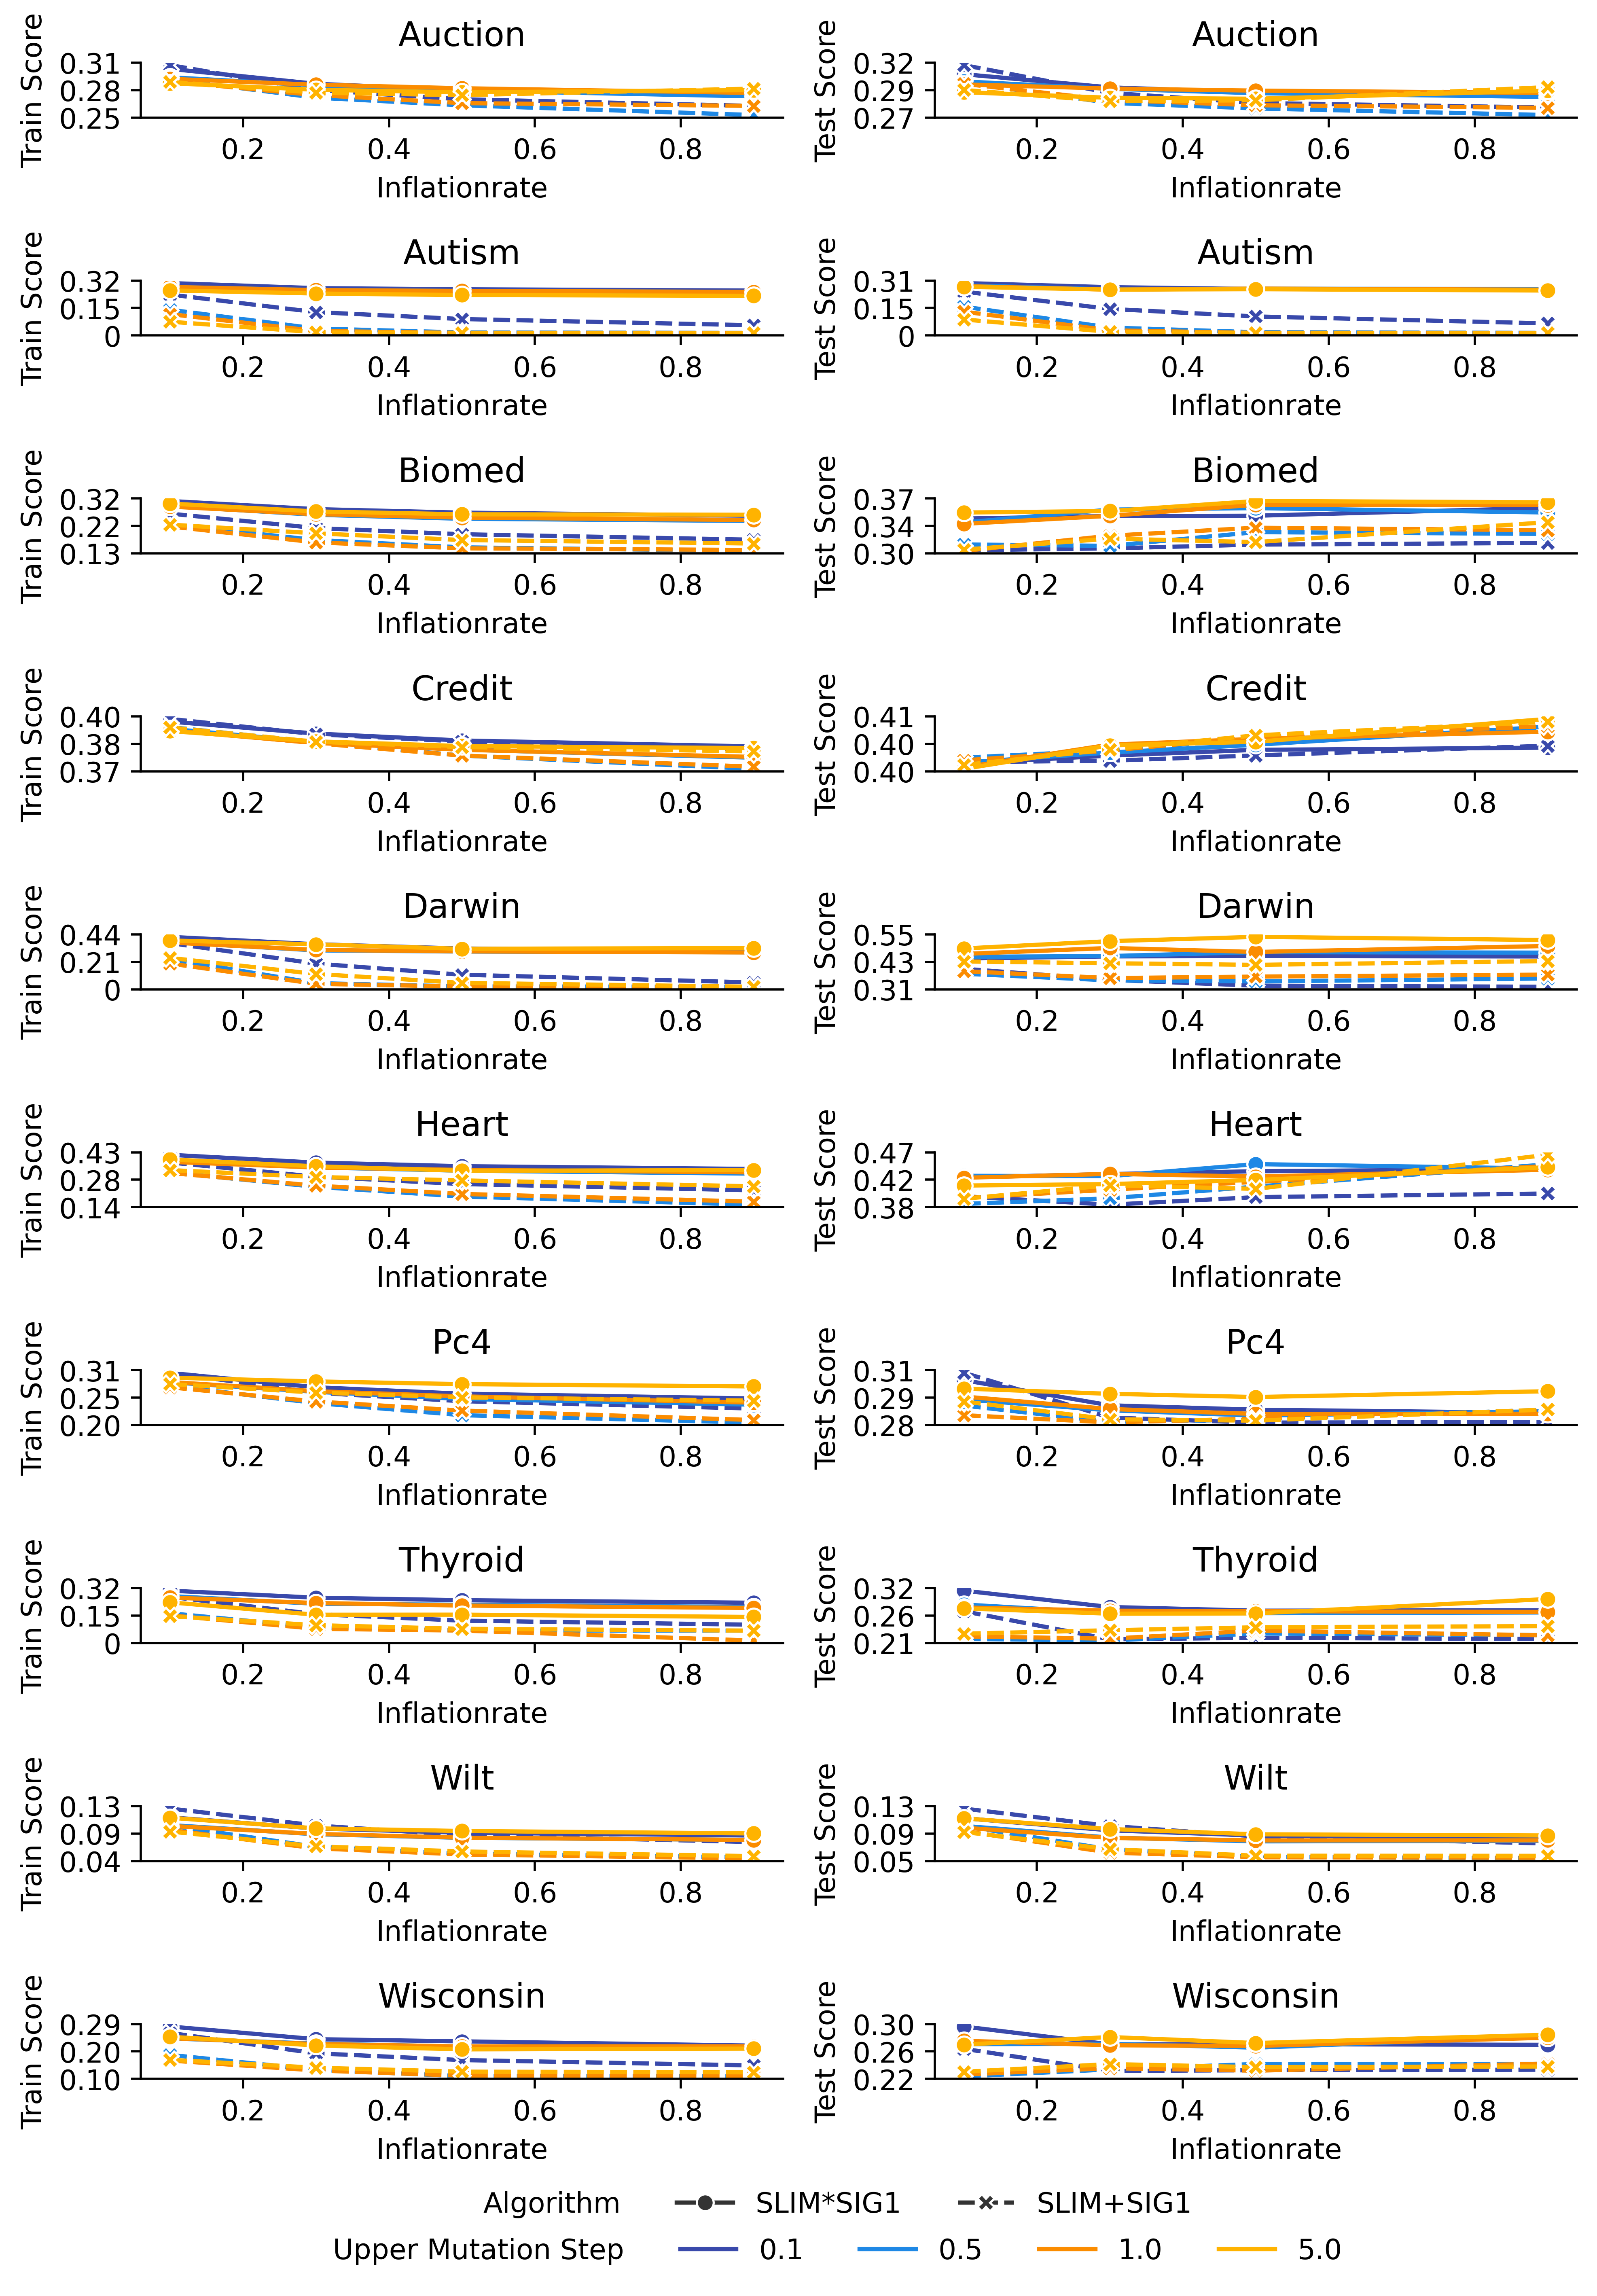
\includegraphics[width=\linewidth]{../Latex/Chapters/Figures/Results/RQ_Inflationrate_performance_by_p_inflate.png}
    \caption{Performance by Inflationrate}
    \label{fig:RQ_Inflationrate_performance_by_p_inflate}
    \end{figure}
    
\newpage

    \begin{figure}[H]
    \centering
    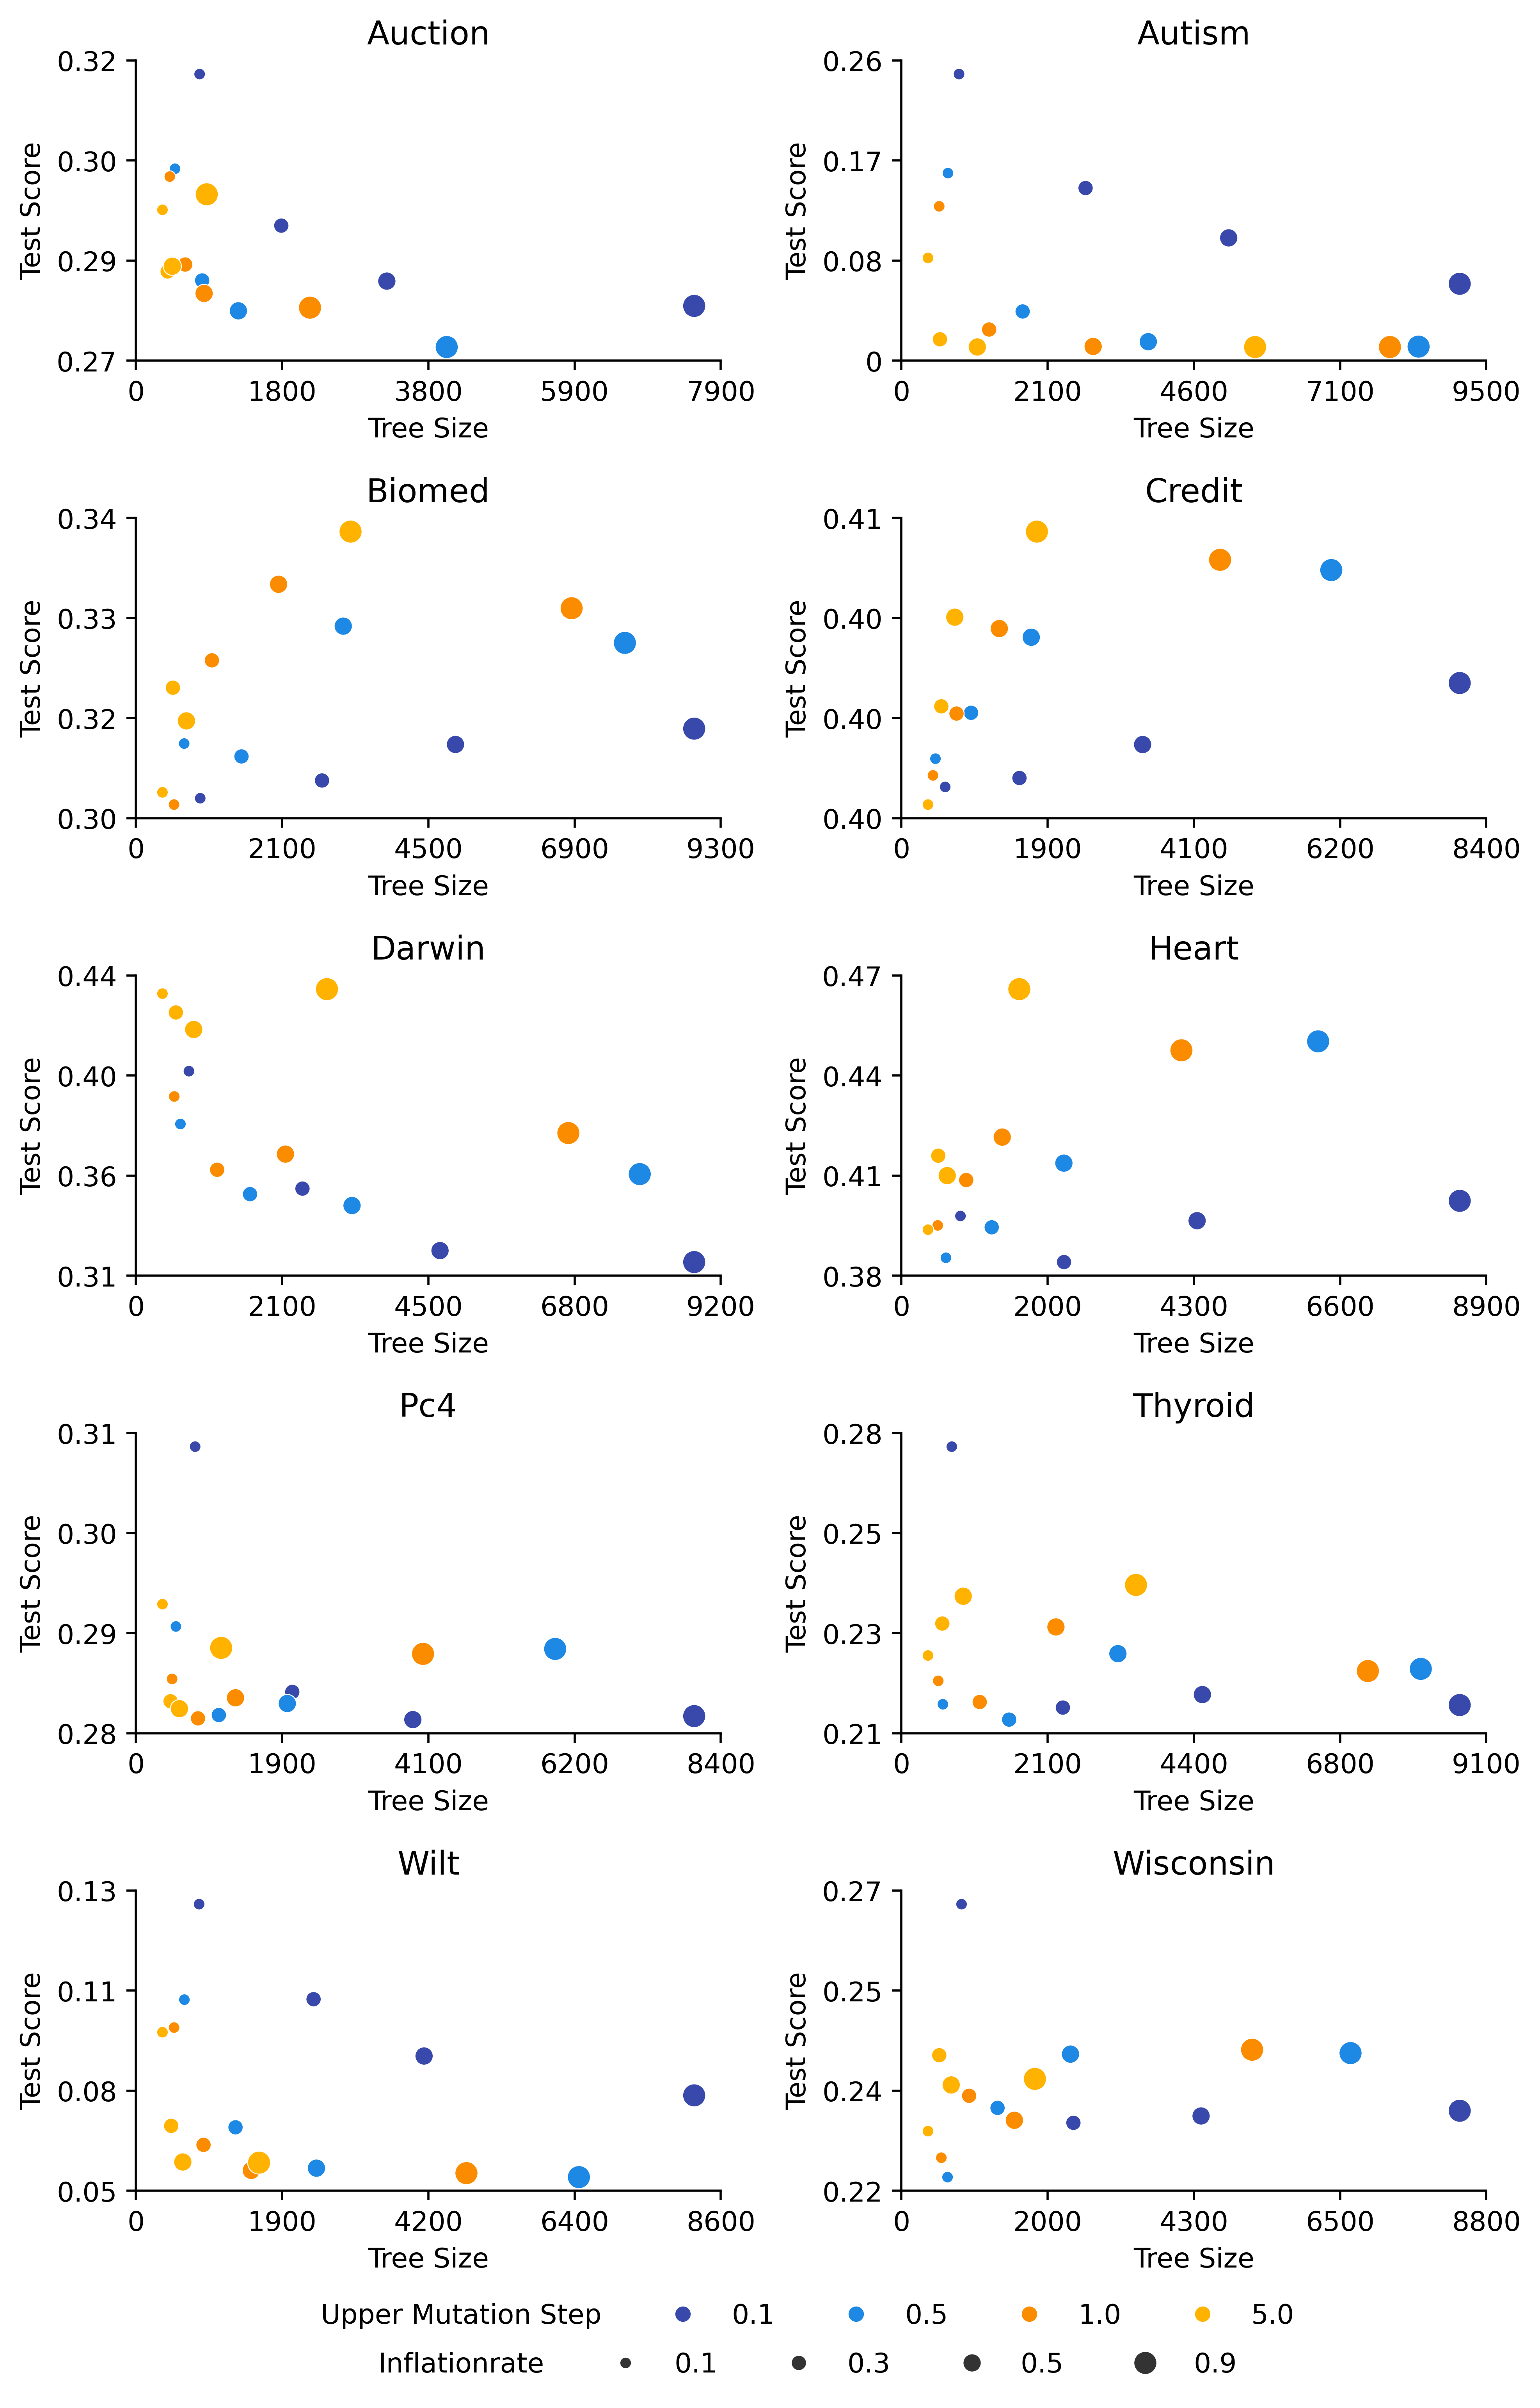
\includegraphics[width=\linewidth]{../Latex/Chapters/Figures/Results/RQ_Inflationrate_performance_complexity_tradeoff_plussig1.png}
    \caption{Performance-Complexity-Tradeoff SLIM+SIG1}
    \label{fig:RQ_Inflationrate_performance_complexity_tradeoff_plussig1}
    \end{figure}
    
\newpage

    \begin{figure}[H]
    \centering
    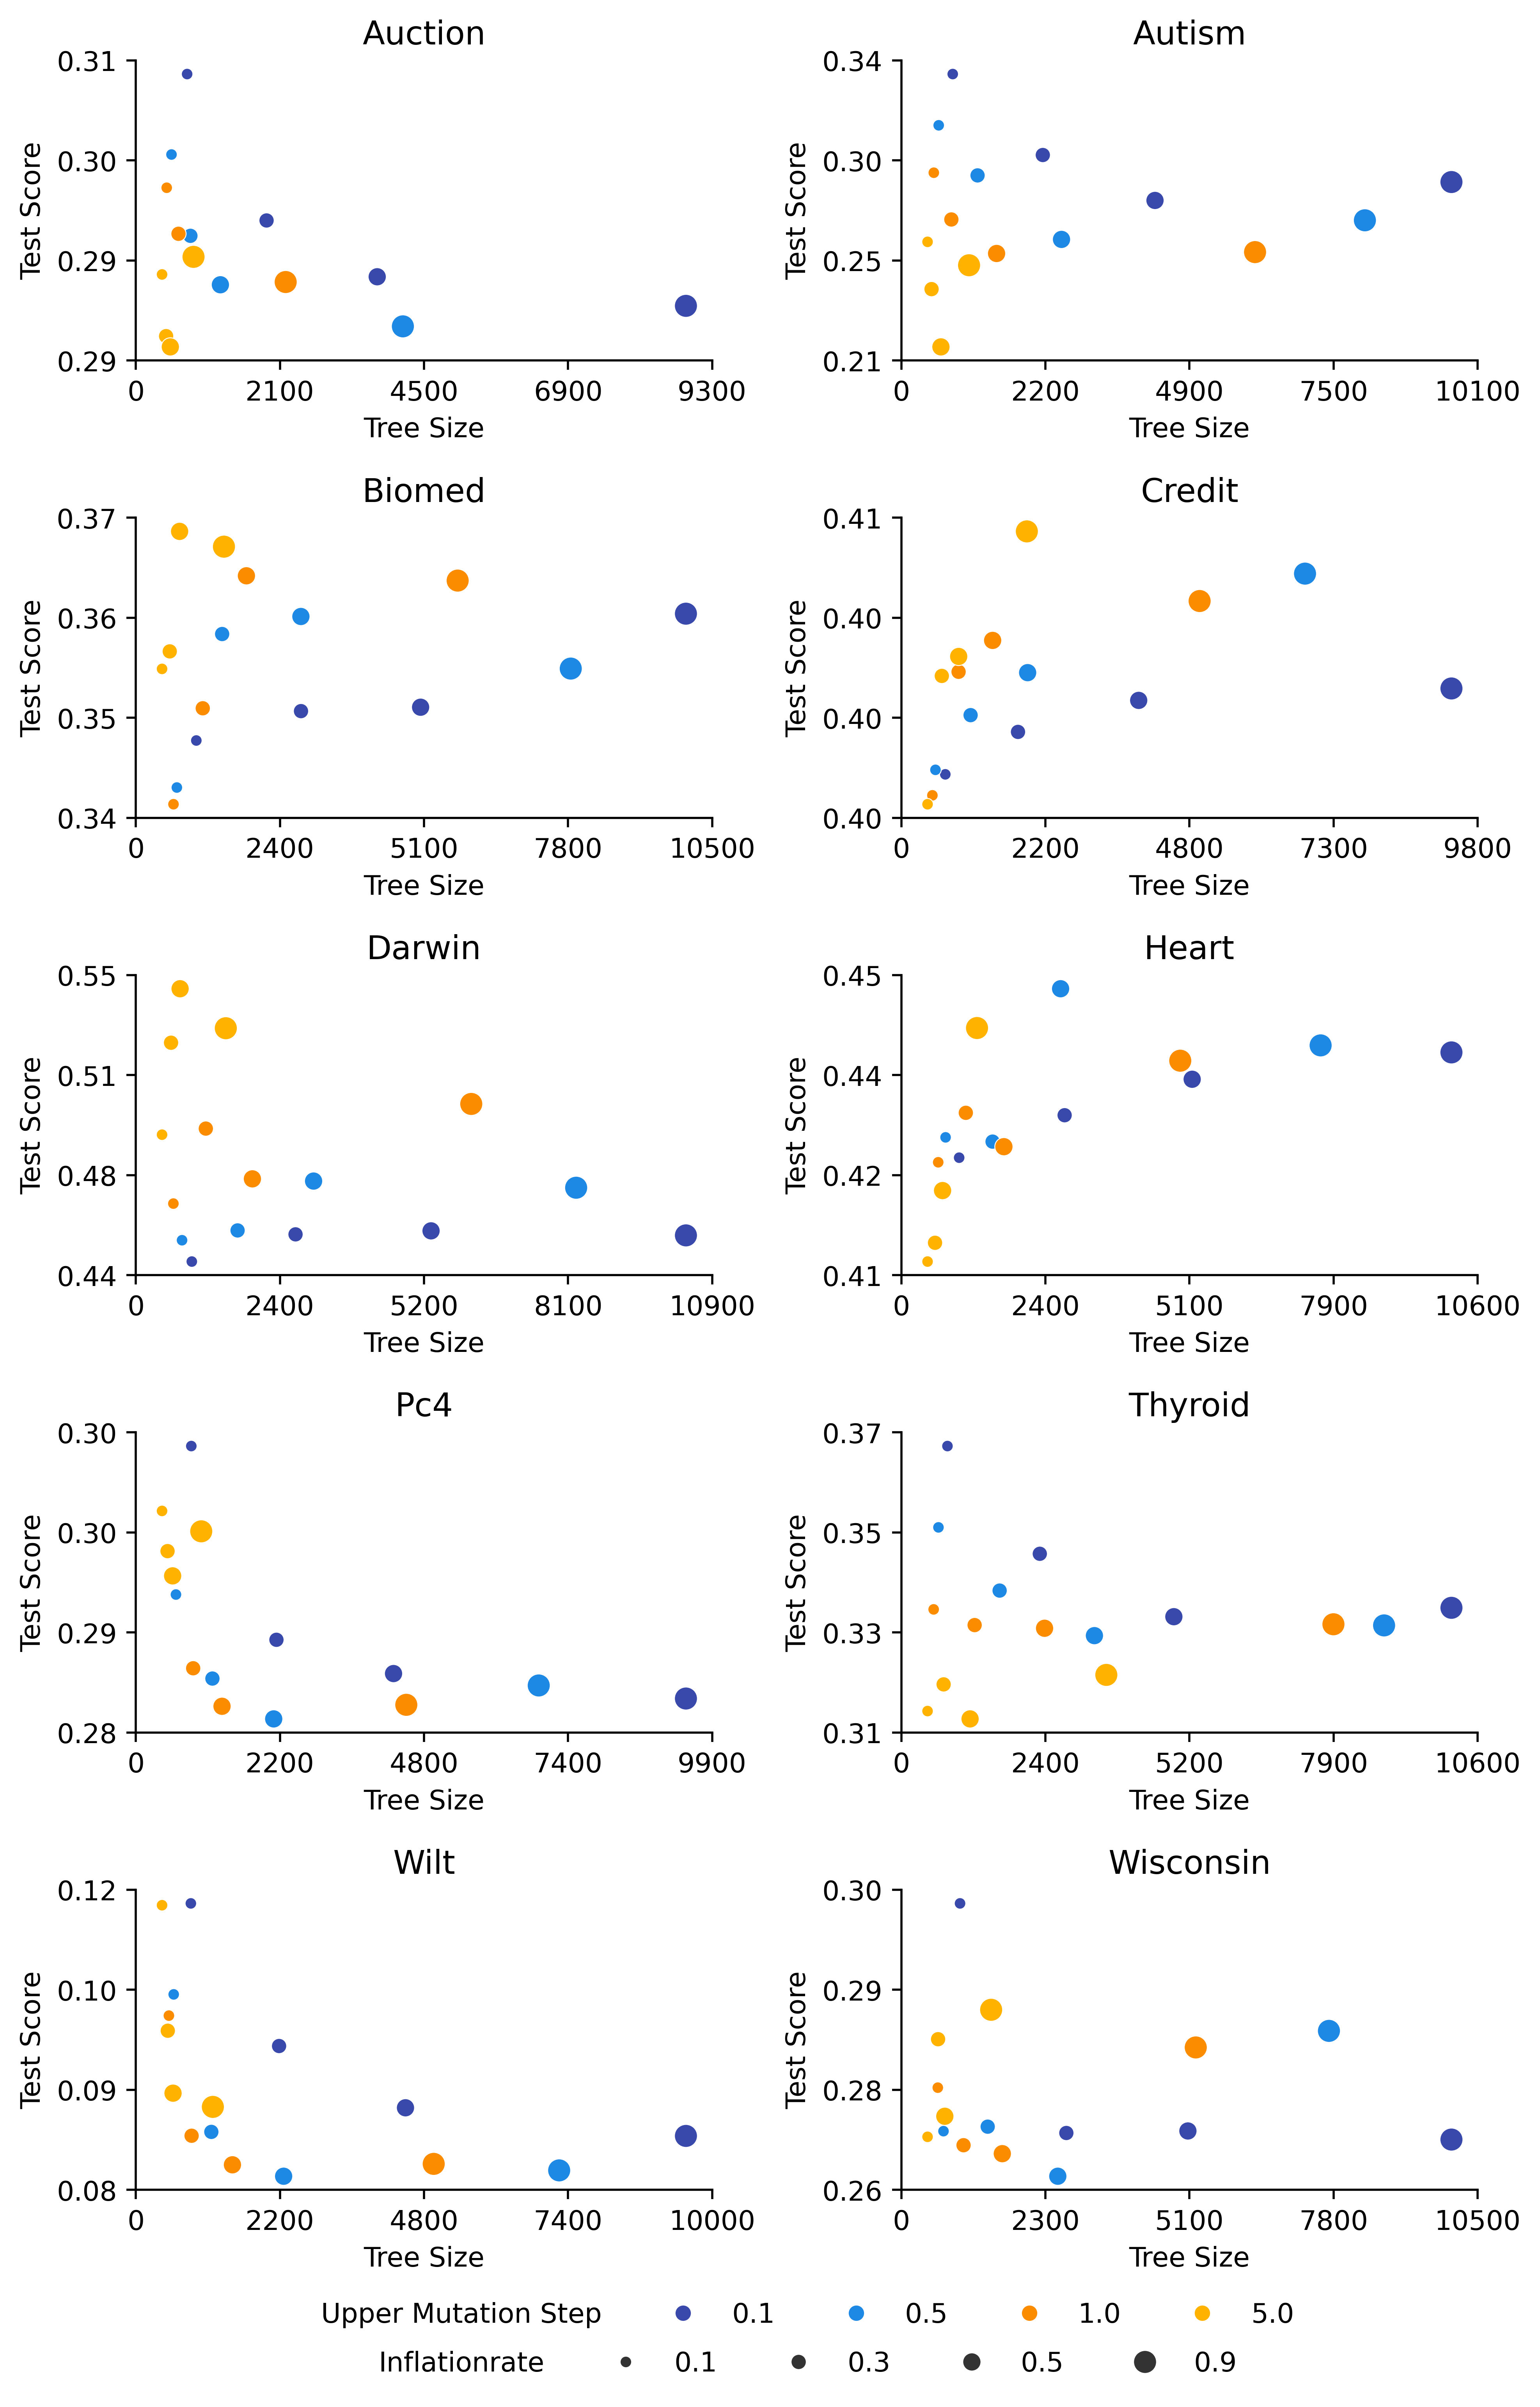
\includegraphics[width=\linewidth]{../Latex/Chapters/Figures/Results/RQ_Inflationrate_performance_complexity_tradeoff_mulsig1.png}
    \caption{Performance-Complexity-Tradeoff SLIM*SIG1}
    \label{fig:RQ_Inflationrate_performance_complexity_tradeoff_mulsig1}
    \end{figure}
    
\newpage

    \begin{table}[H]
        \centering
        \renewcommand{\arraystretch}{1.2}
        \caption{Tradeoff between Performance and Complexity}
        \label{tab:RQ_Inflationrate_tradeoff}
    \begin{tabular}{lccccccccccc}
\toprule
Dataset & Version & \multicolumn{2}{r}{Inflationrate} & \multicolumn{2}{r}{Upper MS} & \multicolumn{2}{r}{RMSE} & RMSE \% & \multicolumn{2}{r}{Tree Size} & Tree Size \% \\
 &  &  R &  T &  R &  T &  R &  T &  &  R &  T &  \\
\midrule
Auction & SLIM*SIG1 & 0.500000 & 0.500000 & 5.000000 & 5.000000 & 0.286600 & 0.286600 & +0.0\% & 232.500000 & 232.500000 & 0.0\% \\
Auction & SLIM+SIG1 & 0.900000 & 0.500000 & 0.500000 & 0.500000 & 0.273000 & 0.278500 & +2.0\% & 4066.500000 & 1136.500000 & -72.1\% \\
Autism & SLIM*SIG1 & 0.500000 & 0.500000 & 5.000000 & 5.000000 & 0.214900 & 0.214900 & +0.0\% & 344.000000 & 344.000000 & 0.0\% \\
Autism & SLIM+SIG1 & 0.900000 & 0.300000 & 5.000000 & 5.000000 & 0.000000 & 0.007000 & +inf\% & 5731.500000 & 319.000000 & -94.4\% \\
Biomed & SLIM*SIG1 & 0.100000 & 0.100000 & 1.000000 & 1.000000 & 0.339100 & 0.339100 & +0.0\% & 346.500000 & 346.500000 & 0.0\% \\
Biomed & SLIM+SIG1 & 0.100000 & 0.100000 & 1.000000 & 1.000000 & 0.303600 & 0.303600 & +0.0\% & 327.000000 & 327.000000 & 0.0\% \\
Credit & SLIM*SIG1 & 0.100000 & 0.100000 & 5.000000 & 5.000000 & 0.396000 & 0.396000 & +0.0\% & 158.500000 & 158.500000 & 0.0\% \\
Credit & SLIM+SIG1 & 0.100000 & 0.100000 & 5.000000 & 5.000000 & 0.396900 & 0.396900 & +0.0\% & 114.500000 & 114.500000 & 0.0\% \\
Darwin & SLIM*SIG1 & 0.100000 & 0.100000 & 0.100000 & 0.100000 & 0.445800 & 0.445800 & +0.0\% & 713.500000 & 713.500000 & 0.0\% \\
Darwin & SLIM+SIG1 & 0.900000 & 0.300000 & 0.100000 & 0.500000 & 0.319500 & 0.348100 & +9.0\% & 8771.000000 & 1587.000000 & -81.9\% \\
Heart & SLIM*SIG1 & 0.100000 & 0.100000 & 5.000000 & 5.000000 & 0.411600 & 0.411600 & +0.0\% & 102.500000 & 102.500000 & 0.0\% \\
Heart & SLIM+SIG1 & 0.300000 & 0.100000 & 0.100000 & 0.500000 & 0.380700 & 0.382000 & +0.3\% & 2255.000000 & 386.500000 & -82.9\% \\
Pc4 & SLIM*SIG1 & 0.500000 & 0.500000 & 0.500000 & 1.000000 & 0.281500 & 0.282500 & +0.4\% & 2080.500000 & 1155.000000 & -44.5\% \\
Pc4 & SLIM+SIG1 & 0.500000 & 0.500000 & 0.100000 & 5.000000 & 0.277200 & 0.278400 & +0.4\% & 3831.000000 & 345.000000 & -91.0\% \\
Thyroid & SLIM*SIG1 & 0.500000 & 0.100000 & 5.000000 & 5.000000 & 0.311100 & 0.312800 & +0.5\% & 982.000000 & 174.000000 & -82.3\% \\
Thyroid & SLIM+SIG1 & 0.900000 & 0.100000 & 0.100000 & 1.000000 & 0.201100 & 0.207800 & +3.4\% & 8634.500000 & 297.500000 & -96.6\% \\
Wilt & SLIM*SIG1 & 0.500000 & 0.500000 & 0.500000 & 1.000000 & 0.080200 & 0.081700 & +1.8\% & 2294.500000 & 1368.000000 & -40.4\% \\
Wilt & SLIM+SIG1 & 0.900000 & 0.500000 & 0.500000 & 5.000000 & 0.054500 & 0.058700 & +7.6\% & 6447.500000 & 413.000000 & -93.6\% \\
Wisconsin & SLIM*SIG1 & 0.500000 & 0.300000 & 0.500000 & 1.000000 & 0.265500 & 0.269100 & +1.4\% & 2582.000000 & 802.000000 & -68.9\% \\
Wisconsin & SLIM+SIG1 & 0.100000 & 0.100000 & 0.500000 & 0.500000 & 0.222100 & 0.222100 & +0.0\% & 452.000000 & 452.000000 & 0.0\% \\
\bottomrule
\end{tabular}

        
    \end{table}
    

    \begin{table}[H]
        \centering
        \renewcommand{\arraystretch}{1.2}
        \caption{Tradeoff between Performance and Complexity}
        \label{tab:RQ_Inflationrate_tradeoff}
    \begin{tabular}{lccccccccccc}
\toprule
Dataset & Version & \multicolumn{2}{r}{Inflationrate} & \multicolumn{2}{r}{Upper MS} & \multicolumn{2}{r}{RMSE} & RMSE \% & \multicolumn{2}{r}{Tree Size} & Tree Size \% \\
 &  &  R &  T &  R &  T &  R &  T &  &  R &  T &  \\
\midrule
Auction & SLIM*SIG1 & 0.500000 & 0.500000 & 5.000000 & 5.000000 & 0.286600 & 0.286600 & +0.0\% & 232.500000 & 232.500000 & 0.0\% \\
Auction & SLIM+SIG1 & 0.900000 & 0.500000 & 0.500000 & 0.500000 & 0.273000 & 0.278500 & +2.0\% & 4066.500000 & 1136.500000 & -72.1\% \\
Autism & SLIM*SIG1 & 0.500000 & 0.500000 & 5.000000 & 5.000000 & 0.214900 & 0.214900 & +0.0\% & 344.000000 & 344.000000 & 0.0\% \\
Autism & SLIM+SIG1 & 0.900000 & 0.300000 & 5.000000 & 5.000000 & 0.000000 & 0.007000 & +inf\% & 5731.500000 & 319.000000 & -94.4\% \\
Biomed & SLIM*SIG1 & 0.100000 & 0.100000 & 1.000000 & 1.000000 & 0.339100 & 0.339100 & +0.0\% & 346.500000 & 346.500000 & 0.0\% \\
Biomed & SLIM+SIG1 & 0.100000 & 0.100000 & 1.000000 & 1.000000 & 0.303600 & 0.303600 & +0.0\% & 327.000000 & 327.000000 & 0.0\% \\
Credit & SLIM*SIG1 & 0.100000 & 0.100000 & 5.000000 & 5.000000 & 0.396000 & 0.396000 & +0.0\% & 158.500000 & 158.500000 & 0.0\% \\
Credit & SLIM+SIG1 & 0.100000 & 0.100000 & 5.000000 & 5.000000 & 0.396900 & 0.396900 & +0.0\% & 114.500000 & 114.500000 & 0.0\% \\
Darwin & SLIM*SIG1 & 0.100000 & 0.100000 & 0.100000 & 0.100000 & 0.445800 & 0.445800 & +0.0\% & 713.500000 & 713.500000 & 0.0\% \\
Darwin & SLIM+SIG1 & 0.900000 & 0.300000 & 0.100000 & 0.500000 & 0.319500 & 0.348100 & +9.0\% & 8771.000000 & 1587.000000 & -81.9\% \\
Heart & SLIM*SIG1 & 0.100000 & 0.100000 & 5.000000 & 5.000000 & 0.411600 & 0.411600 & +0.0\% & 102.500000 & 102.500000 & 0.0\% \\
Heart & SLIM+SIG1 & 0.300000 & 0.100000 & 0.100000 & 0.500000 & 0.380700 & 0.382000 & +0.3\% & 2255.000000 & 386.500000 & -82.9\% \\
Pc4 & SLIM*SIG1 & 0.500000 & 0.500000 & 0.500000 & 1.000000 & 0.281500 & 0.282500 & +0.4\% & 2080.500000 & 1155.000000 & -44.5\% \\
Pc4 & SLIM+SIG1 & 0.500000 & 0.500000 & 0.100000 & 5.000000 & 0.277200 & 0.278400 & +0.4\% & 3831.000000 & 345.000000 & -91.0\% \\
Thyroid & SLIM*SIG1 & 0.500000 & 0.100000 & 5.000000 & 5.000000 & 0.311100 & 0.312800 & +0.5\% & 982.000000 & 174.000000 & -82.3\% \\
Thyroid & SLIM+SIG1 & 0.900000 & 0.100000 & 0.100000 & 1.000000 & 0.201100 & 0.207800 & +3.4\% & 8634.500000 & 297.500000 & -96.6\% \\
Wilt & SLIM*SIG1 & 0.500000 & 0.500000 & 0.500000 & 1.000000 & 0.080200 & 0.081700 & +1.8\% & 2294.500000 & 1368.000000 & -40.4\% \\
Wilt & SLIM+SIG1 & 0.900000 & 0.500000 & 0.500000 & 5.000000 & 0.054500 & 0.058700 & +7.6\% & 6447.500000 & 413.000000 & -93.6\% \\
Wisconsin & SLIM*SIG1 & 0.500000 & 0.300000 & 0.500000 & 1.000000 & 0.265500 & 0.269100 & +1.4\% & 2582.000000 & 802.000000 & -68.9\% \\
Wisconsin & SLIM+SIG1 & 0.100000 & 0.100000 & 0.500000 & 0.500000 & 0.222100 & 0.222100 & +0.0\% & 452.000000 & 452.000000 & 0.0\% \\
\bottomrule
\end{tabular}

        
    \end{table}
    

\subsection{Experiment 3: Comparison of SLIM-GSGP, GSGP and stdGP}
\label{app:exp3}

    \begin{figure}[H]
    \centering
    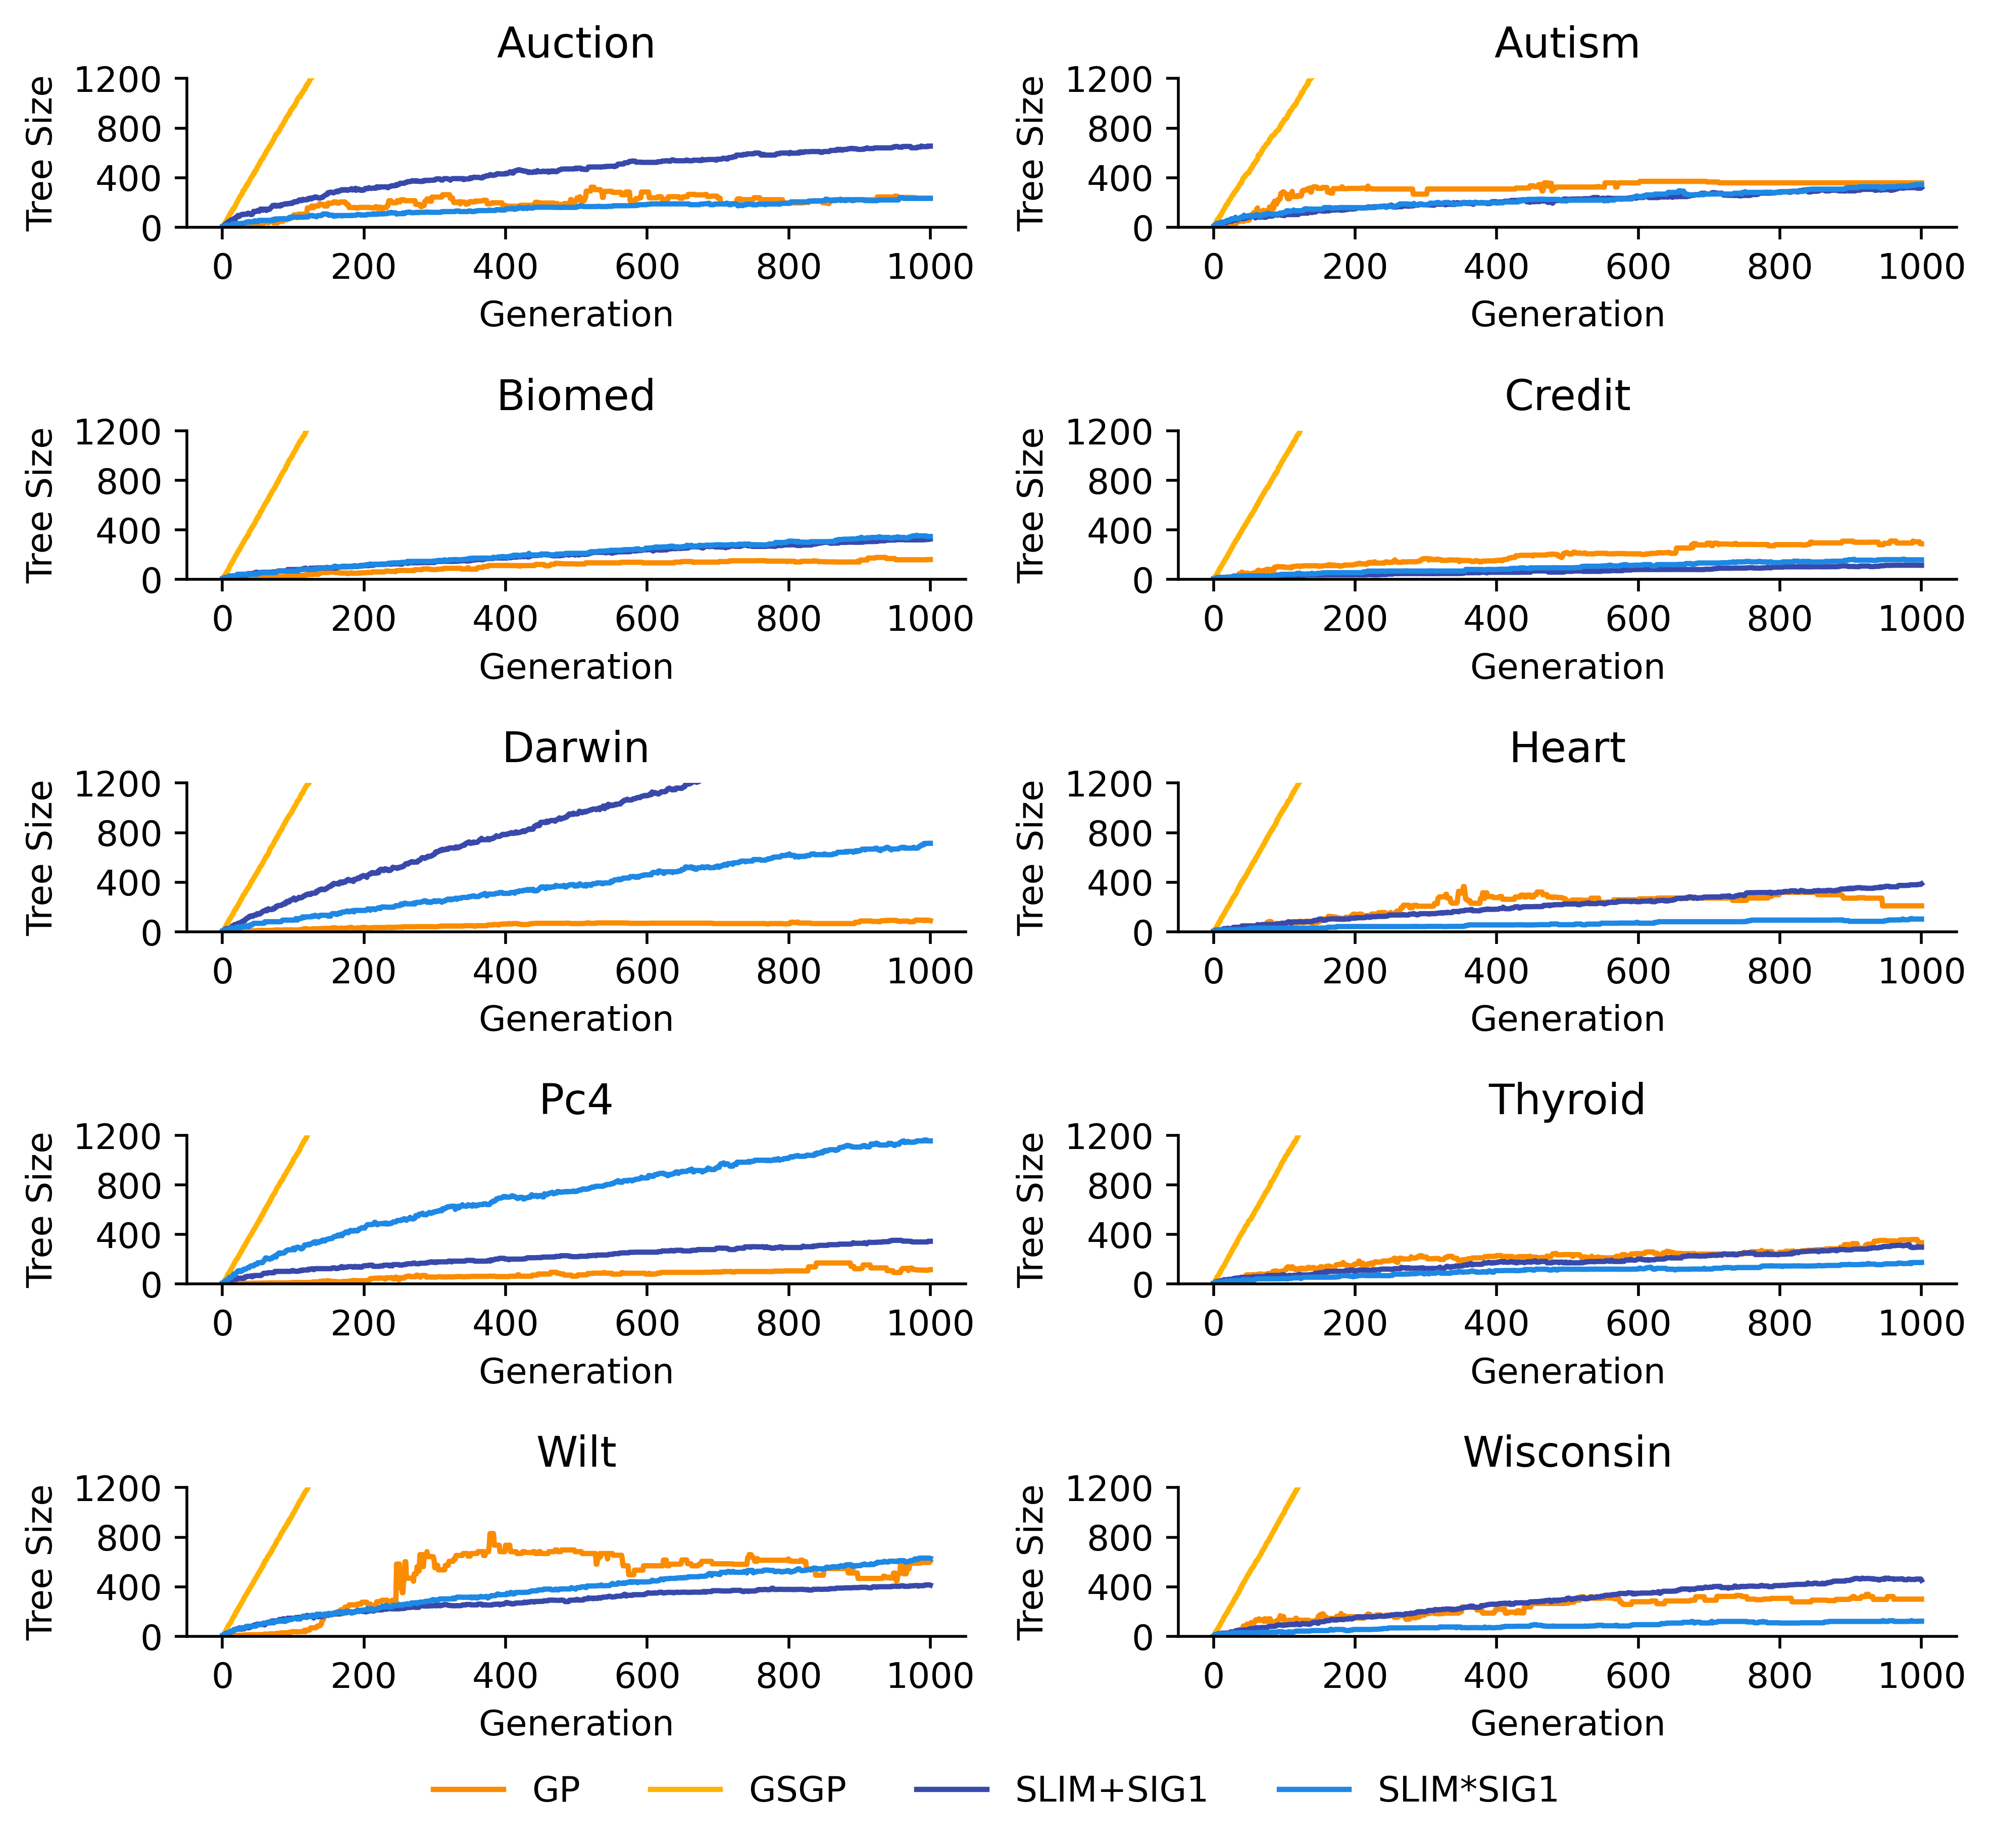
\includegraphics[width=\linewidth]{../Latex/Chapters/Figures/Results/RQ_Comparison_tree_size_evolution.png}
    \caption{Tree Size Evolution by Algorithm}
    \label{fig:RQ_Comparison_tree_size_evolution}
    \end{figure}
    
\newpage

    \begin{figure}[H]
    \centering
    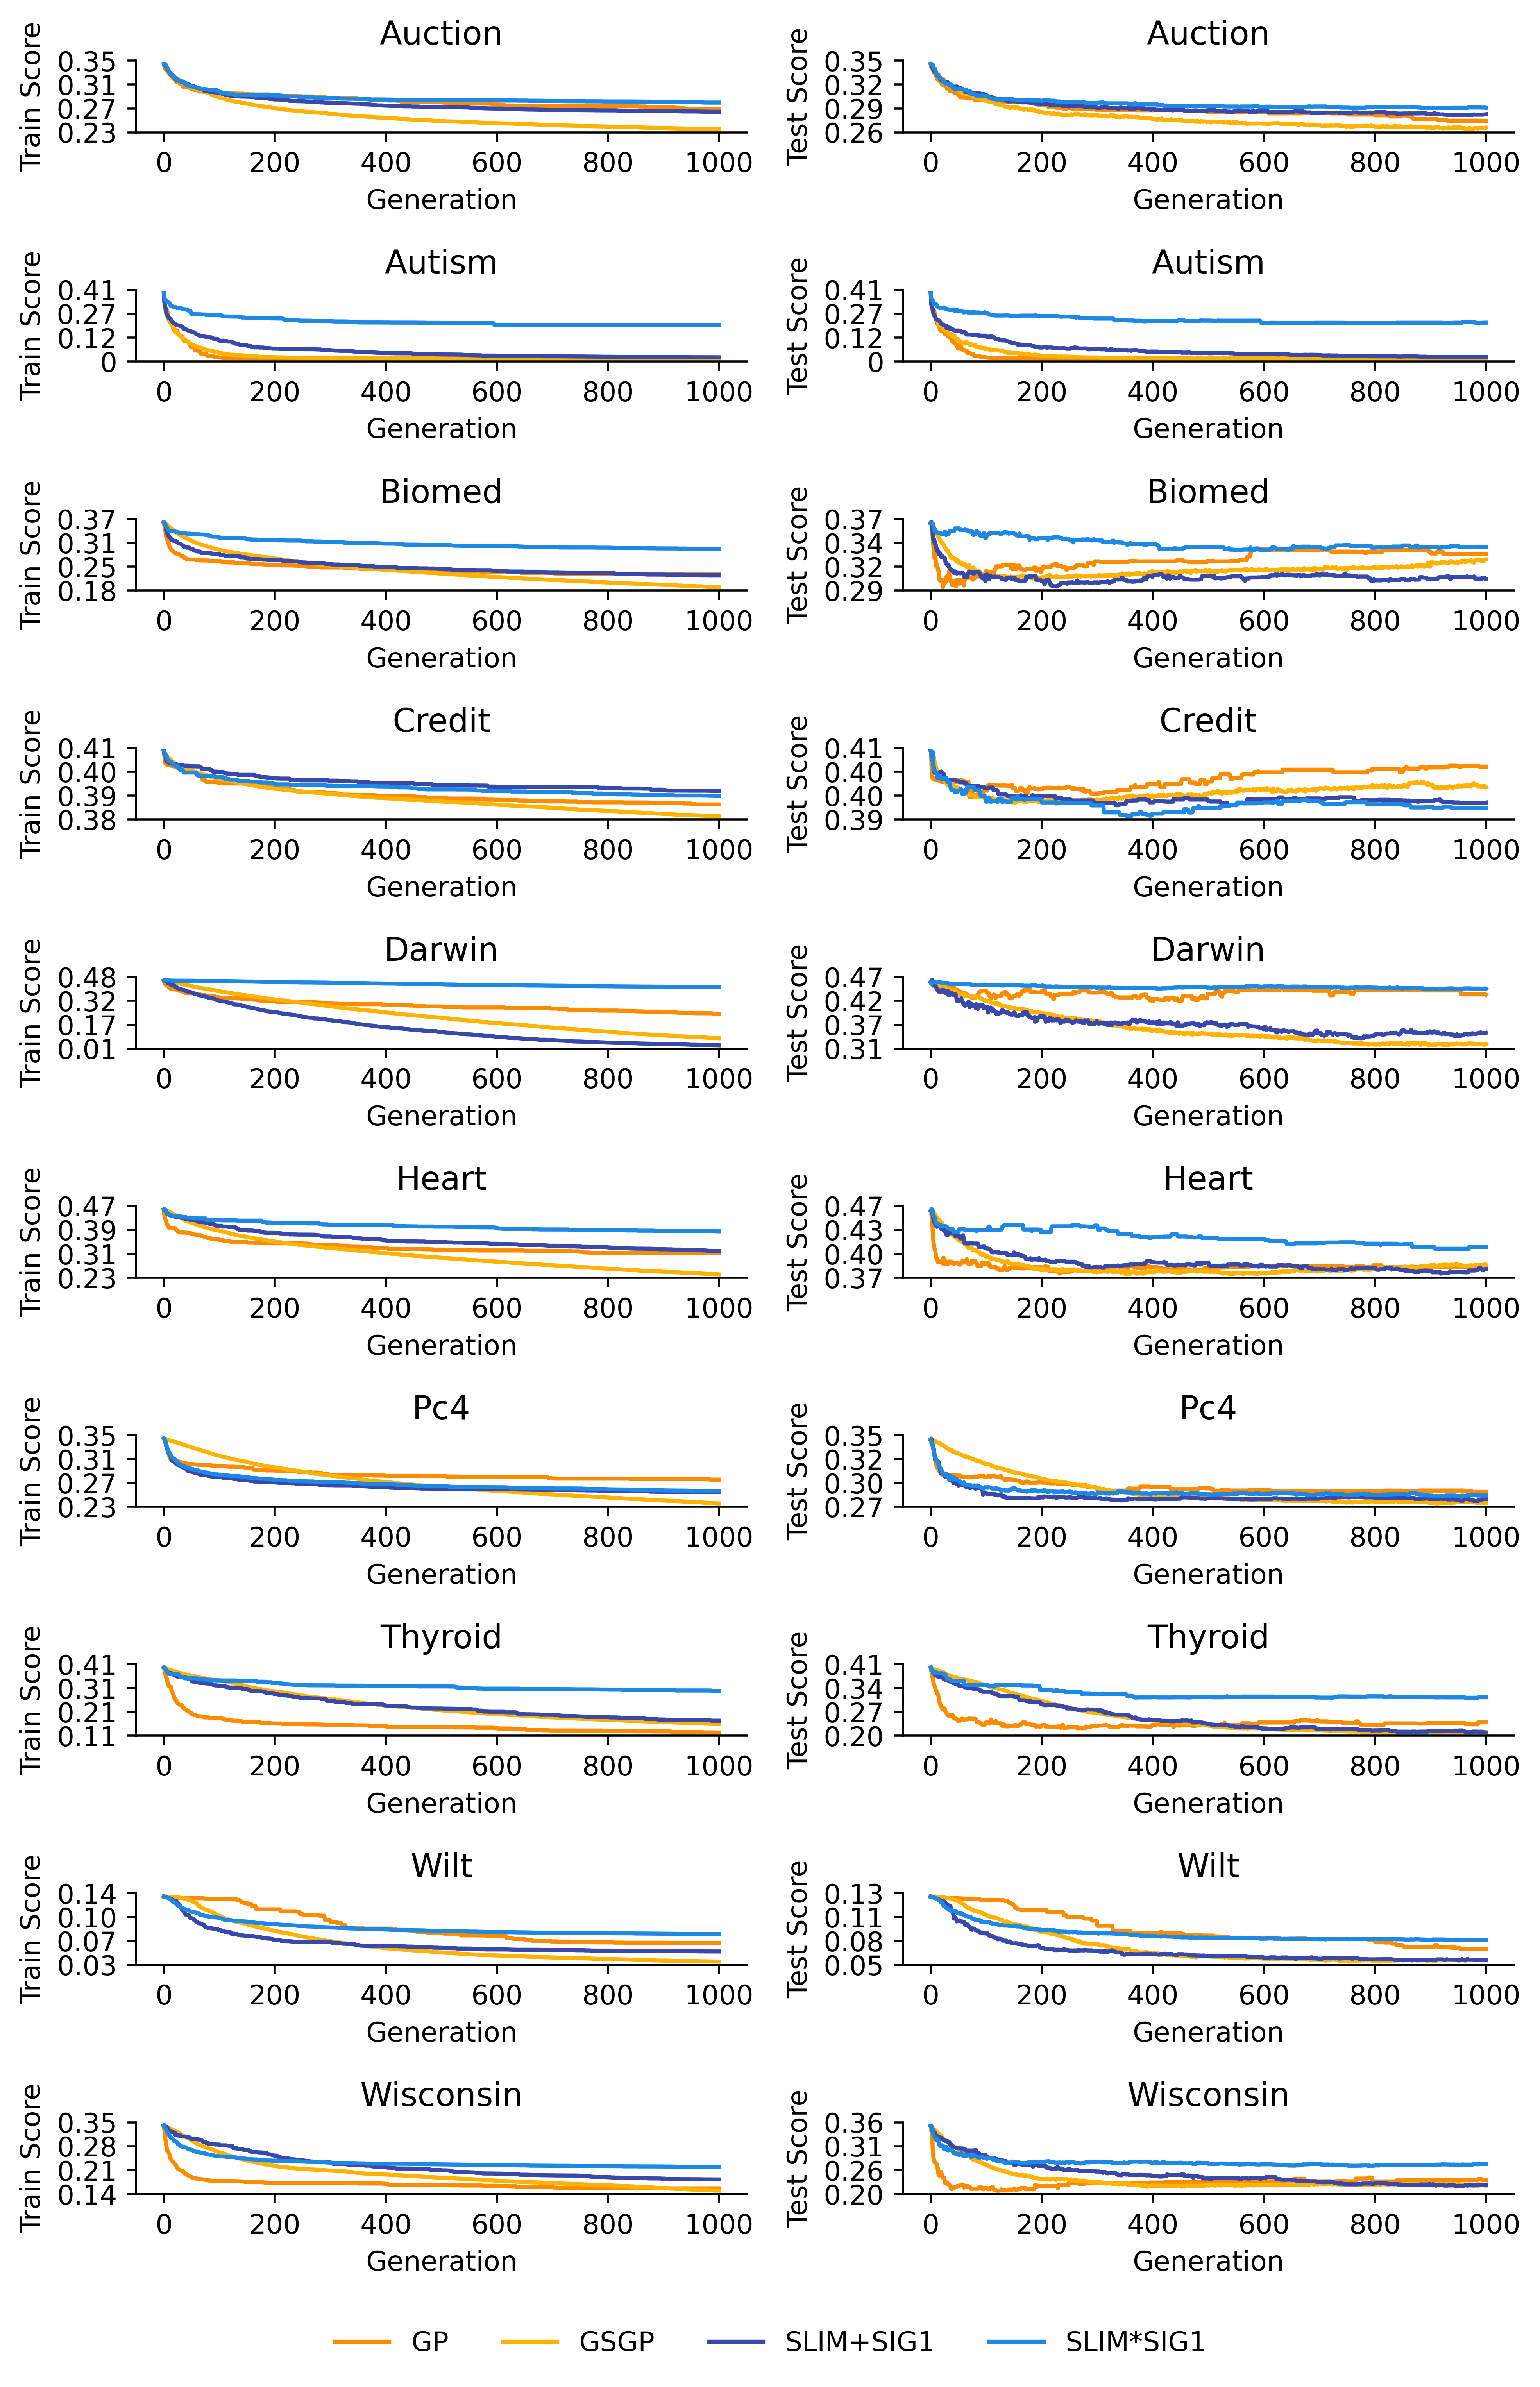
\includegraphics[width=\linewidth]{../Latex/Chapters/Figures/Results/RQ_Comparison_performance_evolution.png}
    \caption{Performance Evolution by Algorithm}
    \label{fig:RQ_Comparison_performance_evolution}
    \end{figure}
    
\newpage

    \begin{figure}[H]
    \centering
    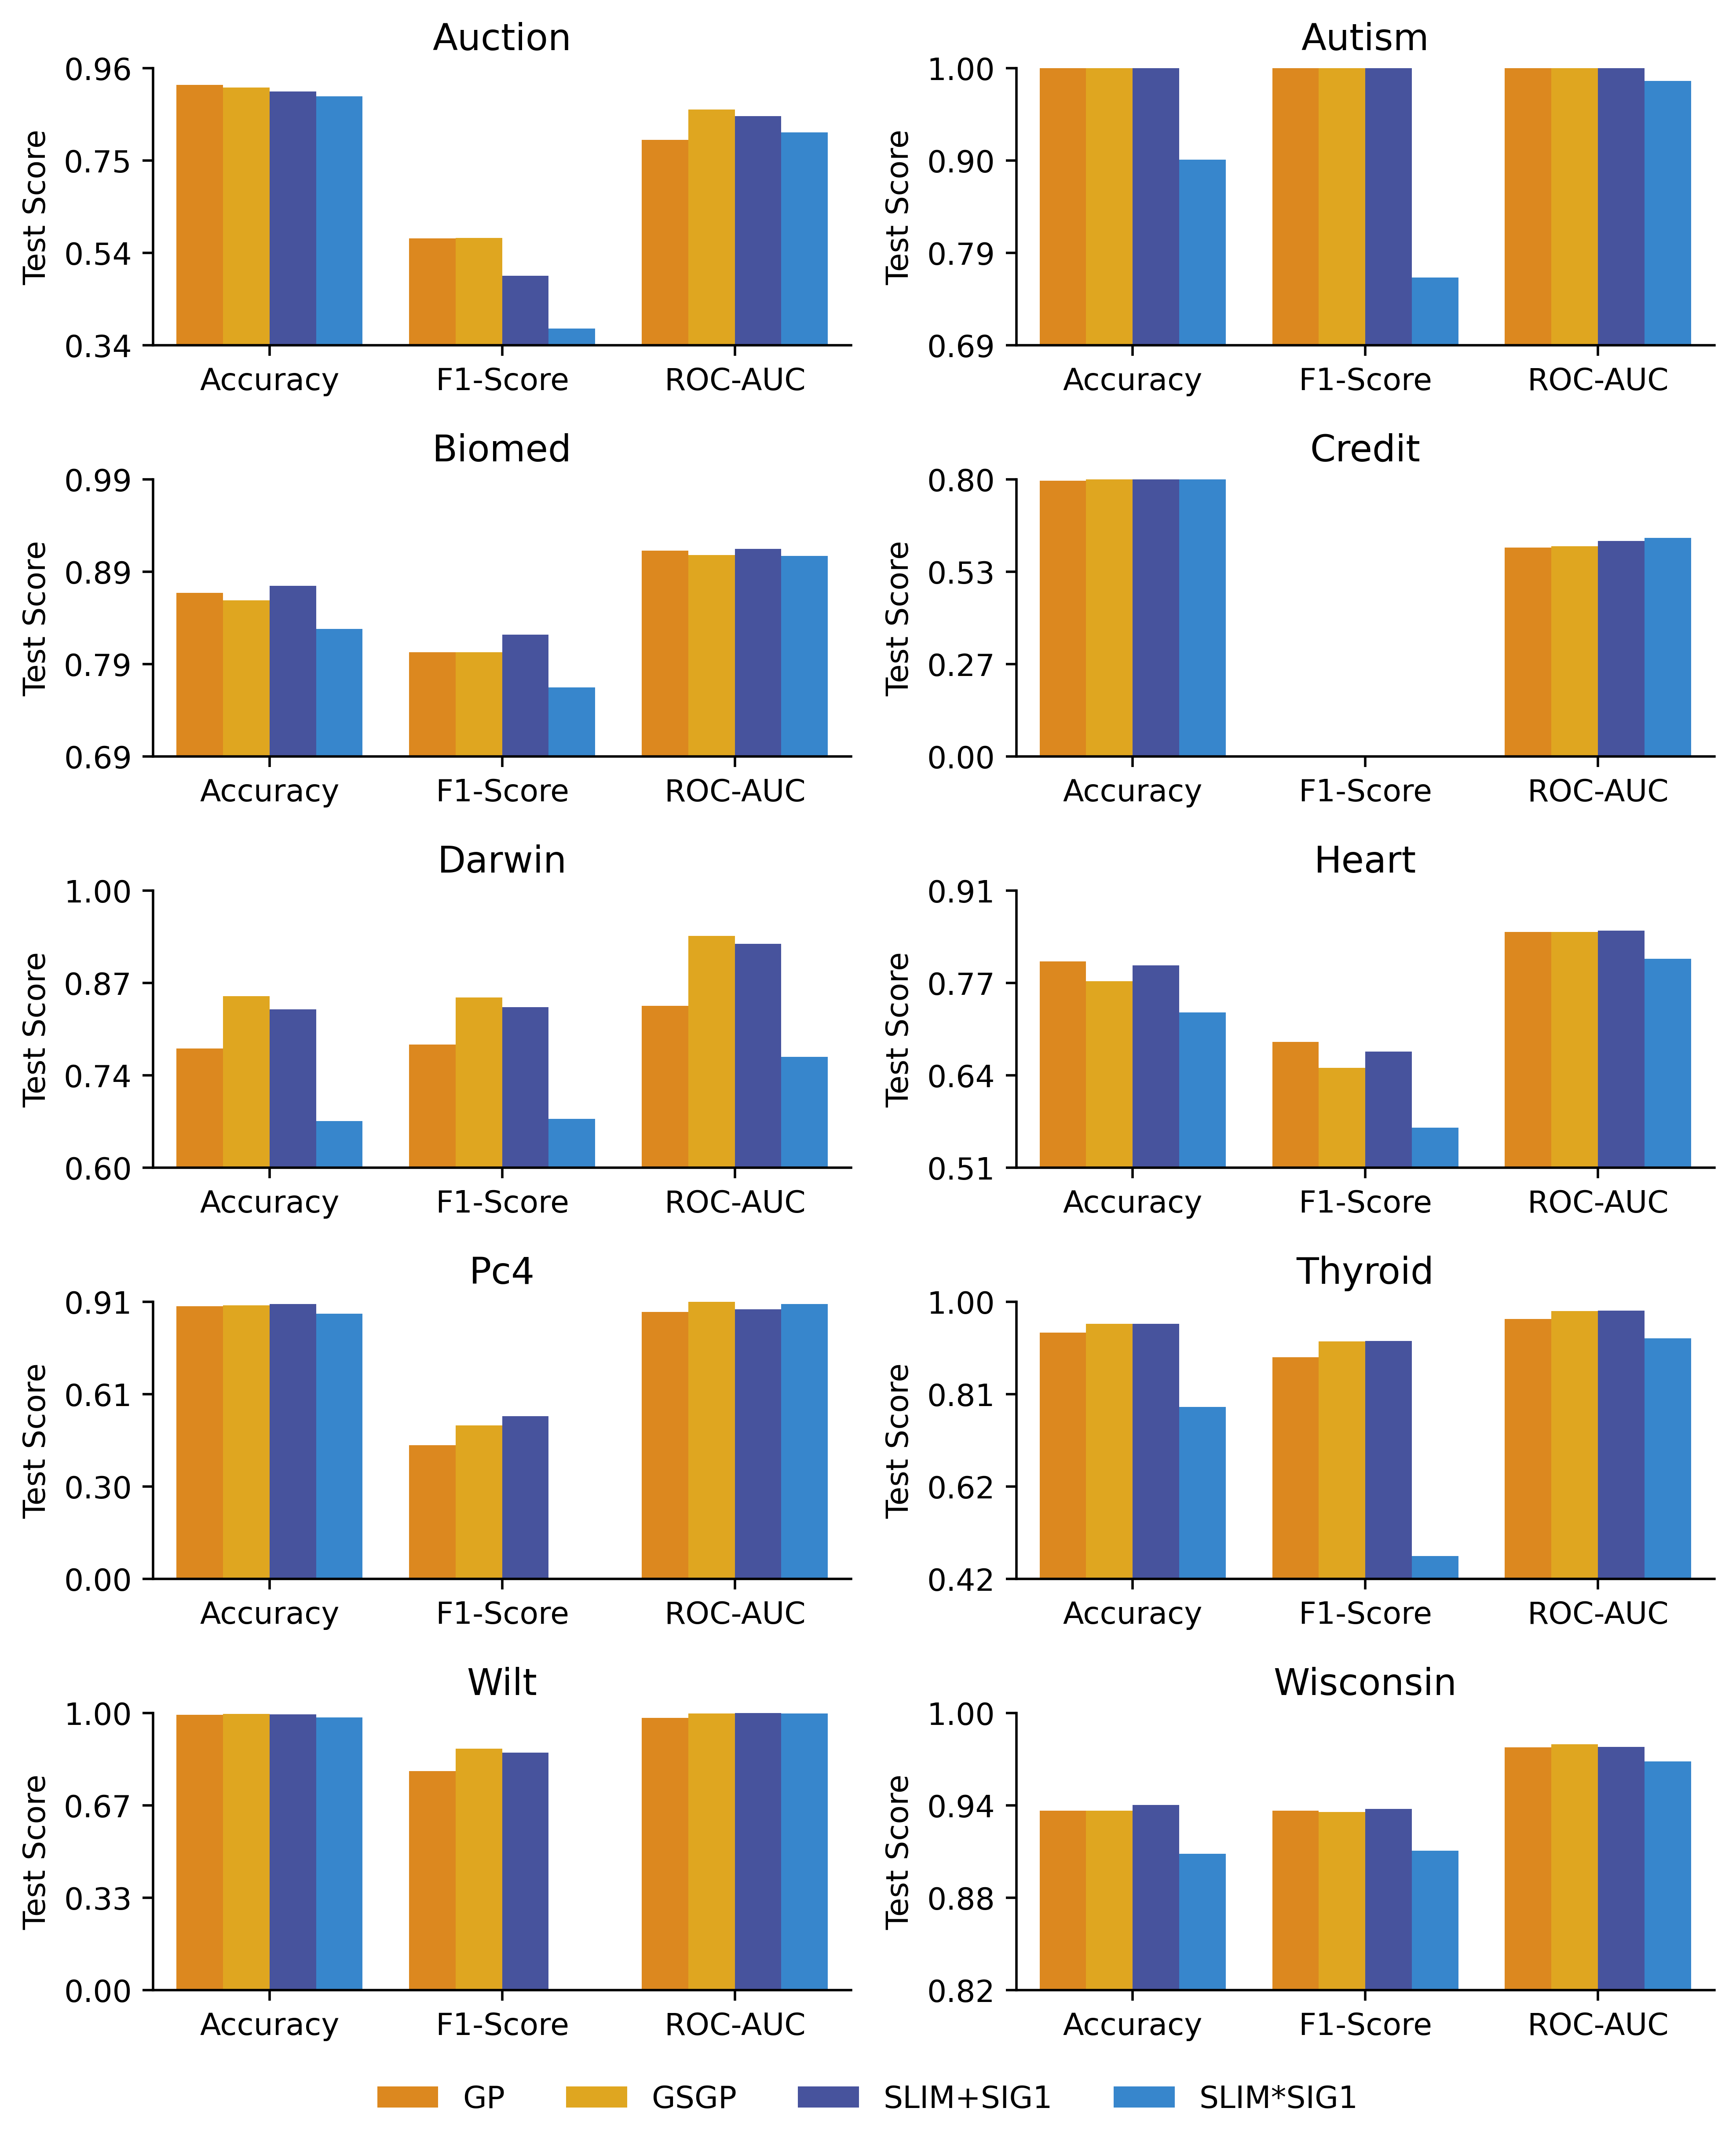
\includegraphics[width=\linewidth]{../Latex/Chapters/Figures/Results/RQ_Comparison_performance.png}
    \caption{Performance by Algorithm}
    \label{fig:RQ_Comparison_performance}
    \end{figure}
    





\end{document}
\endinput
%%
%% End of file `sample-acmsmall.tex'.
